\section{Signal Modeling}
\label{sec:signal_model}

% % TODO: add a reference to ad hoc studies in appendix in this section?

% \subsection{\texorpdfstring{\Zone}{Z1} Mass Constraint}  % TODO: Makes Z1 in subsection title NOT bold.
% % \subsection{\texorpdfstring{\boldmath{\Zone}}{Z1} Mass Constraint} % TODO: Although \boldmath makes \subsection bold, it also makes the TOC entry bold.

% \subsection{Per-Event Relative Mass Error Categorization}
% \subsection{VXBS Constraint}

% %=== Hualin's thesis ===%
% % \subsubsection{Computation of Per-Event Mass Uncertainties}
% % \subsubsection{Correction of Lepton Momentum Uncertainties}
% % \subsubsection{Model and Procedure to Derive Corrections}
% % \subsubsection{Validation of Corrections}
% %=== AN-19-248 ===%
% % \subsubsection{motivation}
% % \subsubsection{model and procedure to derive Corrections}
% % \subsubsection{validation of corrections (MC, data)}

% \subsection{Matrix Element-Based Kinematic Discriminant}

% \begin{table}[ht]
%     \begin{center}
%     \begin{tabular}{|c|cccc|c|}
%     \hline			
%     Expected uncertainty	&	4$\mu$	&	4e	&	2e2$\mu$	&2$\mu$2e	& Inclusive	\\
%     \hline			
%         1D	(No bkg) &	153	&	466	&	315	&	300	&	121	\\
%     \hline
%     \end{tabular}
%     \end{center}
%     \caption{
%         %=== Below is the description from AN-19-248. ==%
%         % Expected Higgs boson mass uncertainty measured with 1D model 
%         % for different final states. All mass values are given in \MeV.
%         % Statistical only results are considered at this stage of the analysis.
%         }
%     \label{table:model_result_fs_1D}
%     \end{table}




%=== FROM AN but modified. ===%
%\subsection{Signal correction}
%\label{sec:SignalCorrection}
%The dominant POWHEG ggF process is reweighted to the NNLOPS one, using bins of generated Higgs 
%$p_{T}$ and number of generated jets. More details in \cite{HIG_19_001}.
% TODO:REWORD
\subsection{Signal Normalization}
\label{sec:SignalNormalization}
The normalization of the Higgs boson signal is obtained, from simulation, 
looking at the expected signal yields in the range [105, 140] GeV, 
for five simulated mass points (120, 124, 125, 126 and 130 GeV).
A second order polynomial function is used to extract the dependence of the normalization from $m_{H}$.
Fits are performed separately for each production mode, for each decay channel and for each year. 
Examples of the fits can be observed in Fig.~\ref{fig:signal_normalization}
\begin{multiFigure}
    \centering
    \addFigure{0.48}{figures/higgsmassmeas/signal_norm/NoZ1/2016pre_ggH_yield.pdf}
    \addFigure{0.48}{figures/higgsmassmeas/signal_norm/NoZ1/2016post_ggH_yield.pdf}
    \addFigure{0.48}{figures/higgsmassmeas/signal_norm/NoZ1/2017_ggH_yield.pdf}
    \addFigure{0.48}{figures/higgsmassmeas/signal_norm/NoZ1/2018_ggH_yield.pdf}
    \captionof{figure}
        [TODO]
        {Normalization fit for ggH, in different decay channels, as a function of mass, for 2016 on top (pre-VFP on the left, post-VFP on the right), 2017 on bottom left, 2018 on the bottom right.}
    \label{fig:signal_normalization}
\end{multiFigure}
%%%%%%% 
%%%%%%% 
% plots about normalisation will be shown only for 1D_VXBS_Z1 configuration
%%%%%%% 
%%%%%%% 
%
%\begin{figure}[!htbp]
%	\begin{center}
%   		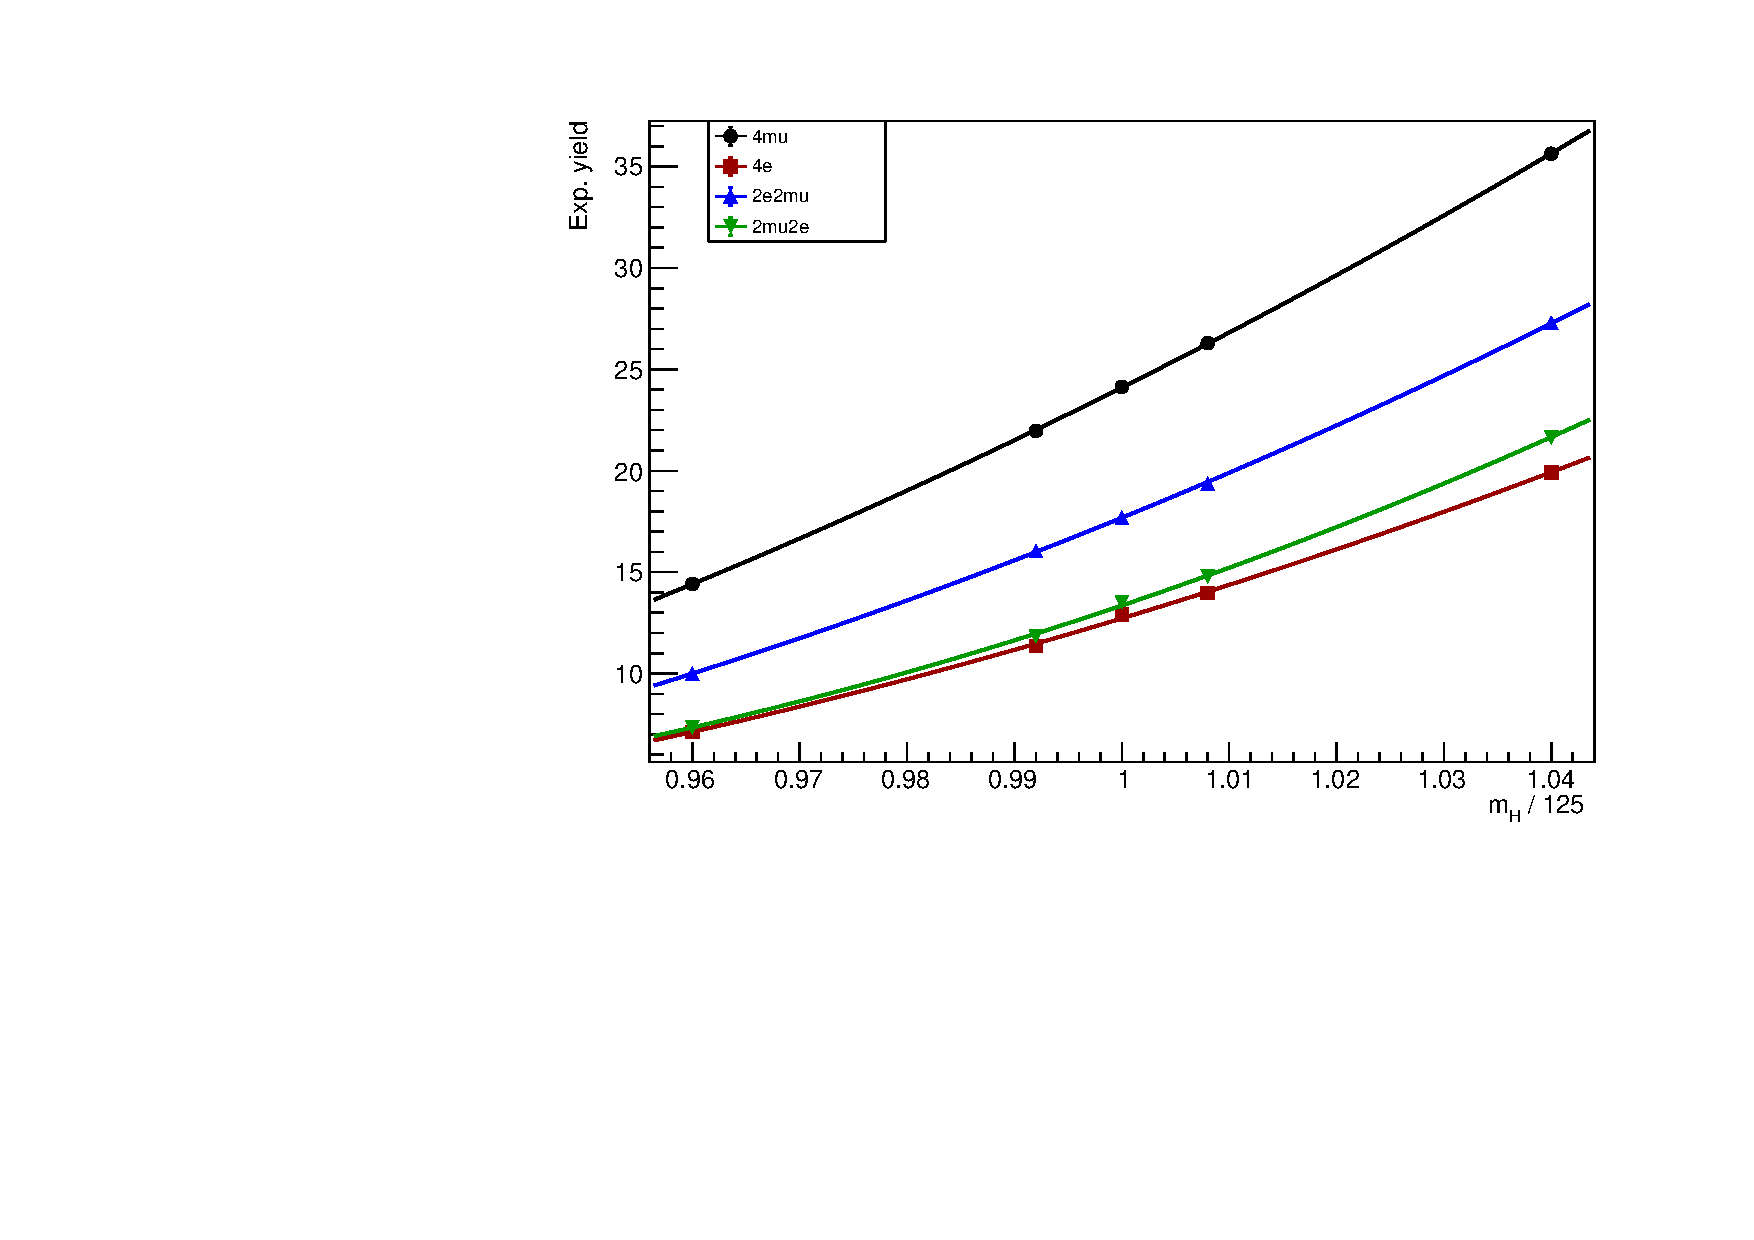
\includegraphics[width=0.3\textwidth]{Figures/SignalModelling/Signal_Normalisation/NoZ1/2017_ggH_yield.pdf}
%		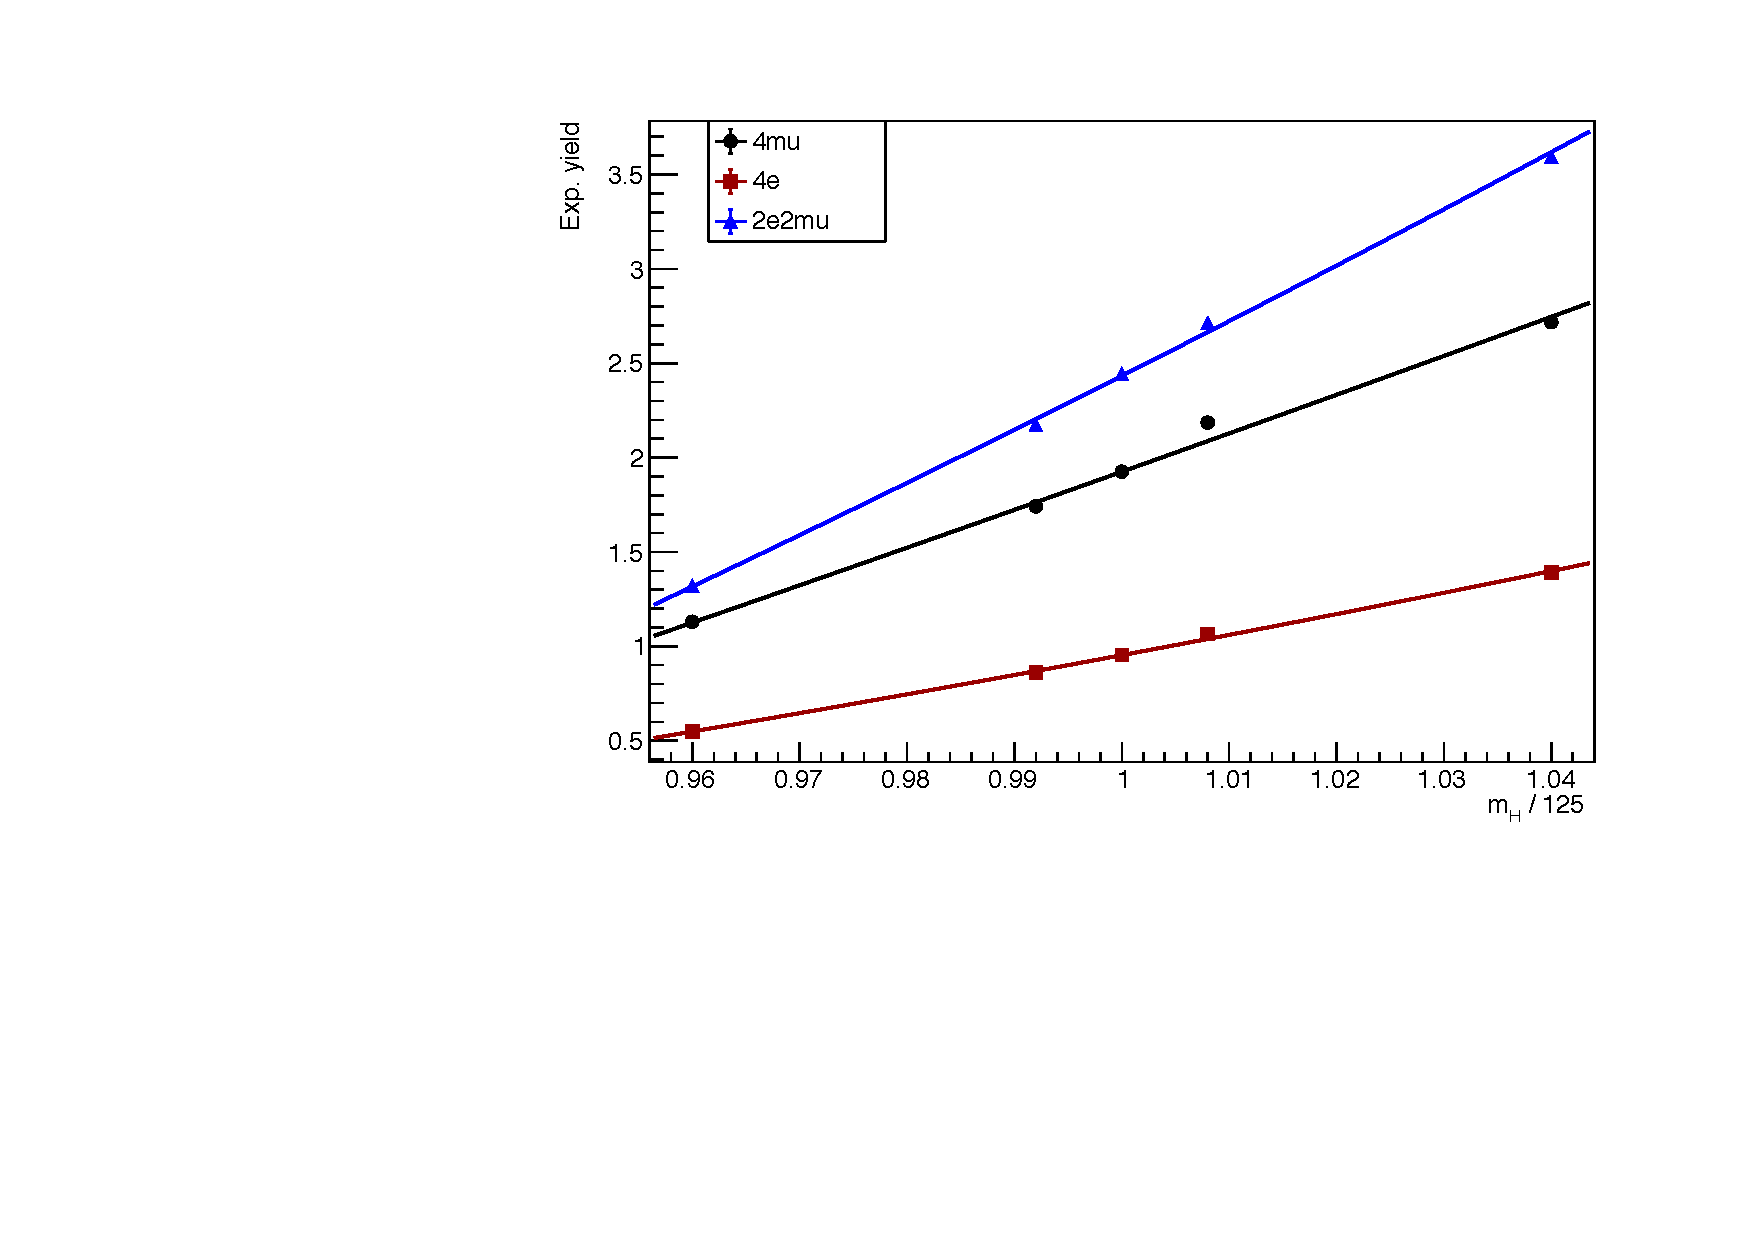
\includegraphics[width=0.3\textwidth]{Figures/SignalModelling/Signal_Normalisation/NoZ1/2017_VBF_yield.pdf} 
%		\includegraphics[width=0.3\textwidth]{Figures/SignalModelling/Signal_Normalisation/NoZ1/2017_ZH_yield.pdf}
%		\caption{Normalization fit in 2017, for different decay channels, as a function
%		of mass, for ggH on the left, VBF in the middle, ZH on the right.}
%	\label{signal_normalization_2017}
%	\end{center}
%\end{figure}
%
%\begin{figure}[!htbp]
%	\begin{center}
%   		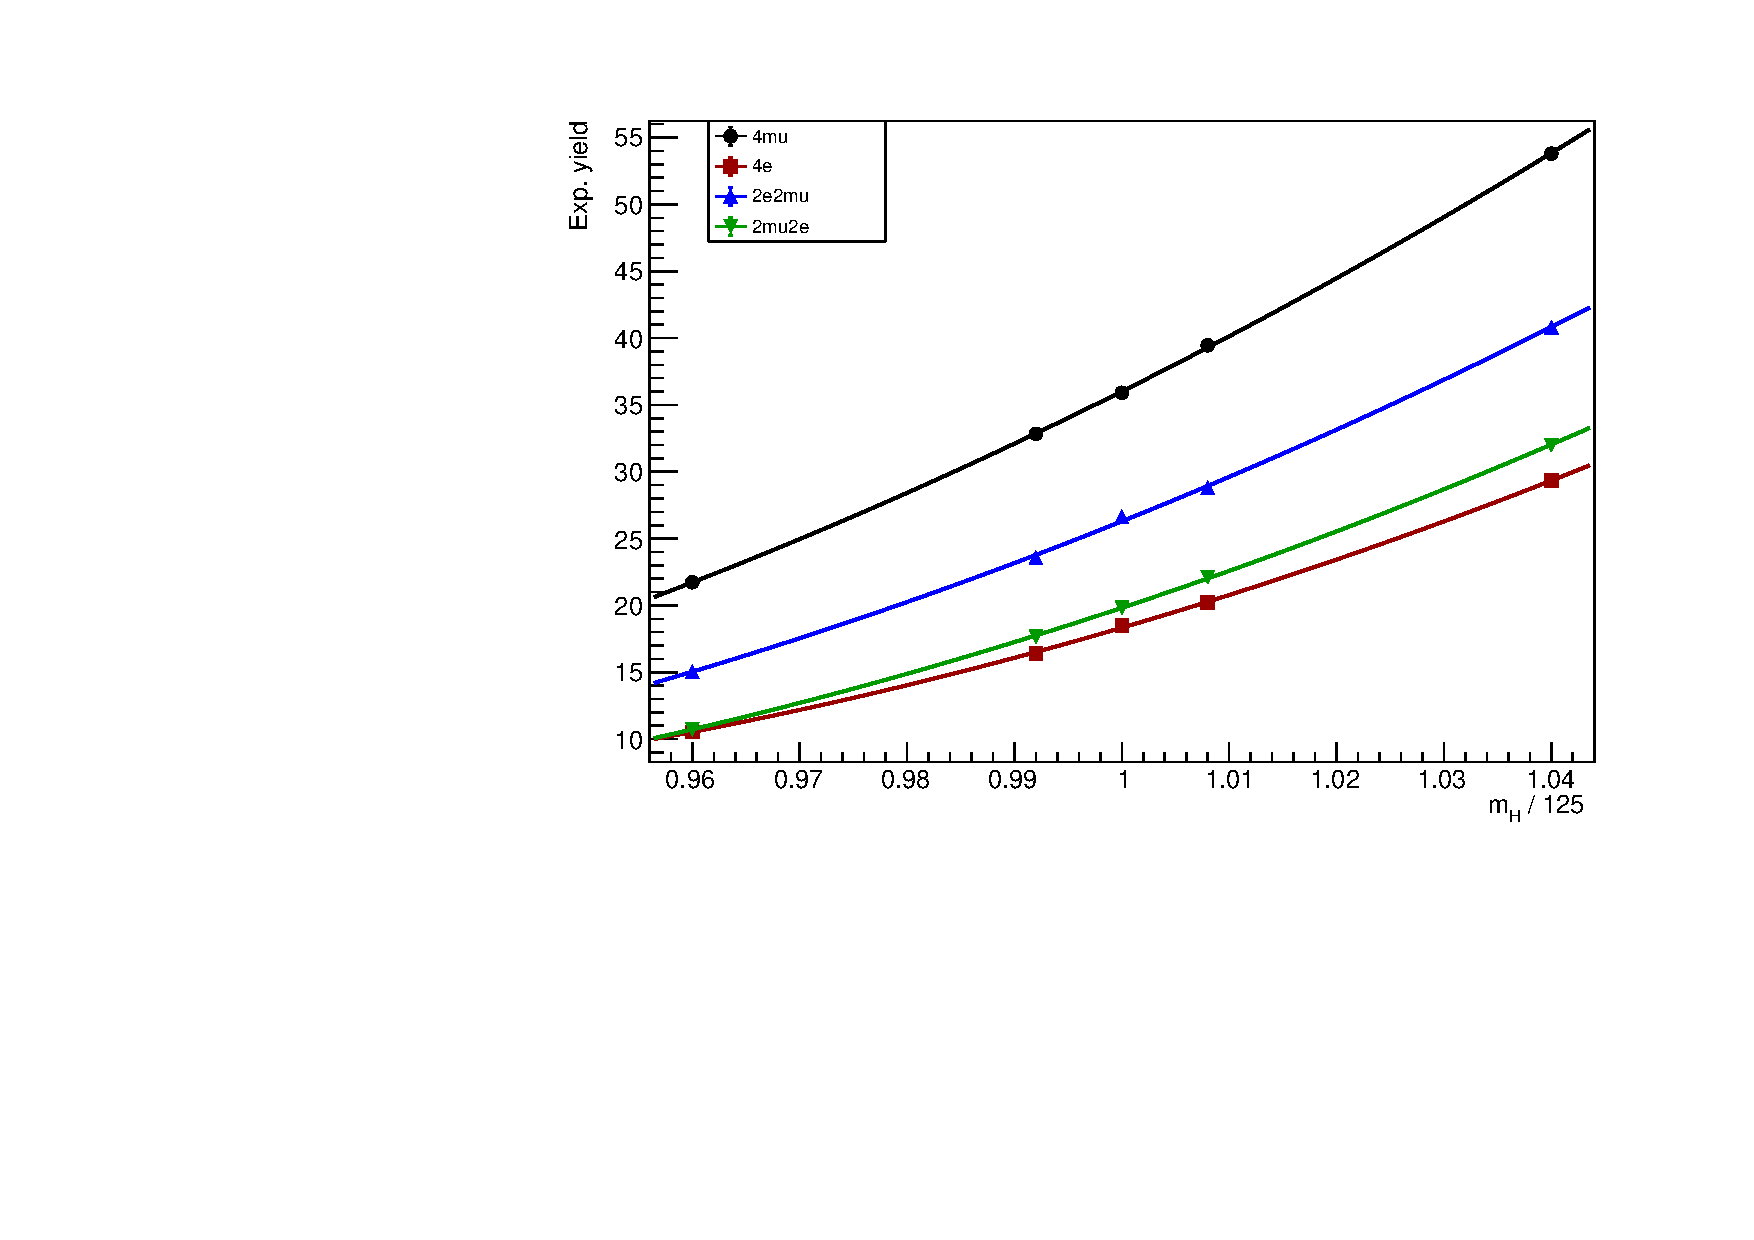
\includegraphics[width=0.3\textwidth]{Figures/SignalModelling/Signal_Normalisation/NoZ1/2018_ggH_yield.pdf}
%		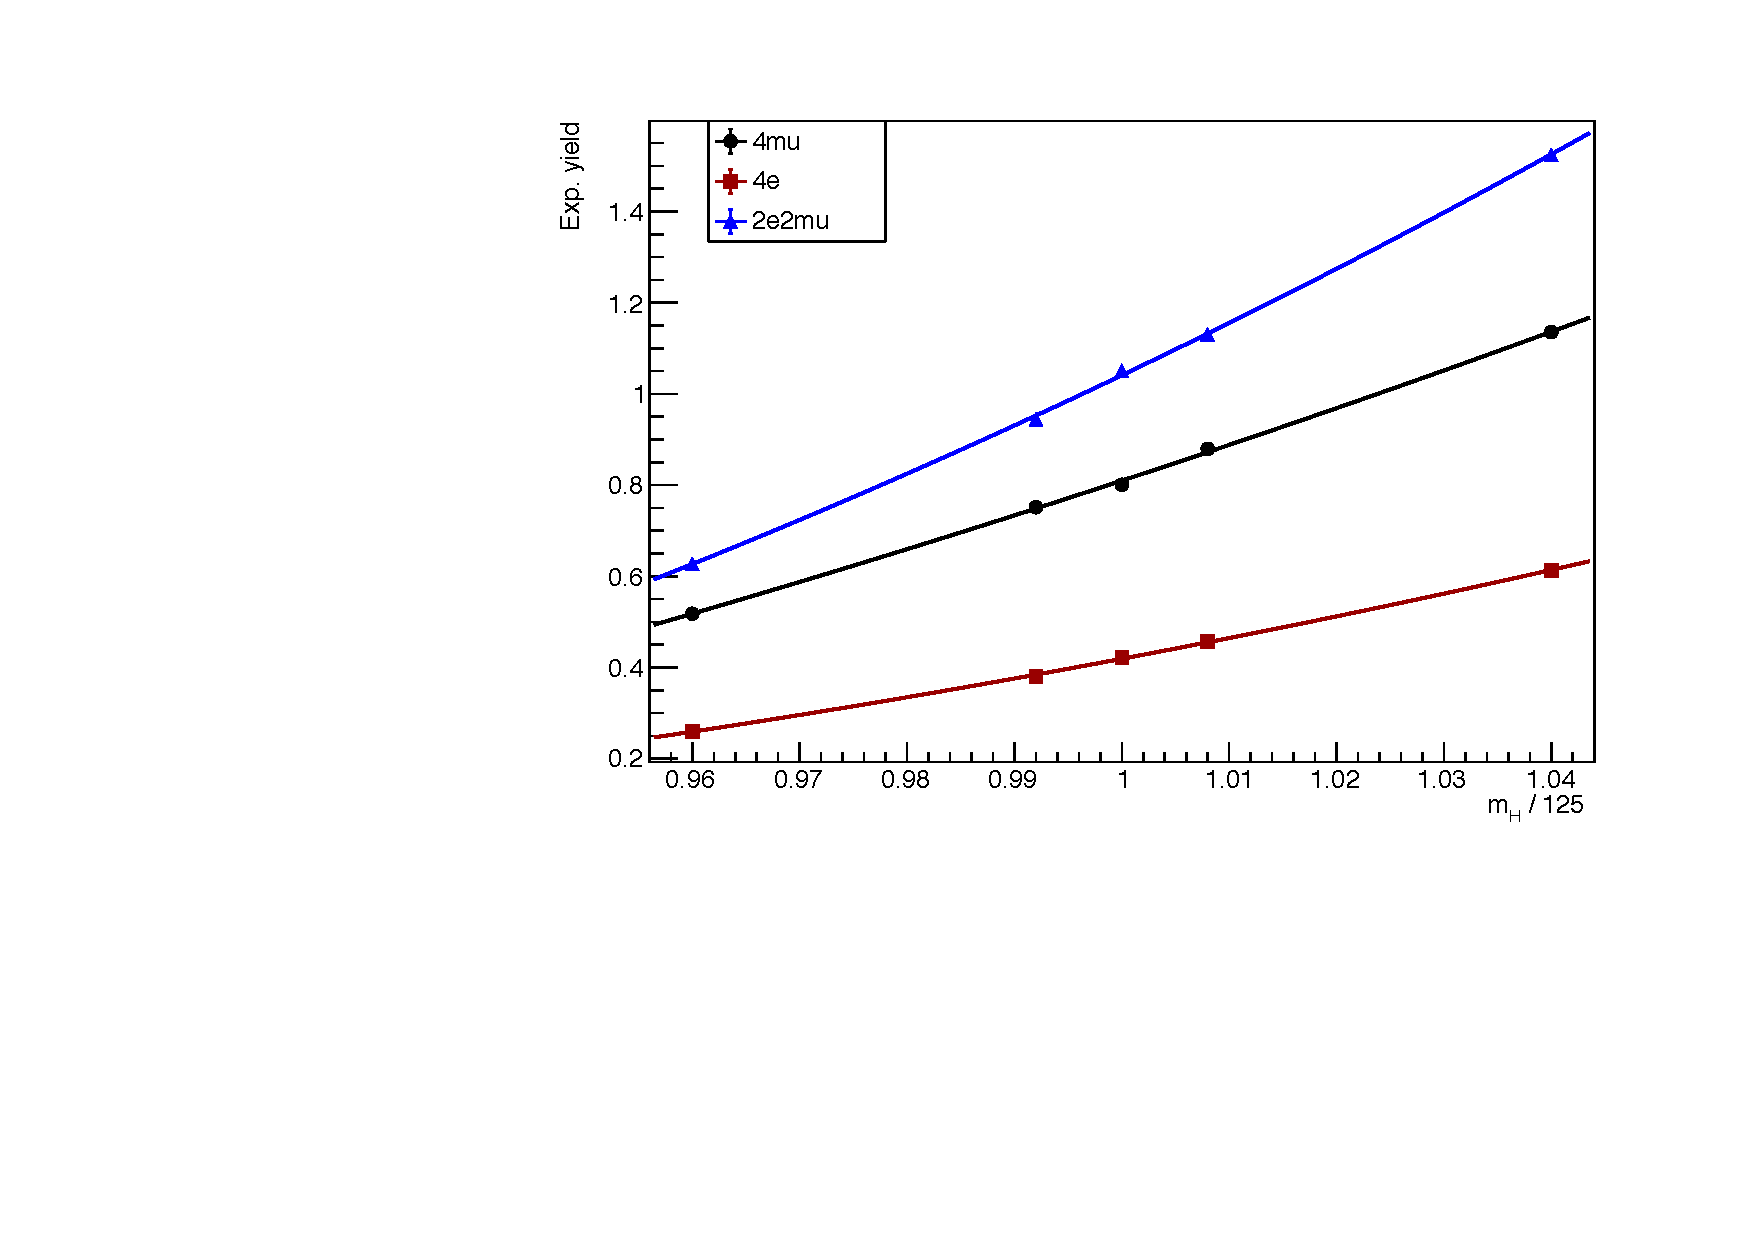
\includegraphics[width=0.3\textwidth]{Figures/SignalModelling/Signal_Normalisation/NoZ1/2018_WH_yield.pdf} 
%		\includegraphics[width=0.3\textwidth]{Figures/SignalModelling/Signal_Normalisation/NoZ1/2018_ttH_yield.pdf}
%		\caption{Normalization fit in 2018, for different decay channels, as a function
%		of mass, for ggH on the left, WH in the middle, ttH on the right.}
%	\label{signal_normalization_2018}
%	\end{center}
%\end{figure}

\subsection{Parameterizing the Signal Mass Line Shape}
\label{sec:SignalParametrization}
The signal lineshape is obtained from the fit of the Higgs boson mass distribution, 
in the range [105, 140] GeV, using a double-sided Crystal Ball (DSCB) function, which
has 6 parameters.
%This function has six independent parameters, 
%with a Gaussian core ($\sigma_{m}$) that describes the four-lepton mass resolution function and 
%the systematic mass shift ($\Delta m_{H}$) of the peak, and the left- and right-hand tail 
%originating from leptons emitting brem in the tracker material, present for both electrons and muons, 
%and from the non-Gaussian mis-measurements specific to interactions of electrons with the detector material 
%(each side of the distribution is described by two parameters, n and $\alpha$).\\
 Fit parameters are derived as a function of mass, using a first order polynomial:
%\textbf{Compare first vs second order formula: current results with second one}
 \[
 param^{i}_{DSCB} = a^i + b^{i}~(m_{H} - 125)% + c~(m_{H} - 125)^{2}
 \]
 
 First, from the fit of the only 125 GeV sample, the ``a'' term for each parameter is extracted
 (``b'' term in this case is not taken into account). Then, a second fit is performed: this time,
 ``a'' is fixed to the value found before, while ``b'' is kept free to float
     when fitting all five different mass points (120, 124, 125, 126, 130\GeV) simultaneously. \\
 The fit is performed separately, for each production mode, for each decay channel, in each year. 
 To take into account the non-resonant contribution in the case of VH and ttH production modes, the 
     DSCB is convoluted with a Landau function that describes the possibility for a 
     lepton from the Higgs boson decay to be lost or not selected.\\
%%%%%%% 
%%%%%%% 
% plots about normalisation will be shown only for 1D_VXBS_Z1 configuration
%%%%%%% 
%%%%%%% 
%Examples of the fit procedures are shown in \figurename~\ref{signal_lineshape_2016}, \ref{signal_lineshape_2017}, 
%\ref{signal_lineshape_2018} for 125 GeV sample, and in  \figurename~\ref{signal_lineshape_2016_full_1}, 
%\ref{signal_lineshape_2016_full_2}, \ref{signal_lineshape_2017_full_1}, 
%\ref{signal_lineshape_2017_full_2}, \ref{signal_lineshape_2018_full_1} and  
%\ref{signal_lineshape_2018_full_2}, for the simultaneous fits.
%\begin{figure}[!htbp]
%	\begin{center}
%   		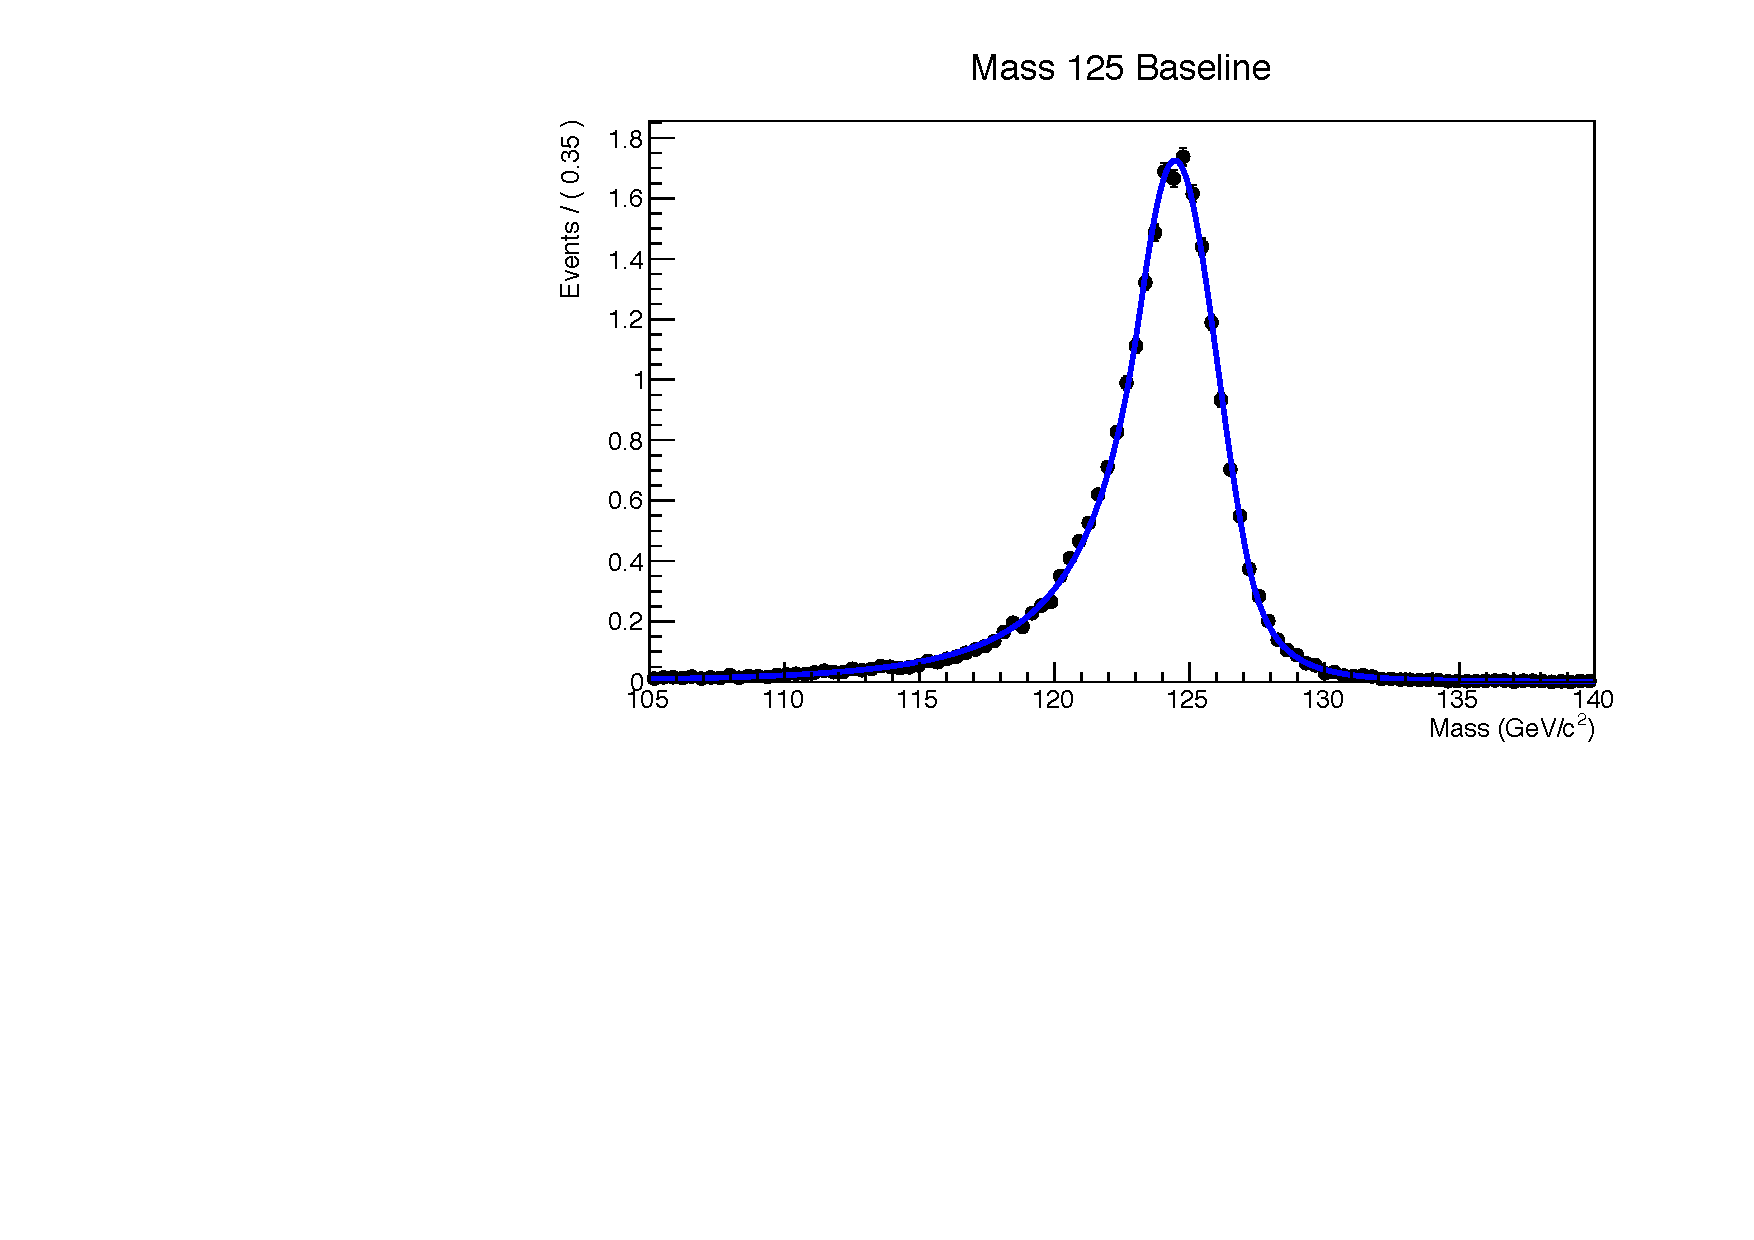
\includegraphics[width=0.3\textwidth]{Figures/SignalModelling/Signal_Parametrization/2016/ggH_2e2mu_2016_125.pdf}
%		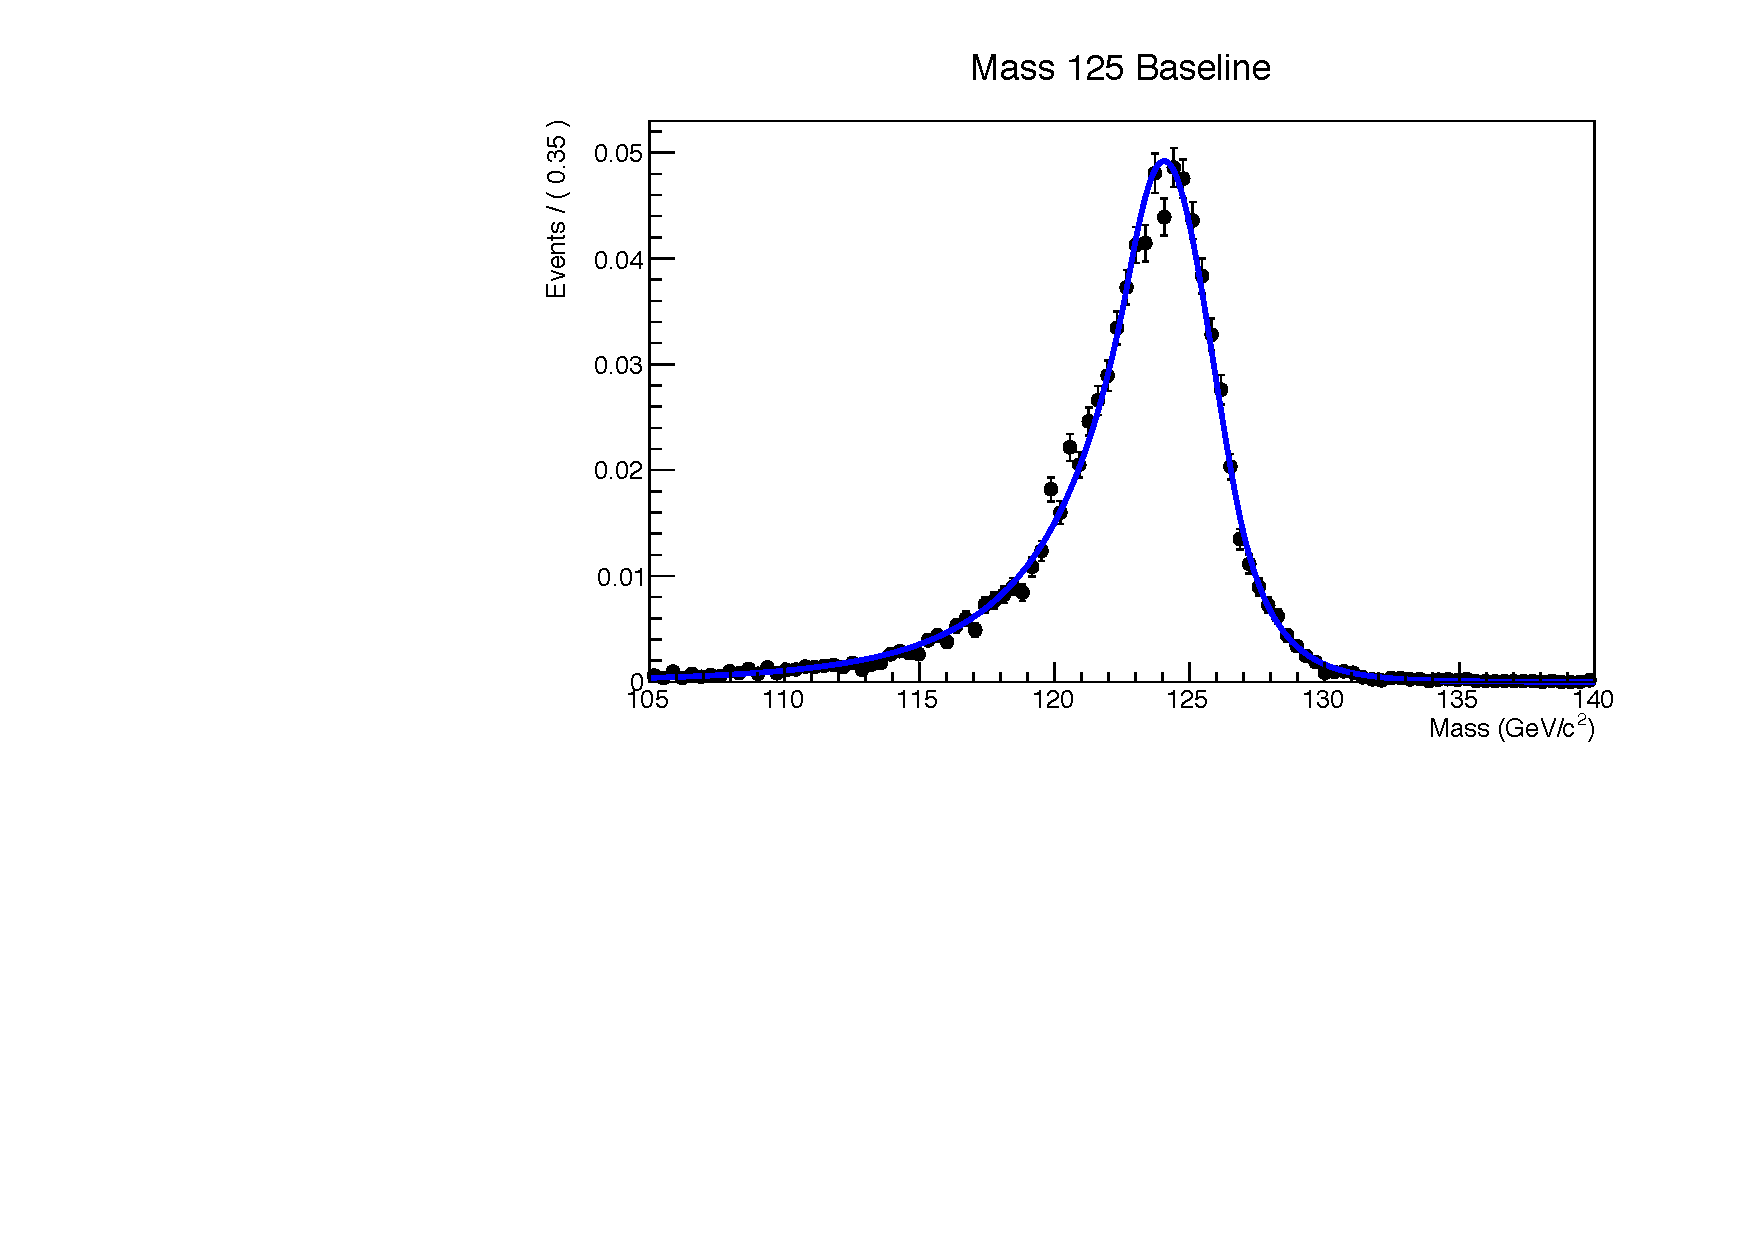
\includegraphics[width=0.3\textwidth]{Figures/SignalModelling/Signal_Parametrization/2016/VBF_4e_2016_125.pdf} 
%%		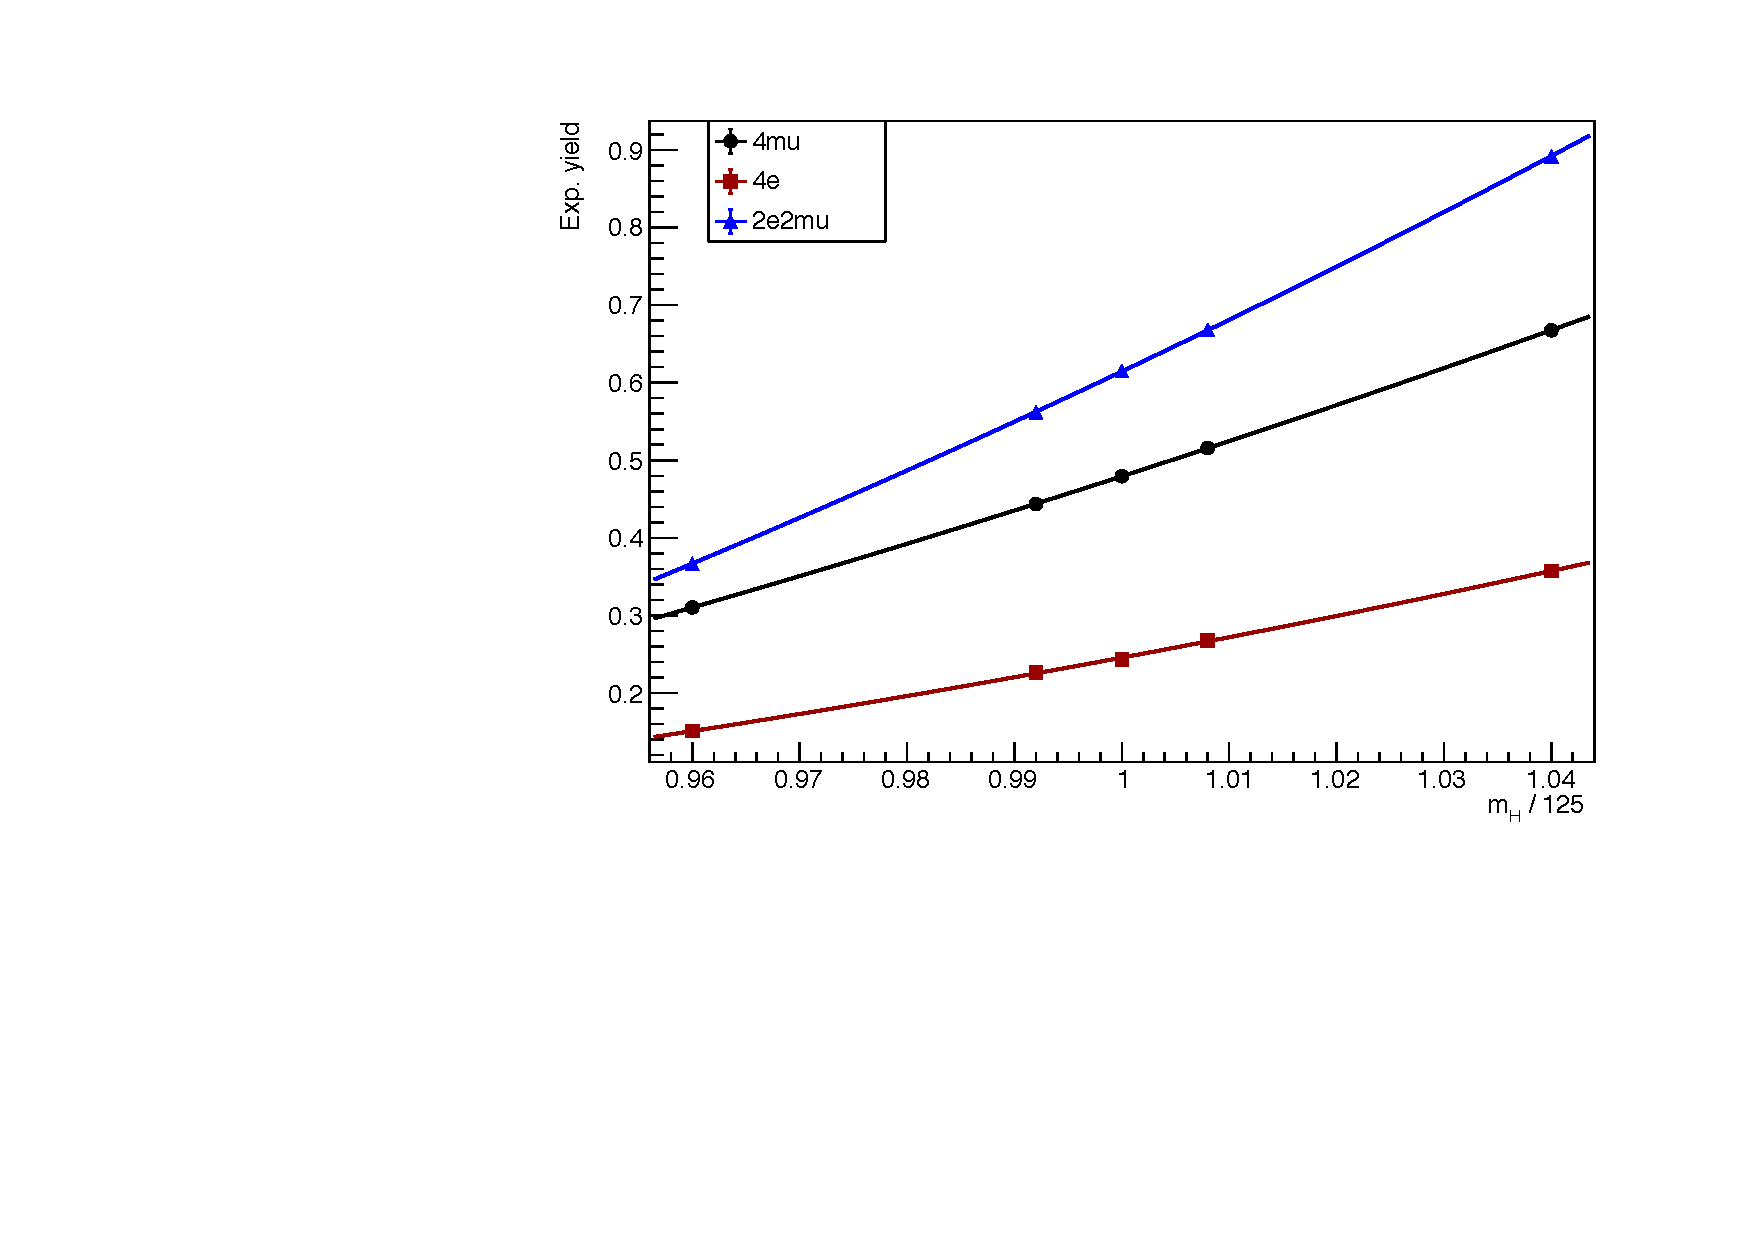
\includegraphics[width=0.3\textwidth]{Figures/SignalModelling/Signal_Parametrization/2016/2016_WH_yield.pdf}
%		\caption{125 GeV fit in 2016: 2e2$\mu$ ggF on the left, 
%		4e VBF on the right.}
%	\label{signal_lineshape_2016}
%	\end{center}
%\end{figure}
%\begin{figure}[!htbp]
%	\begin{center}
%   		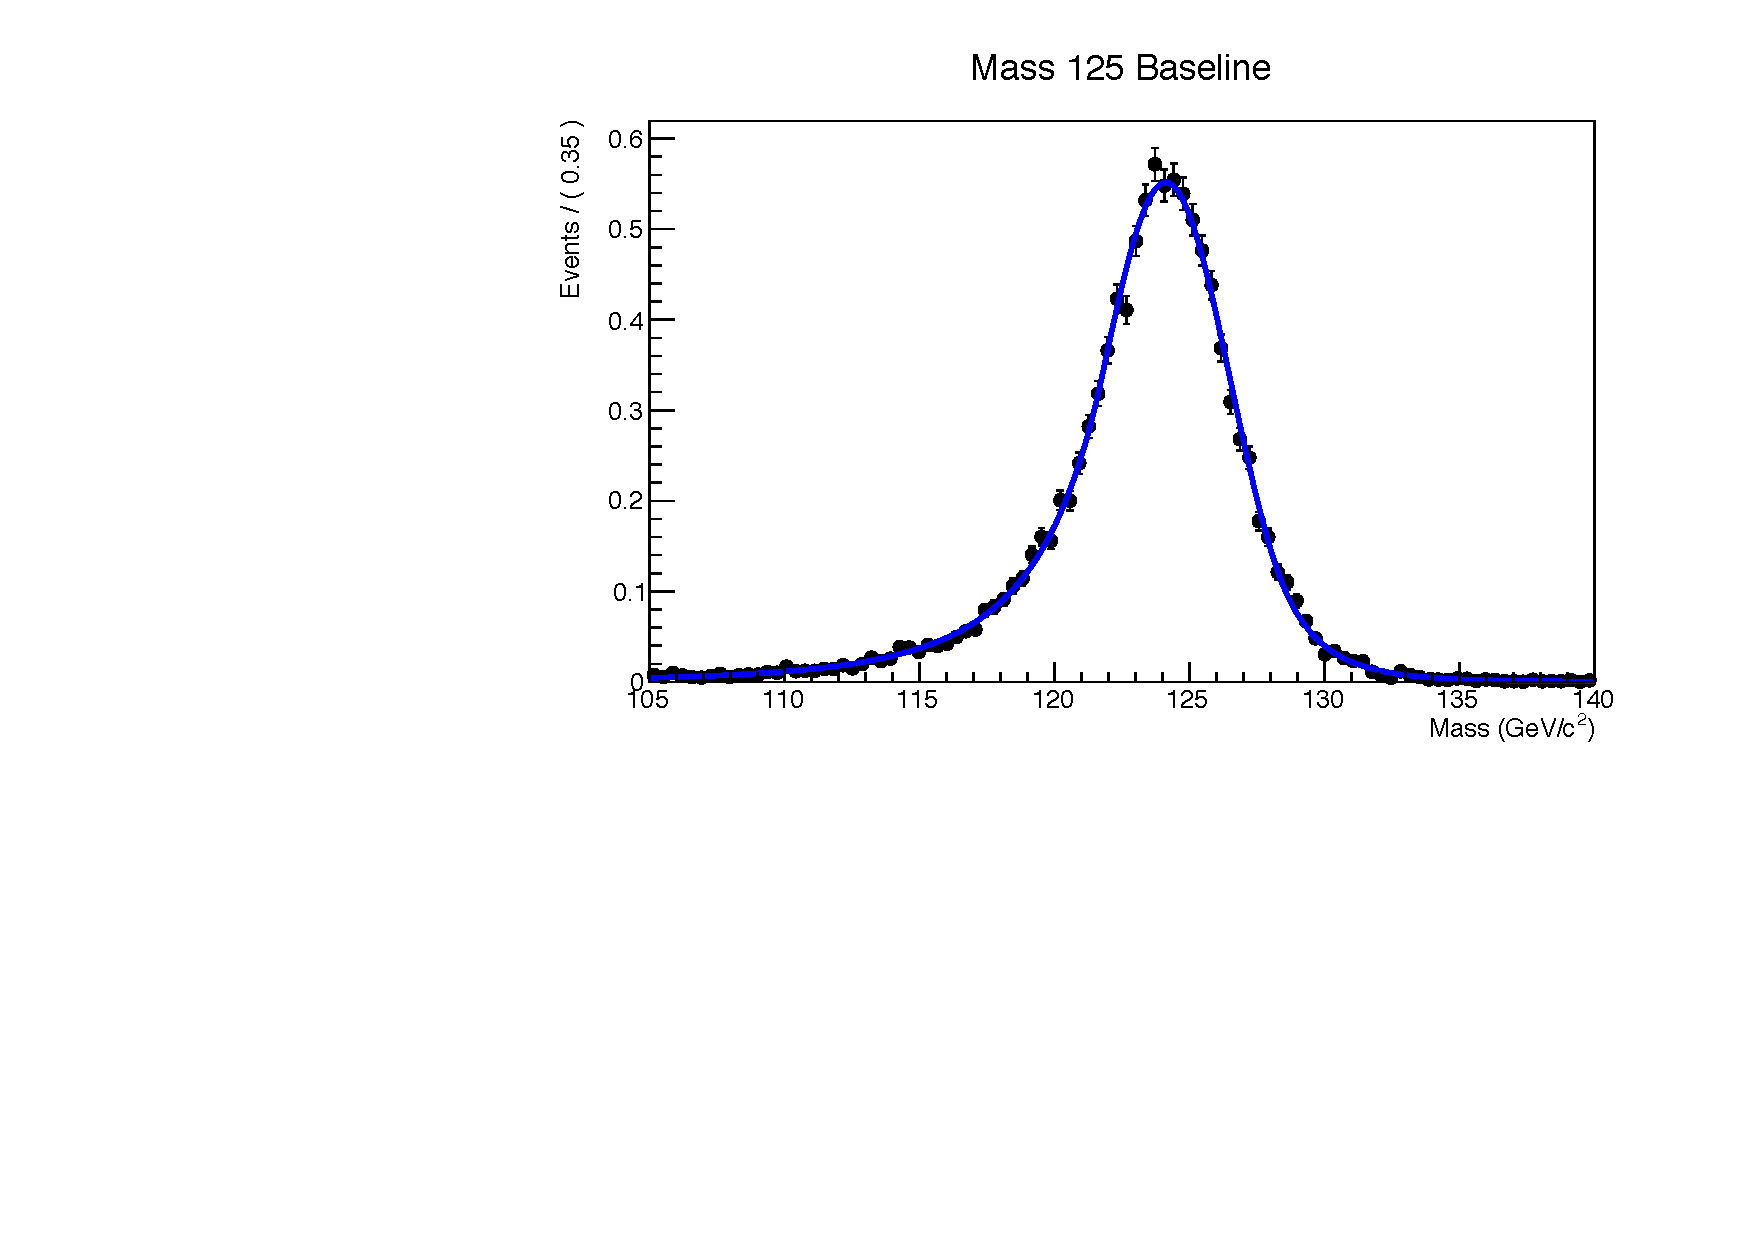
\includegraphics[width=0.3\textwidth]{Figures/SignalModelling/Signal_Parametrization/2017/ggH_4e_2017_125.pdf}
%		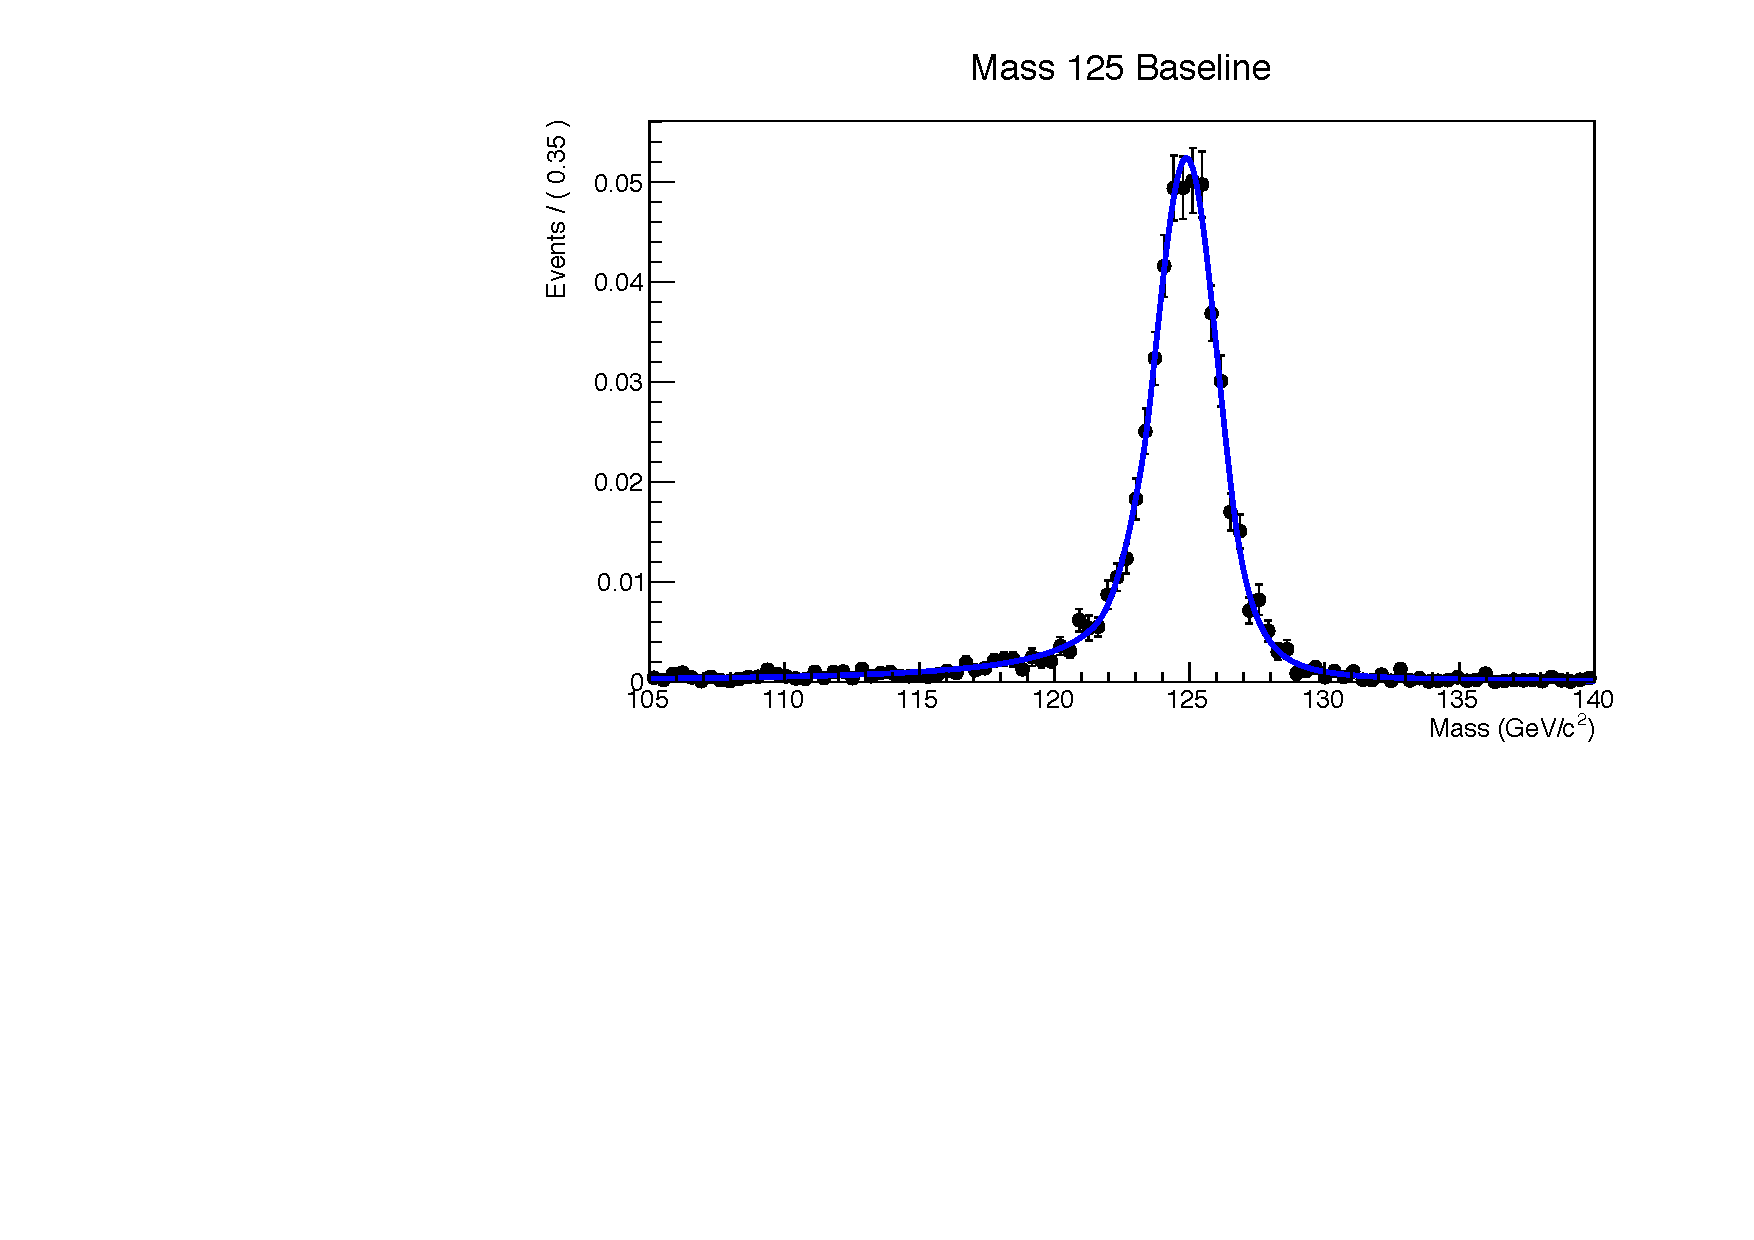
\includegraphics[width=0.3\textwidth]{Figures/SignalModelling/Signal_Parametrization/2017/WH_4mu_2017_125.pdf} 
%%		\includegraphics[width=0.3\textwidth]{Figures/SignalModelling/Signal_Parametrization/2017/2017_ZH_yield.pdf}
%		\caption{125 GeV fit in 2017: 4e ggF on the left, 
%		4$\mu$ WH on the right.}
%	\label{signal_lineshape_2017}
%	\end{center}
%\end{figure}
%\begin{figure}[!htbp]
%	\begin{center}
%   		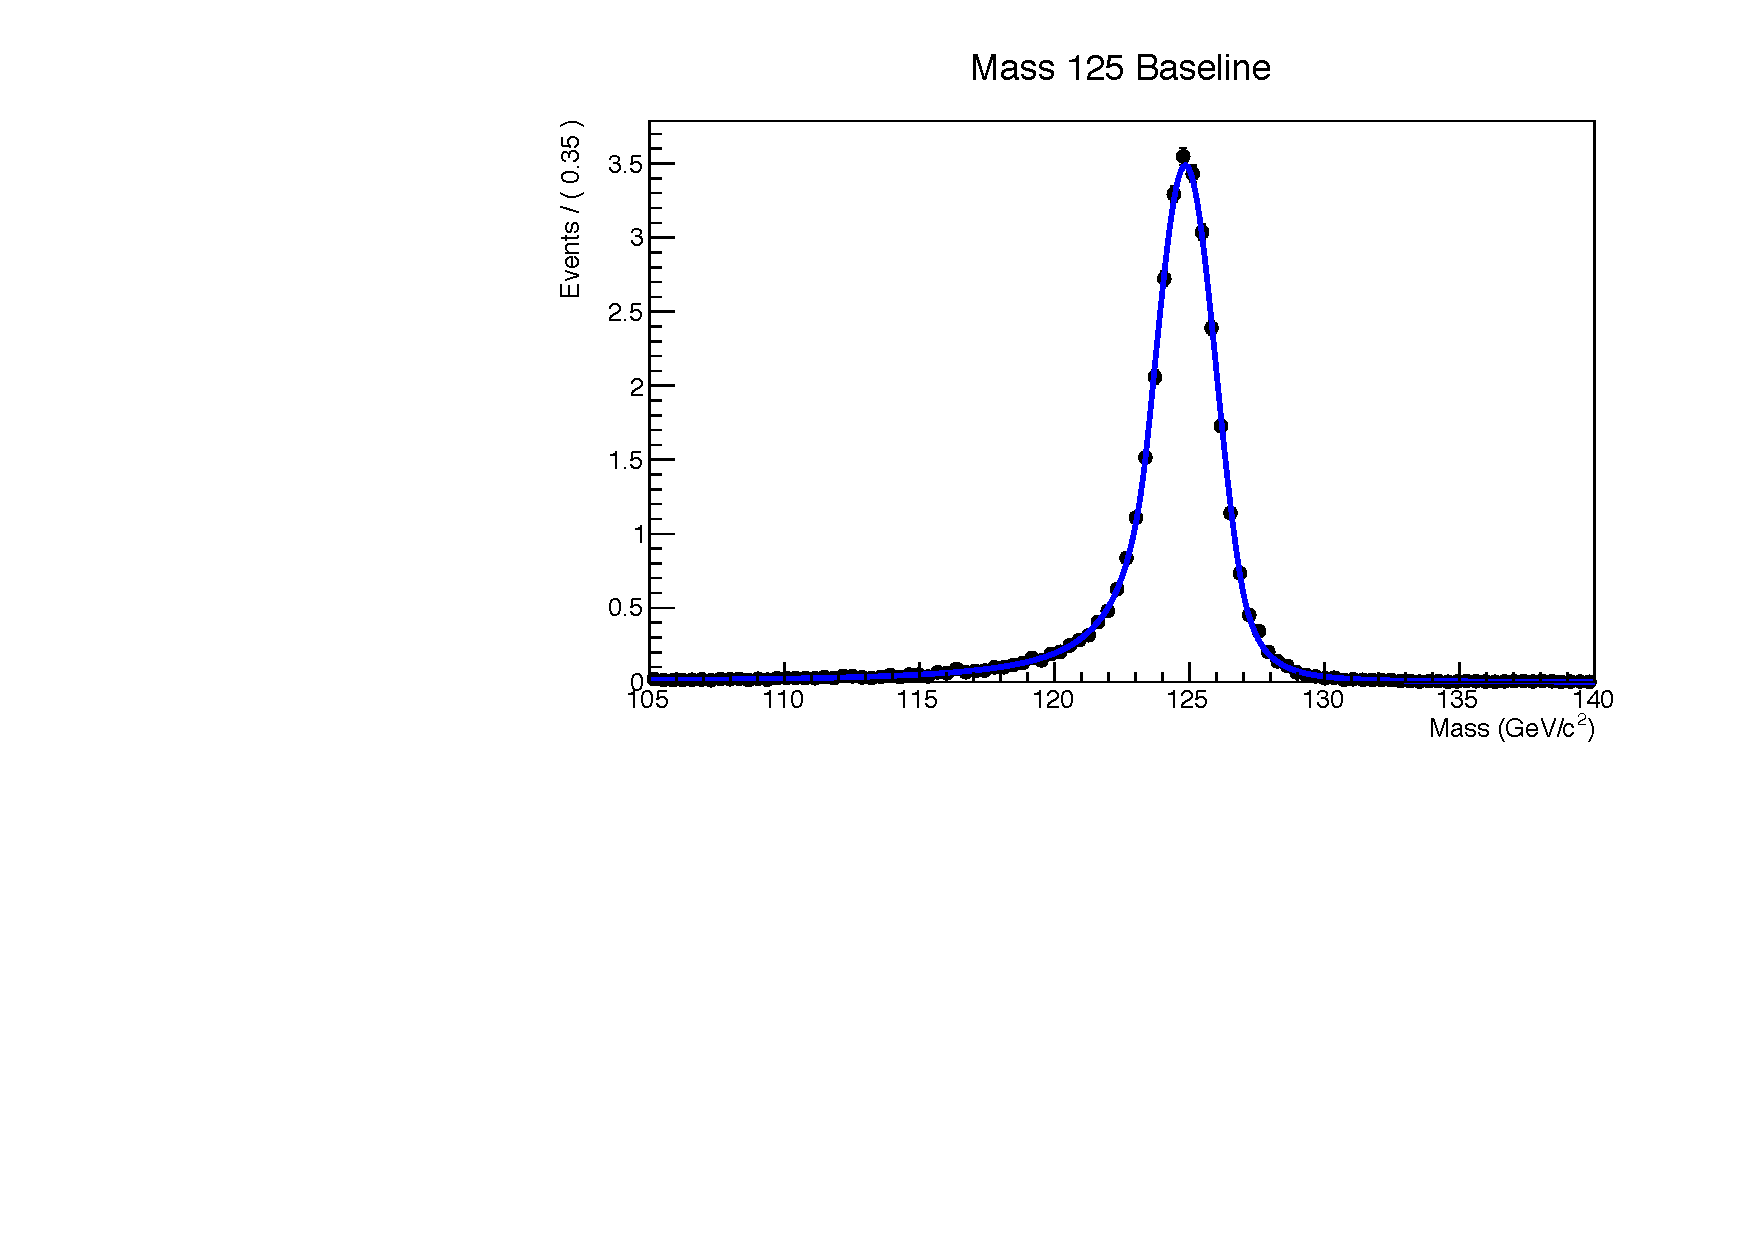
\includegraphics[width=0.3\textwidth]{Figures/SignalModelling/Signal_Parametrization/2018/ggH_4mu_2018_125.pdf}
%		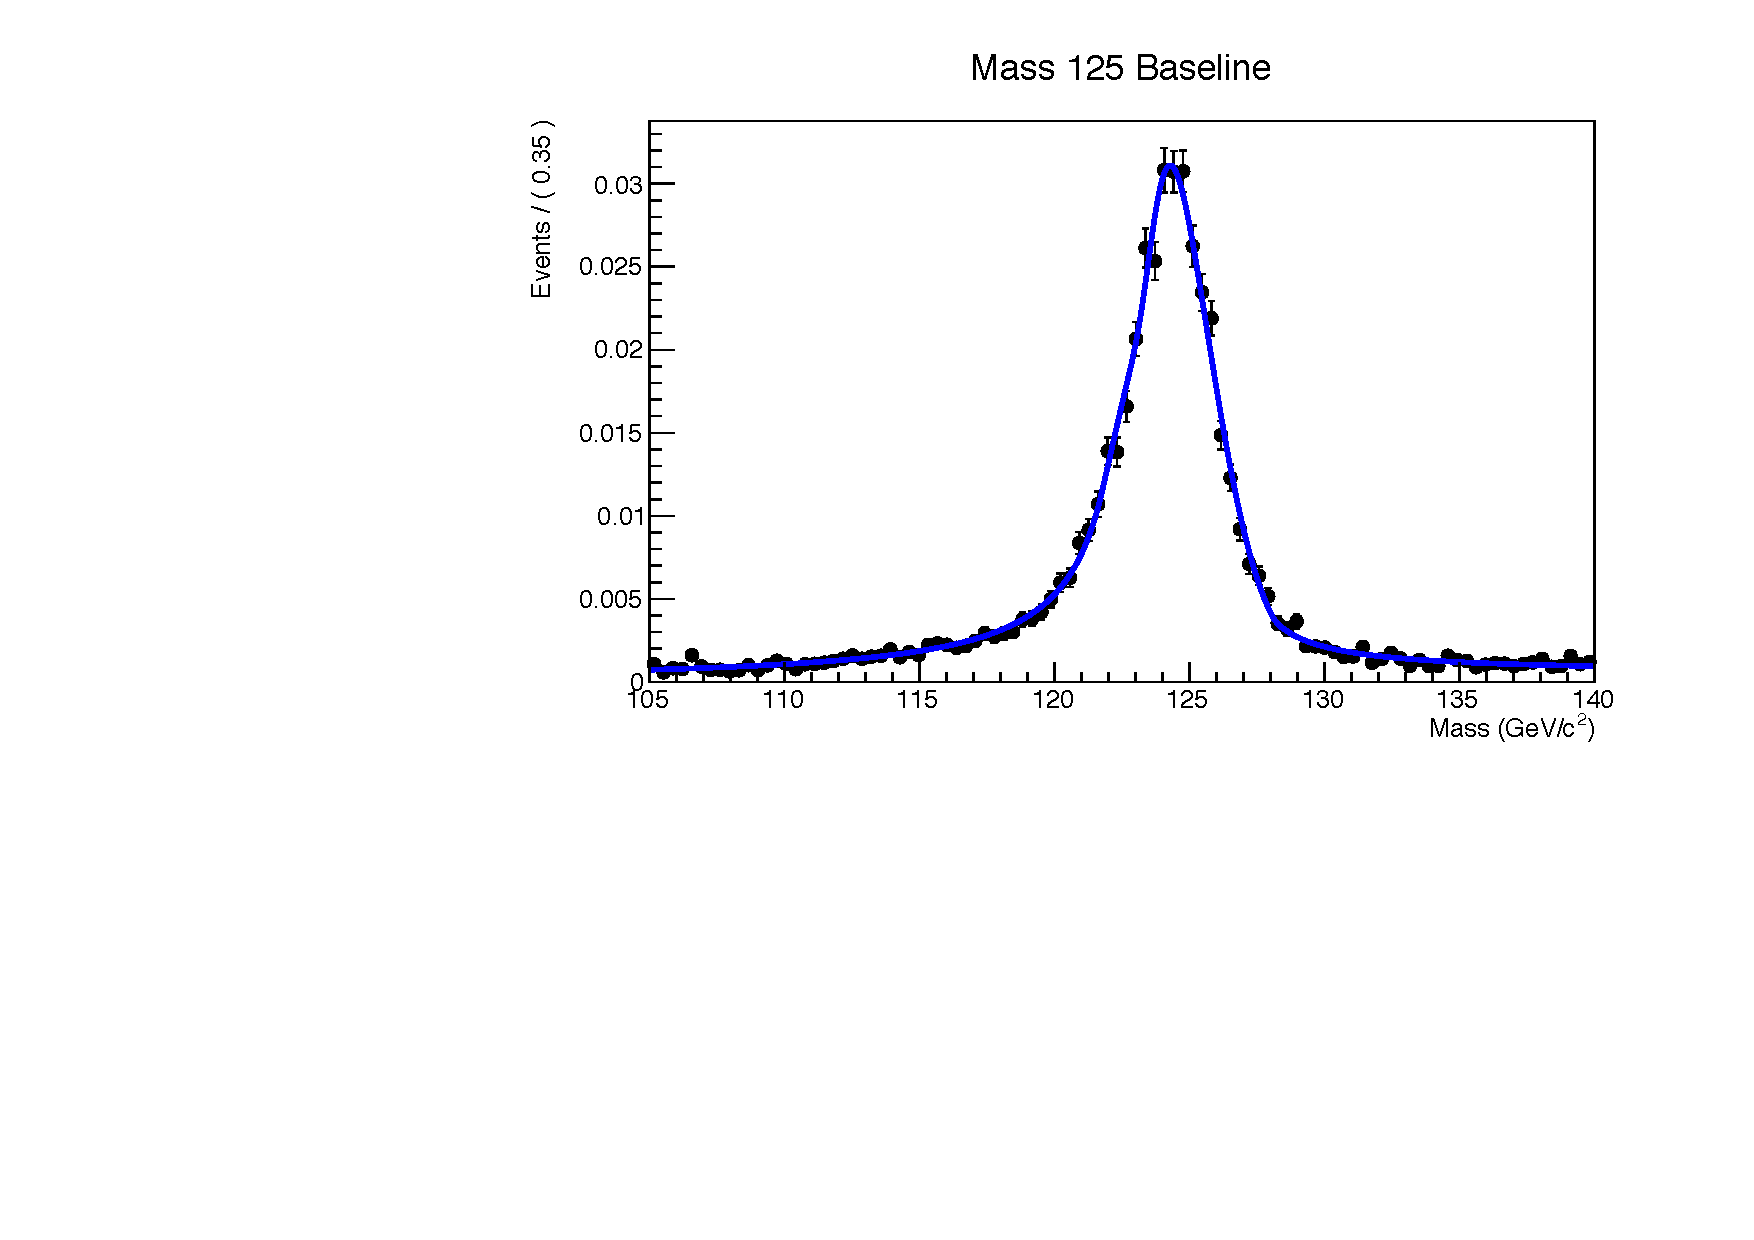
\includegraphics[width=0.3\textwidth]{Figures/SignalModelling/Signal_Parametrization/2018/ttH_2e2mu_2018_125.pdf} 
%%		\includegraphics[width=0.3\textwidth]{Figures/SignalModelling/Signal_Parametrization/2017/2018_ttH_yield.pdf}
%		\caption{125 GeV fit in 2018: 4$\mu$ ggF on the left, 
%		2e2$\mu$ ttH on the right.}
%	\label{signal_lineshape_2018}
%	\end{center}
%\end{figure}
%
%
%\begin{figure}[!htbp]
%	\begin{center}
%   		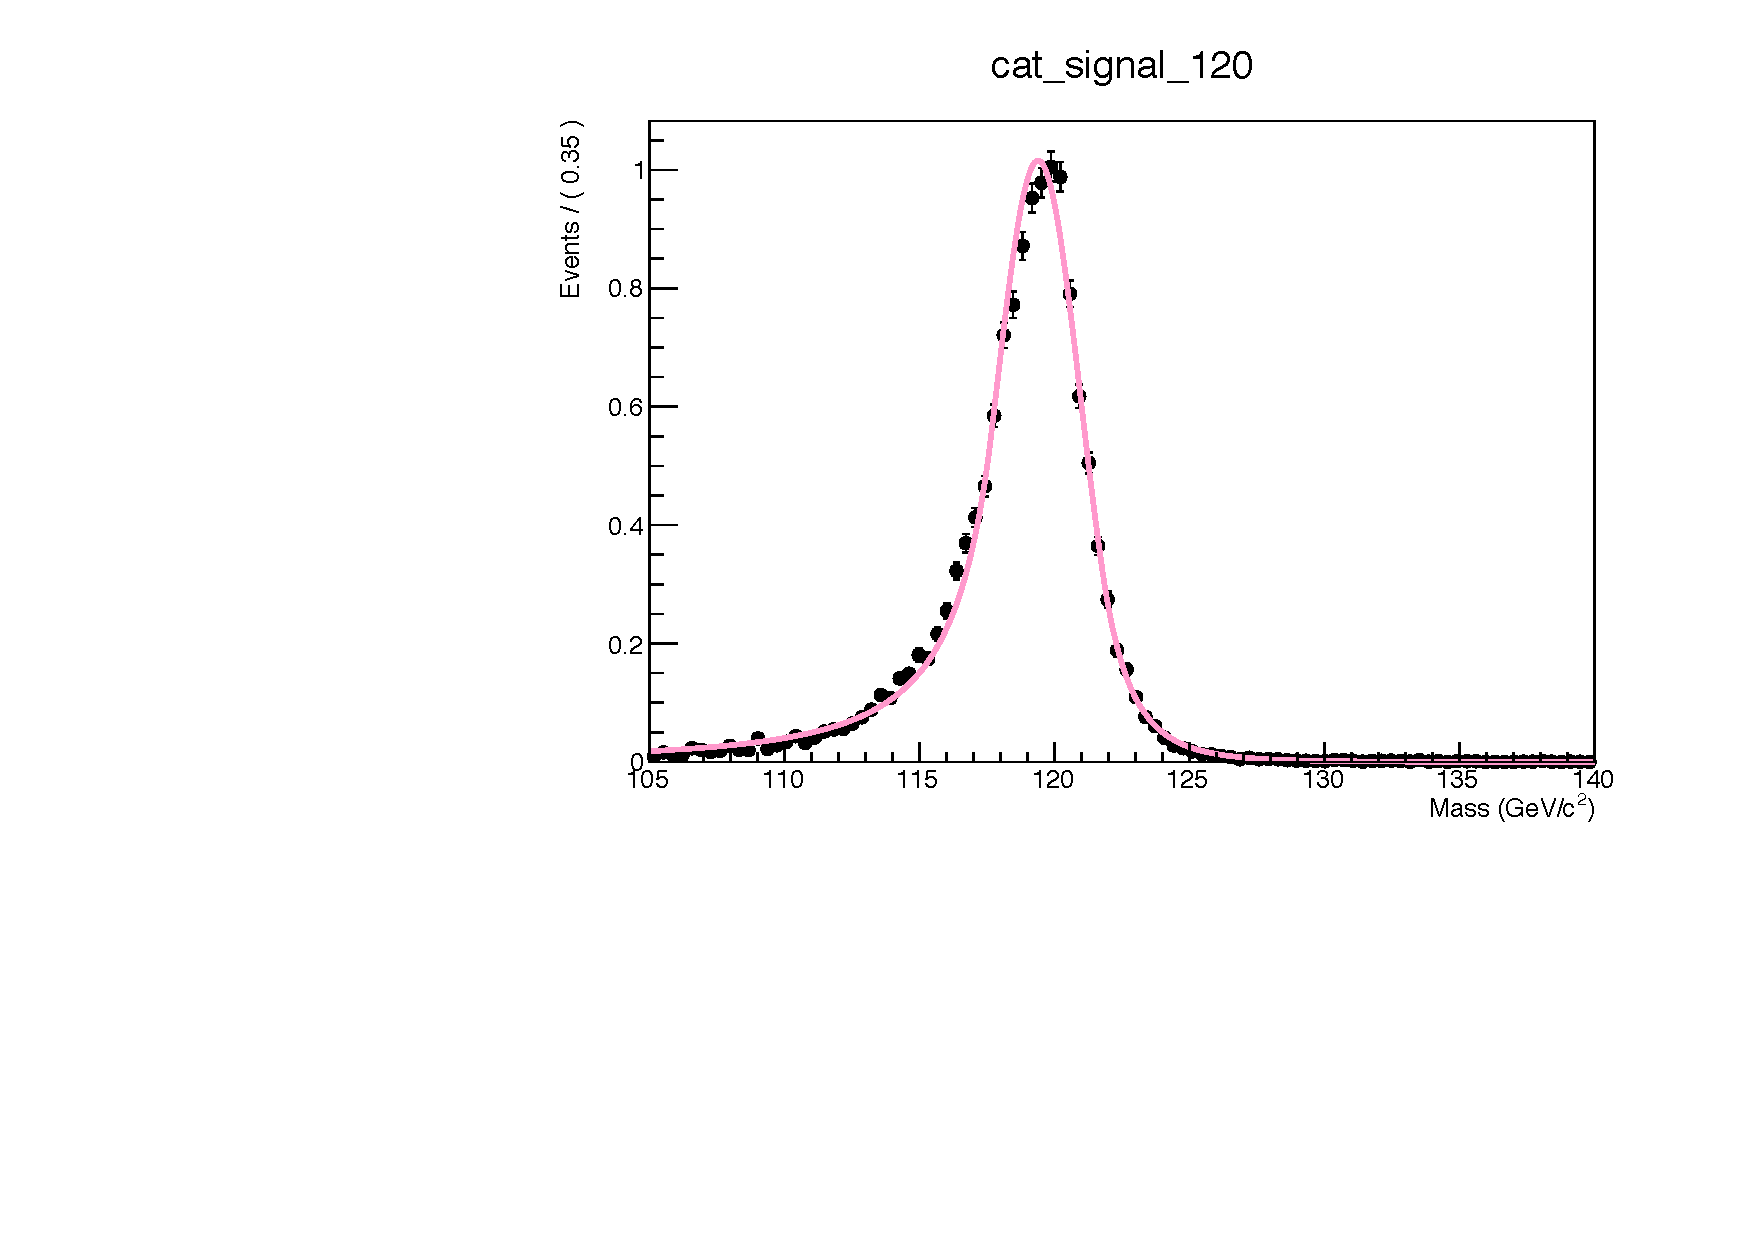
\includegraphics[width=0.3\textwidth]{Figures/SignalModelling/Signal_Parametrization/2016/ggH_2e2mu_2016_120_Sim.pdf}
%	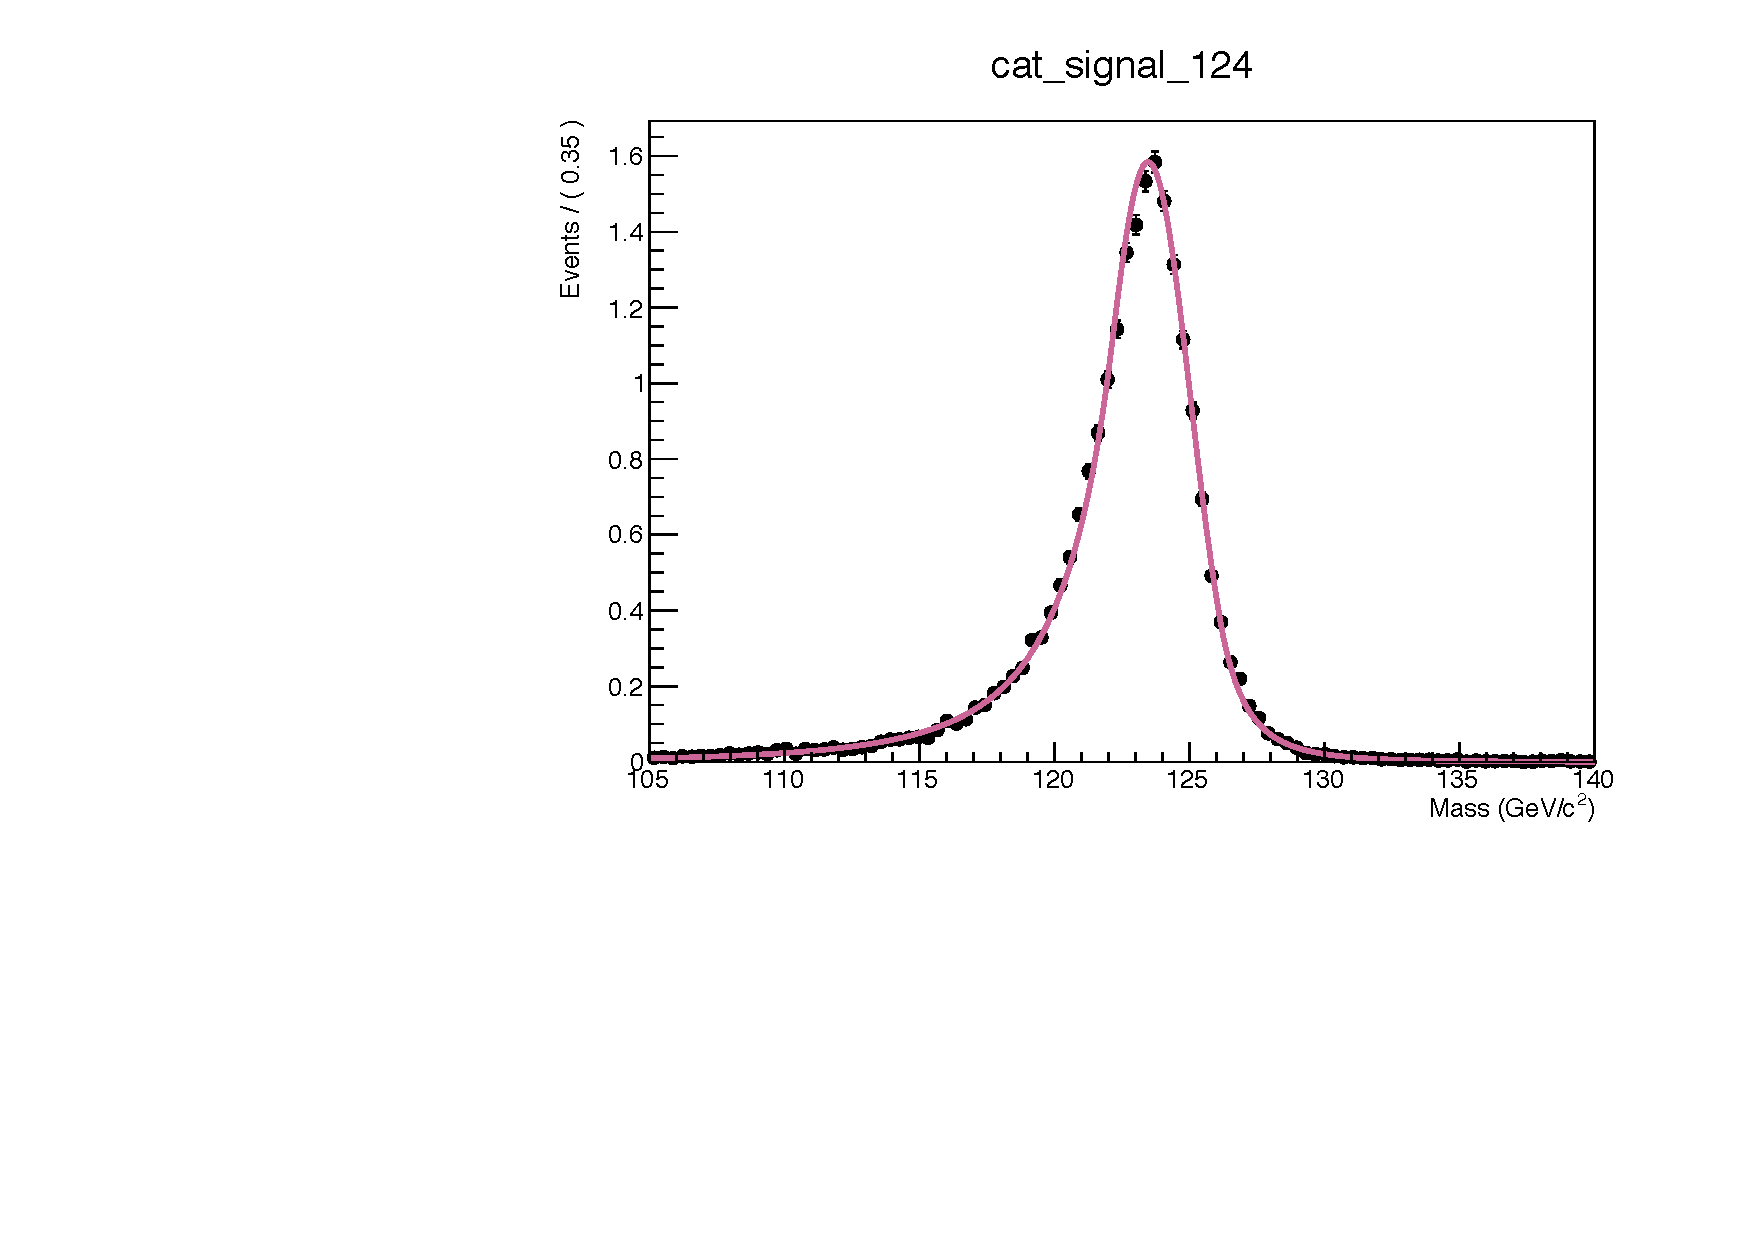
\includegraphics[width=0.3\textwidth]{Figures/SignalModelling/Signal_Parametrization/2016/ggH_2e2mu_2016_124_Sim.pdf} 
%	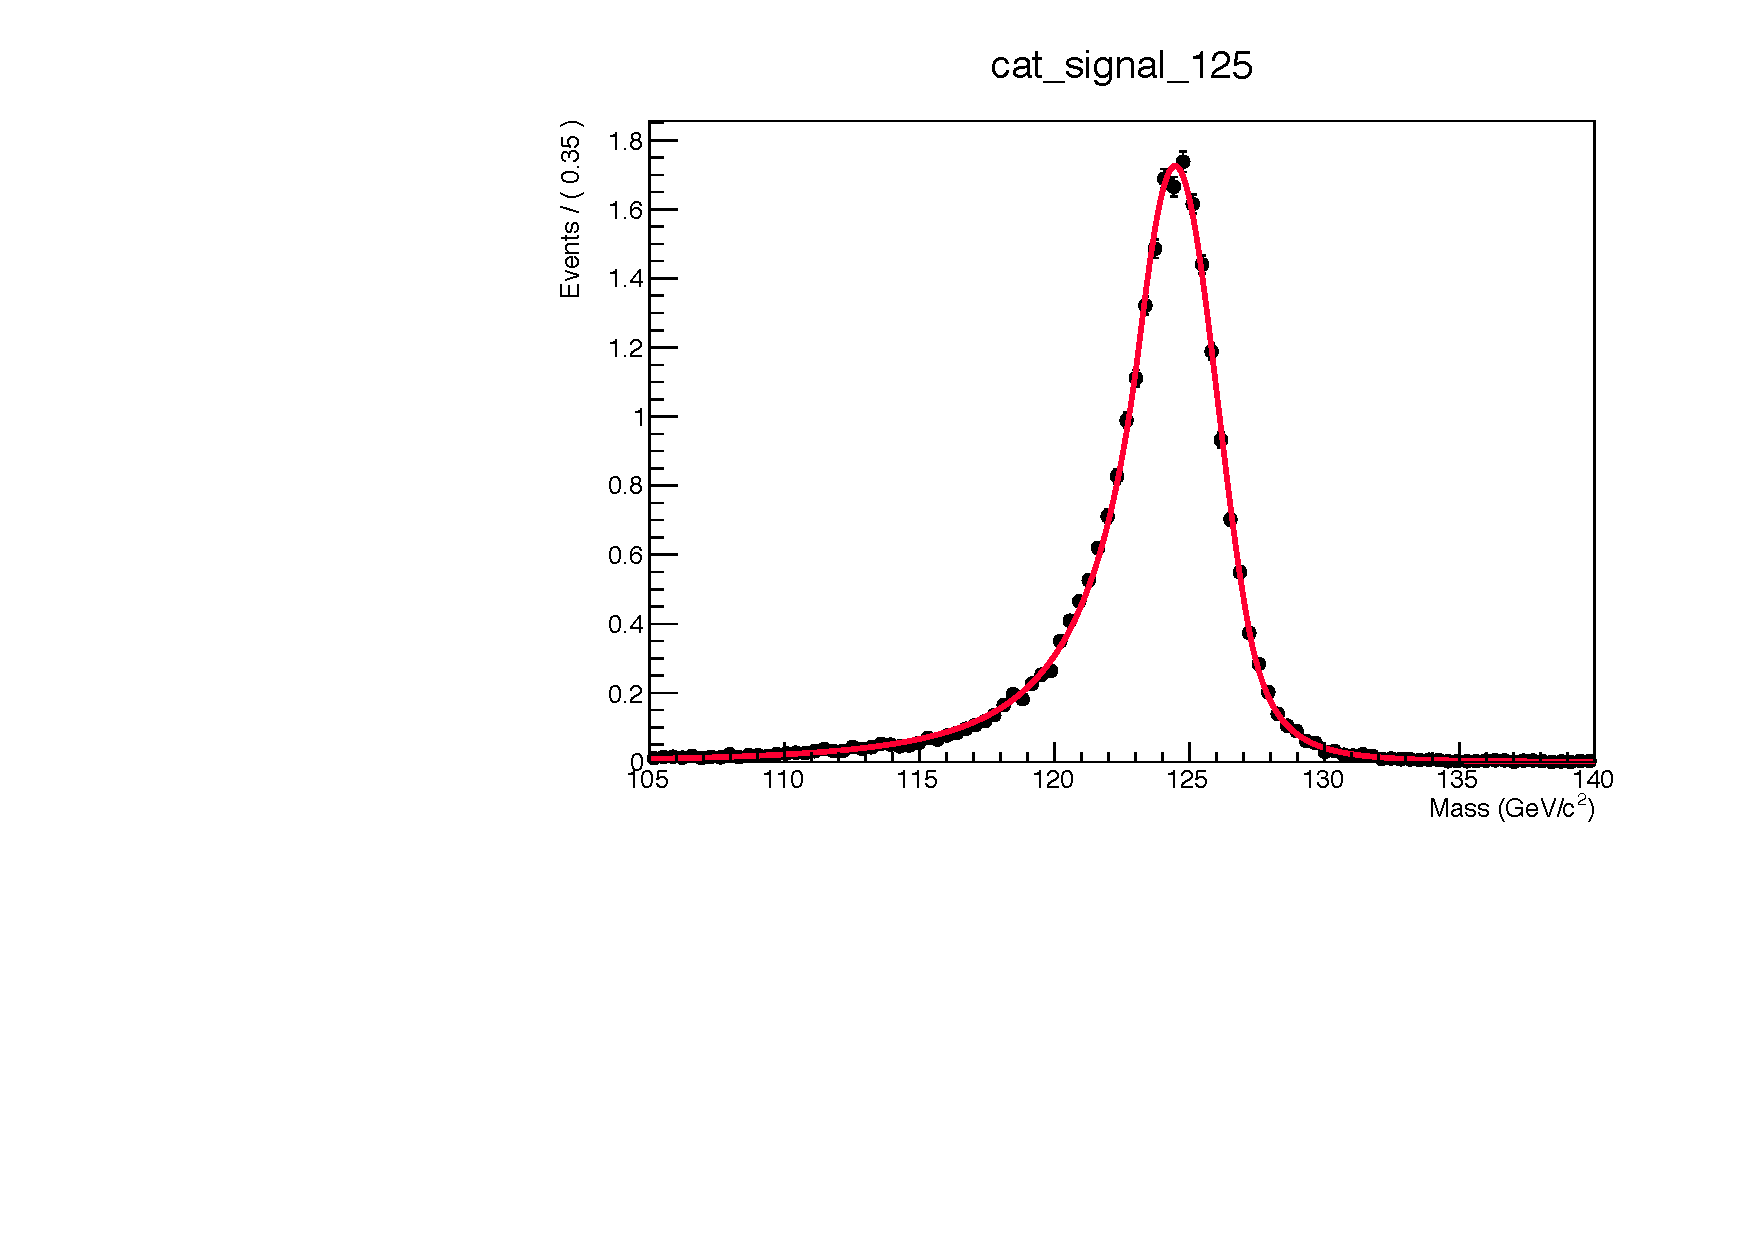
\includegraphics[width=0.3\textwidth]{Figures/SignalModelling/Signal_Parametrization/2016/ggH_2e2mu_2016_125_Sim.pdf}
%		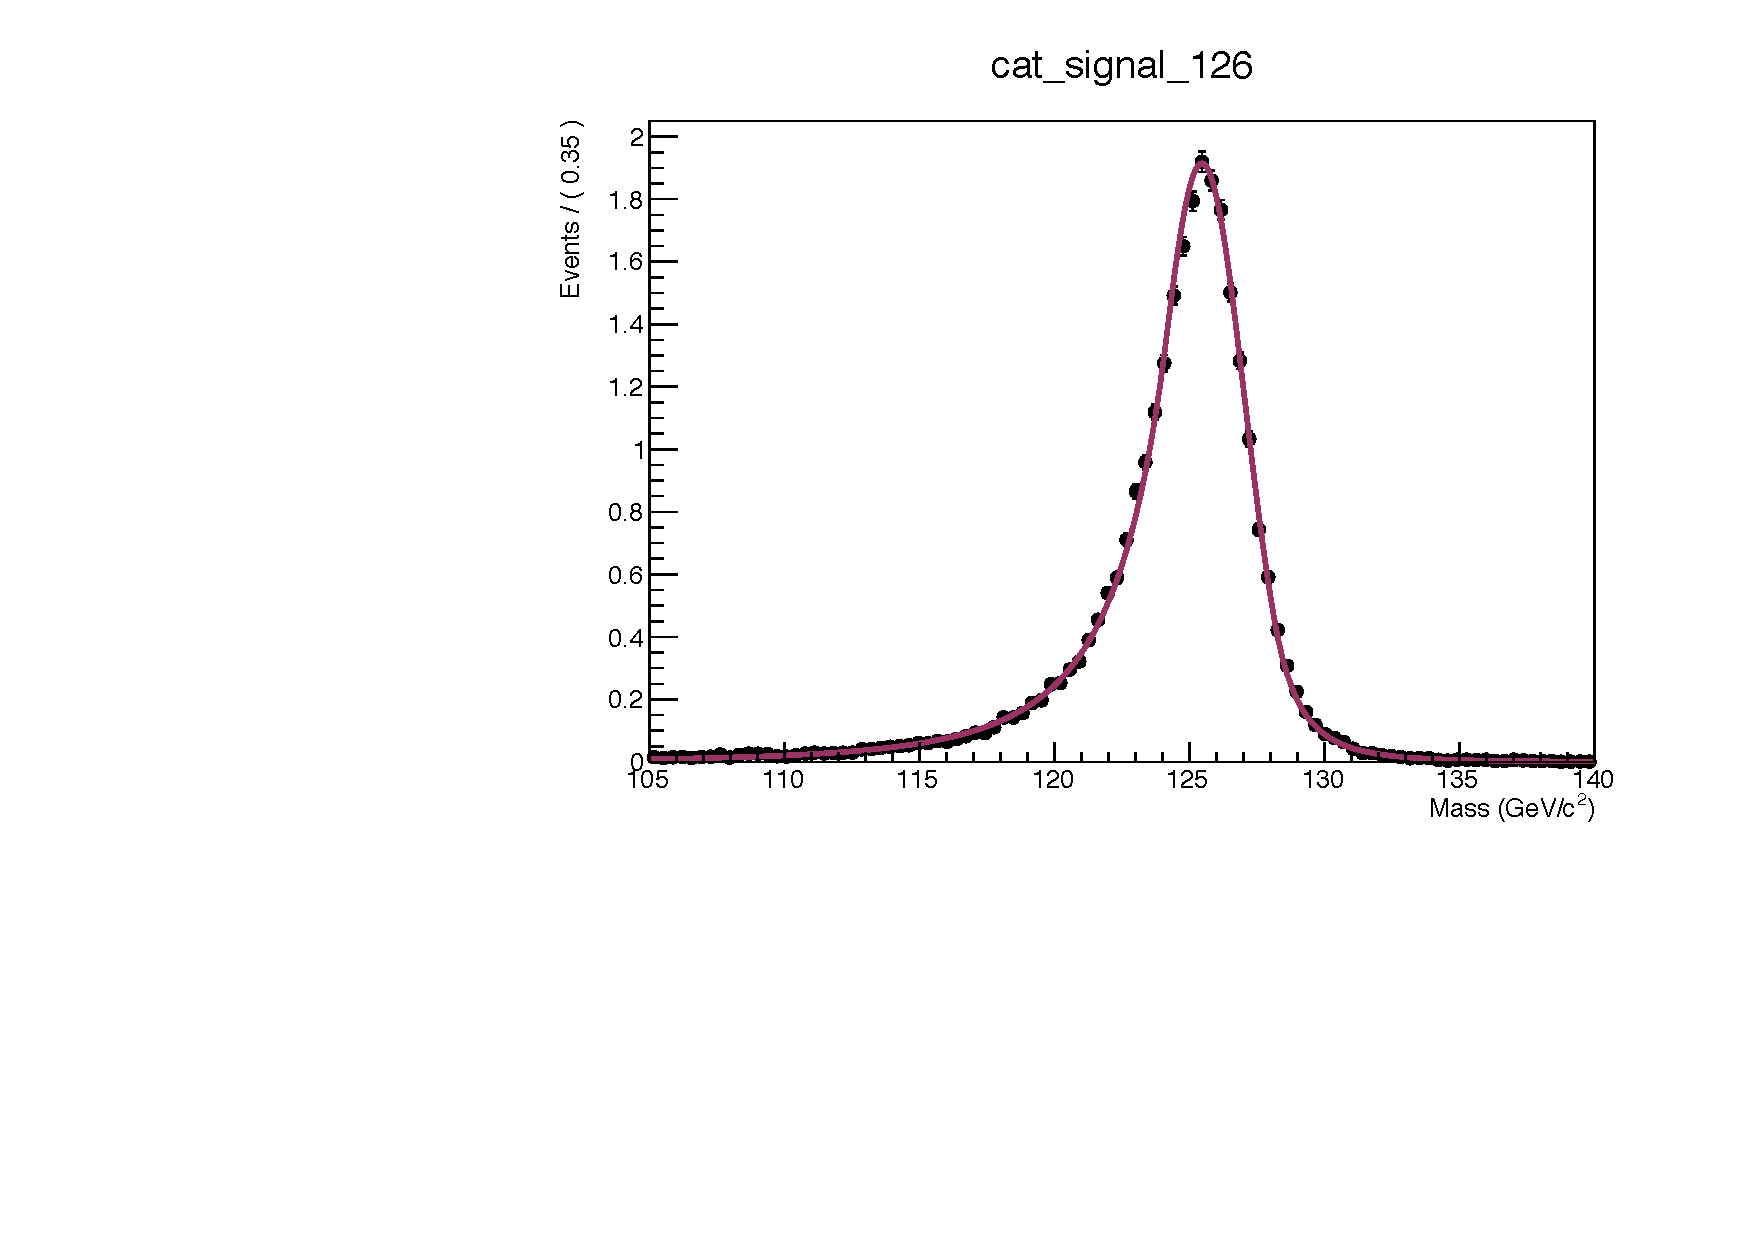
\includegraphics[width=0.3\textwidth]{Figures/SignalModelling/Signal_Parametrization/2016/ggH_2e2mu_2016_126_Sim.pdf}
%		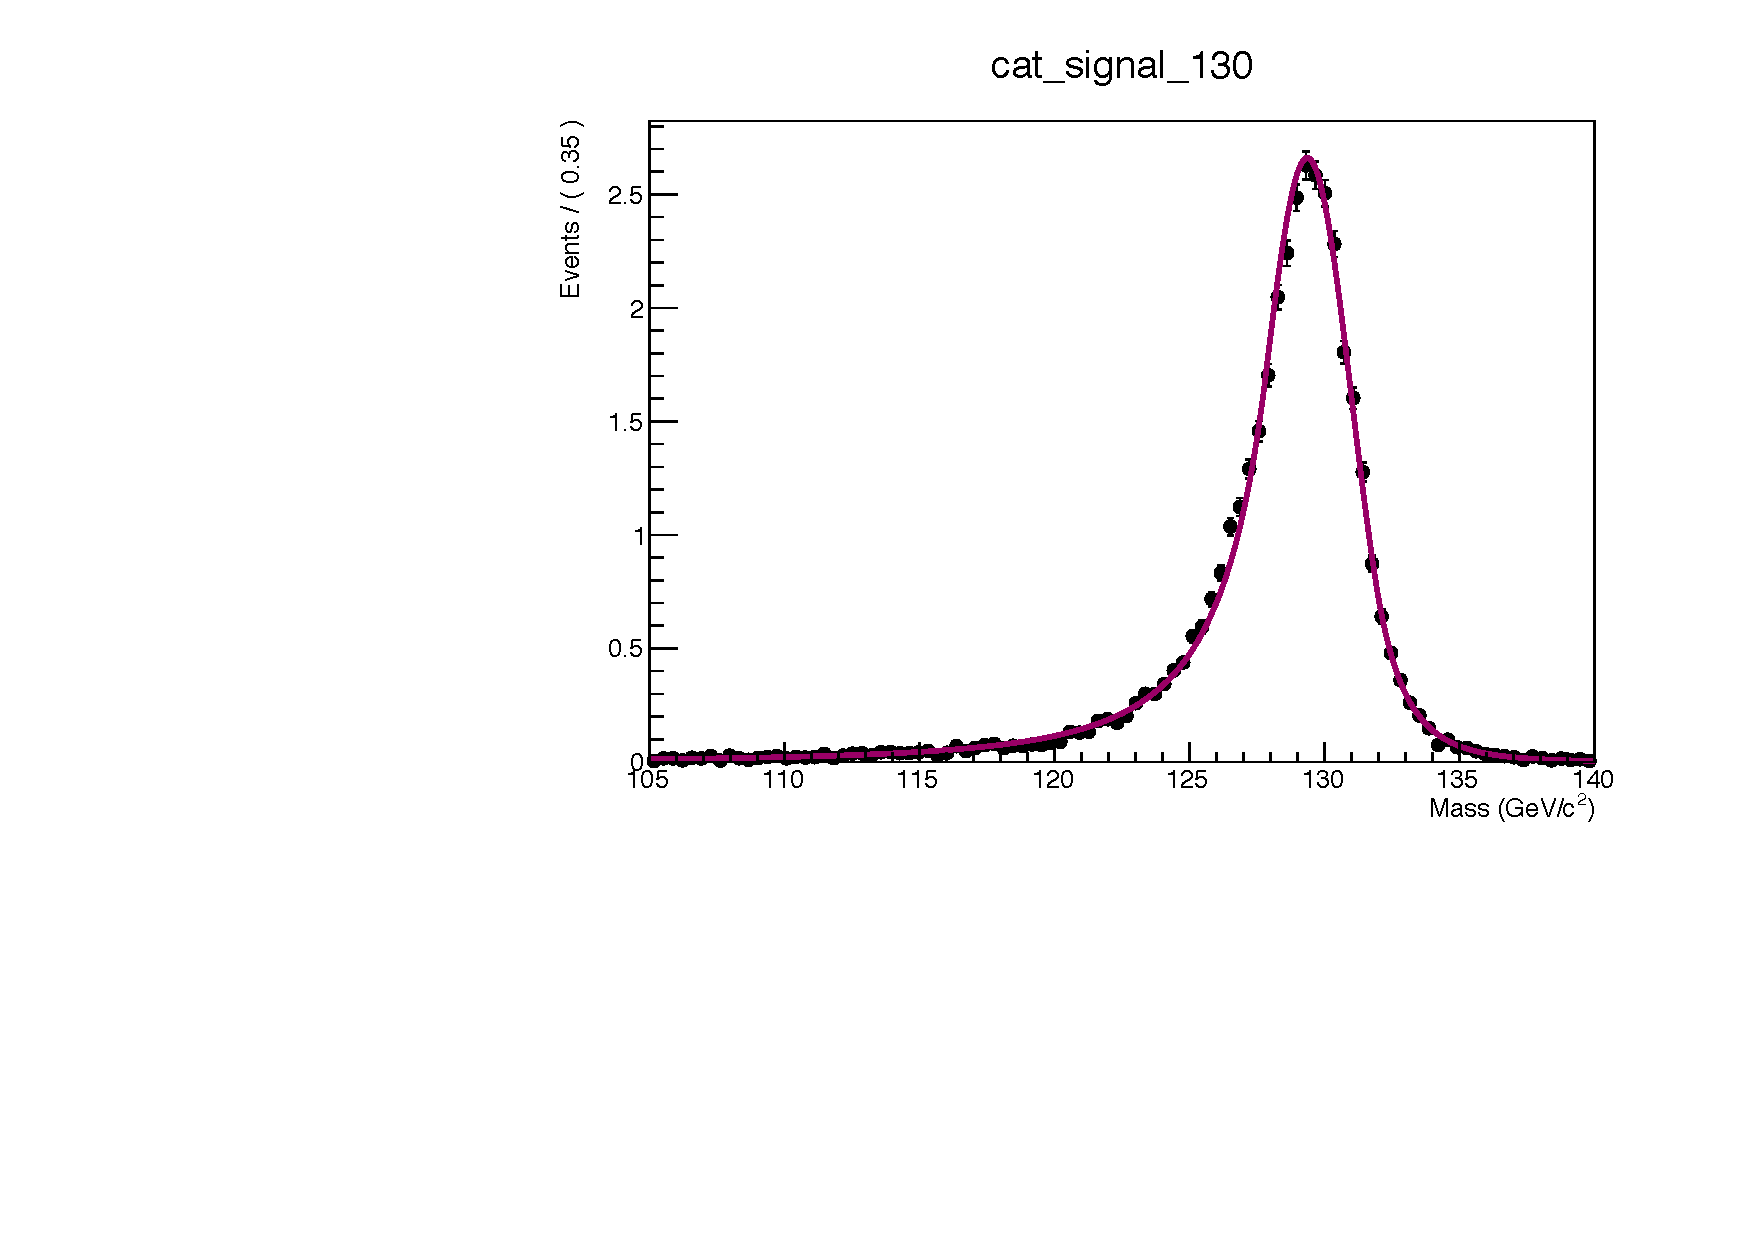
\includegraphics[width=0.3\textwidth]{Figures/SignalModelling/Signal_Parametrization/2016/ggH_2e2mu_2016_130_Sim.pdf}
%		\caption{Simultaneous fit for ggH production mode, in 2016, for different mass points, 
%		in 2e2$\mu$ final state.}
%	\label{signal_lineshape_2016_full_1}
%	\end{center}
%\end{figure}
%\begin{figure}[!htbp]
%	\begin{center}
%   		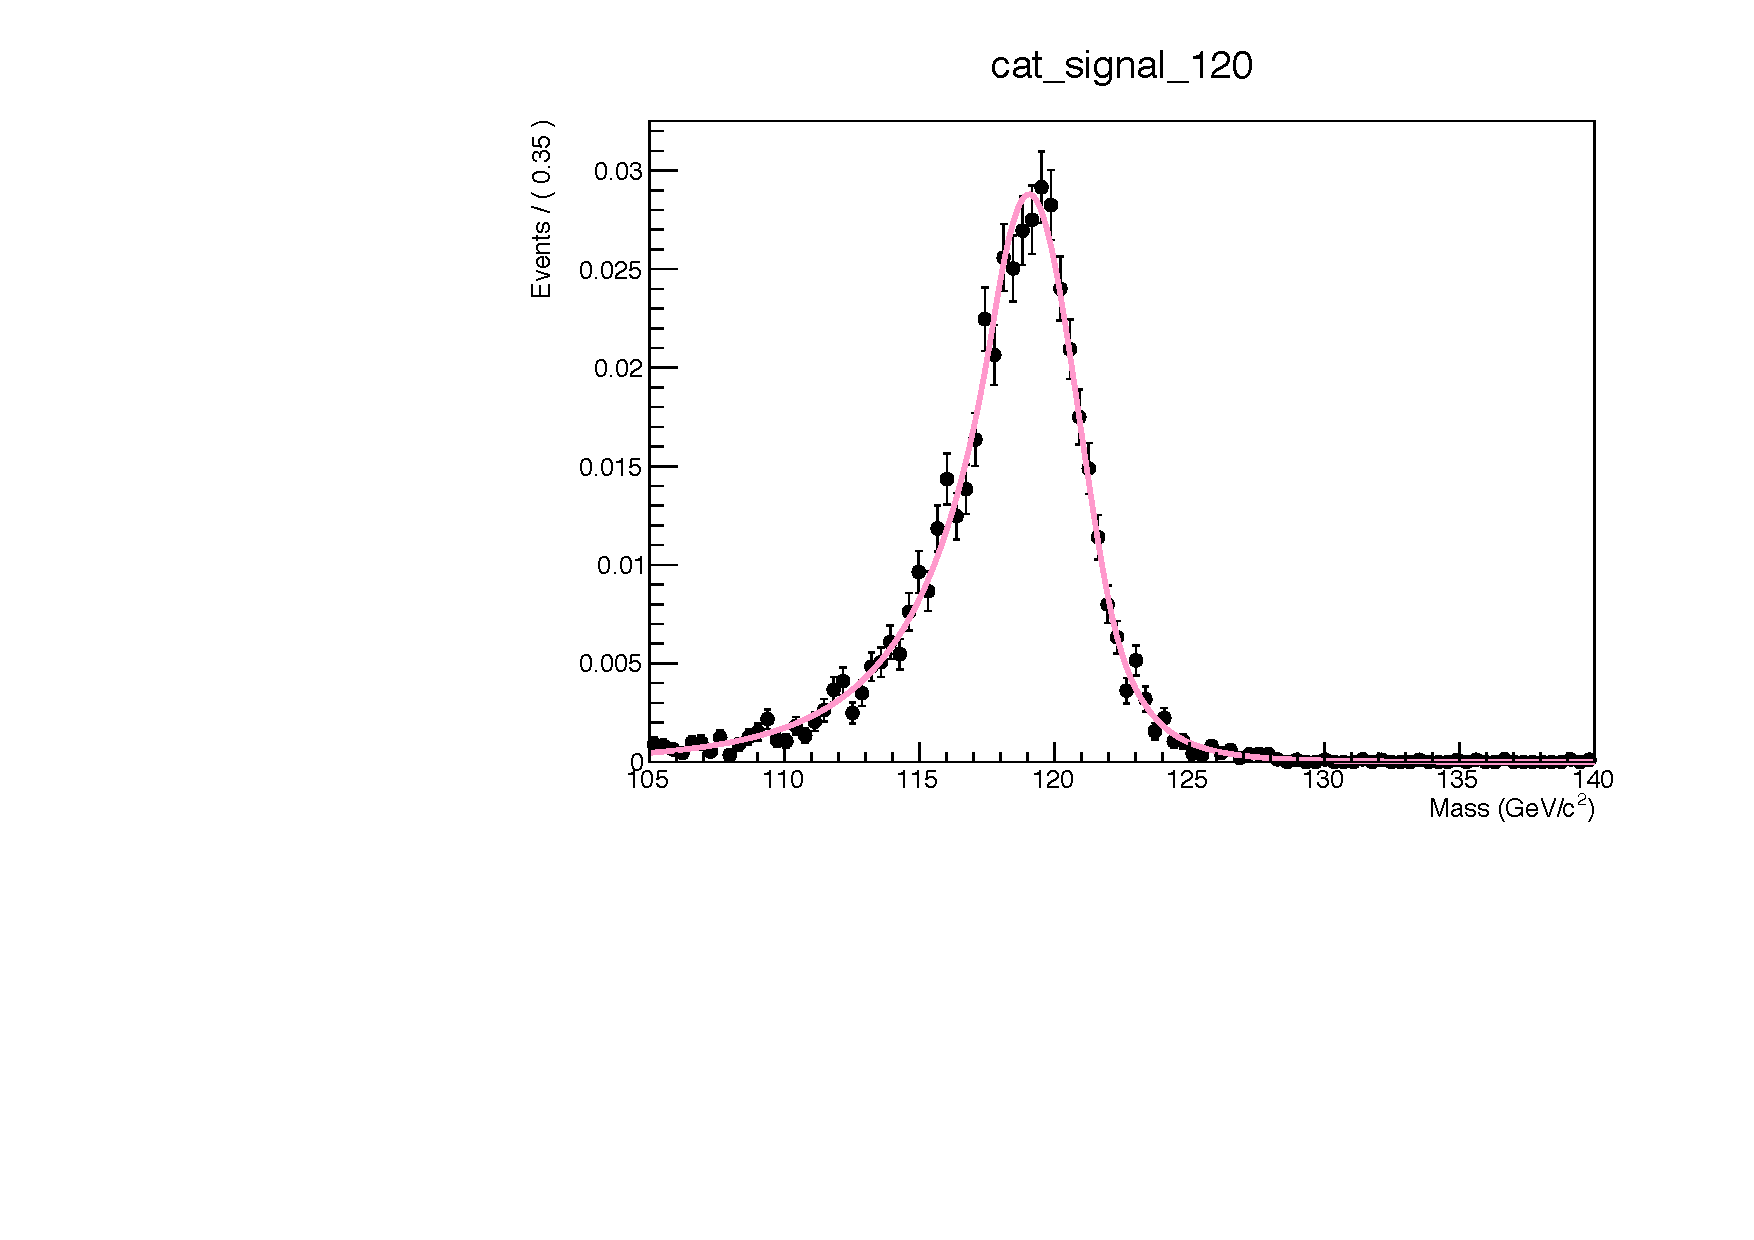
\includegraphics[width=0.3\textwidth]{Figures/SignalModelling/Signal_Parametrization/2016/VBF_4e_2016_120_Sim.pdf}
%		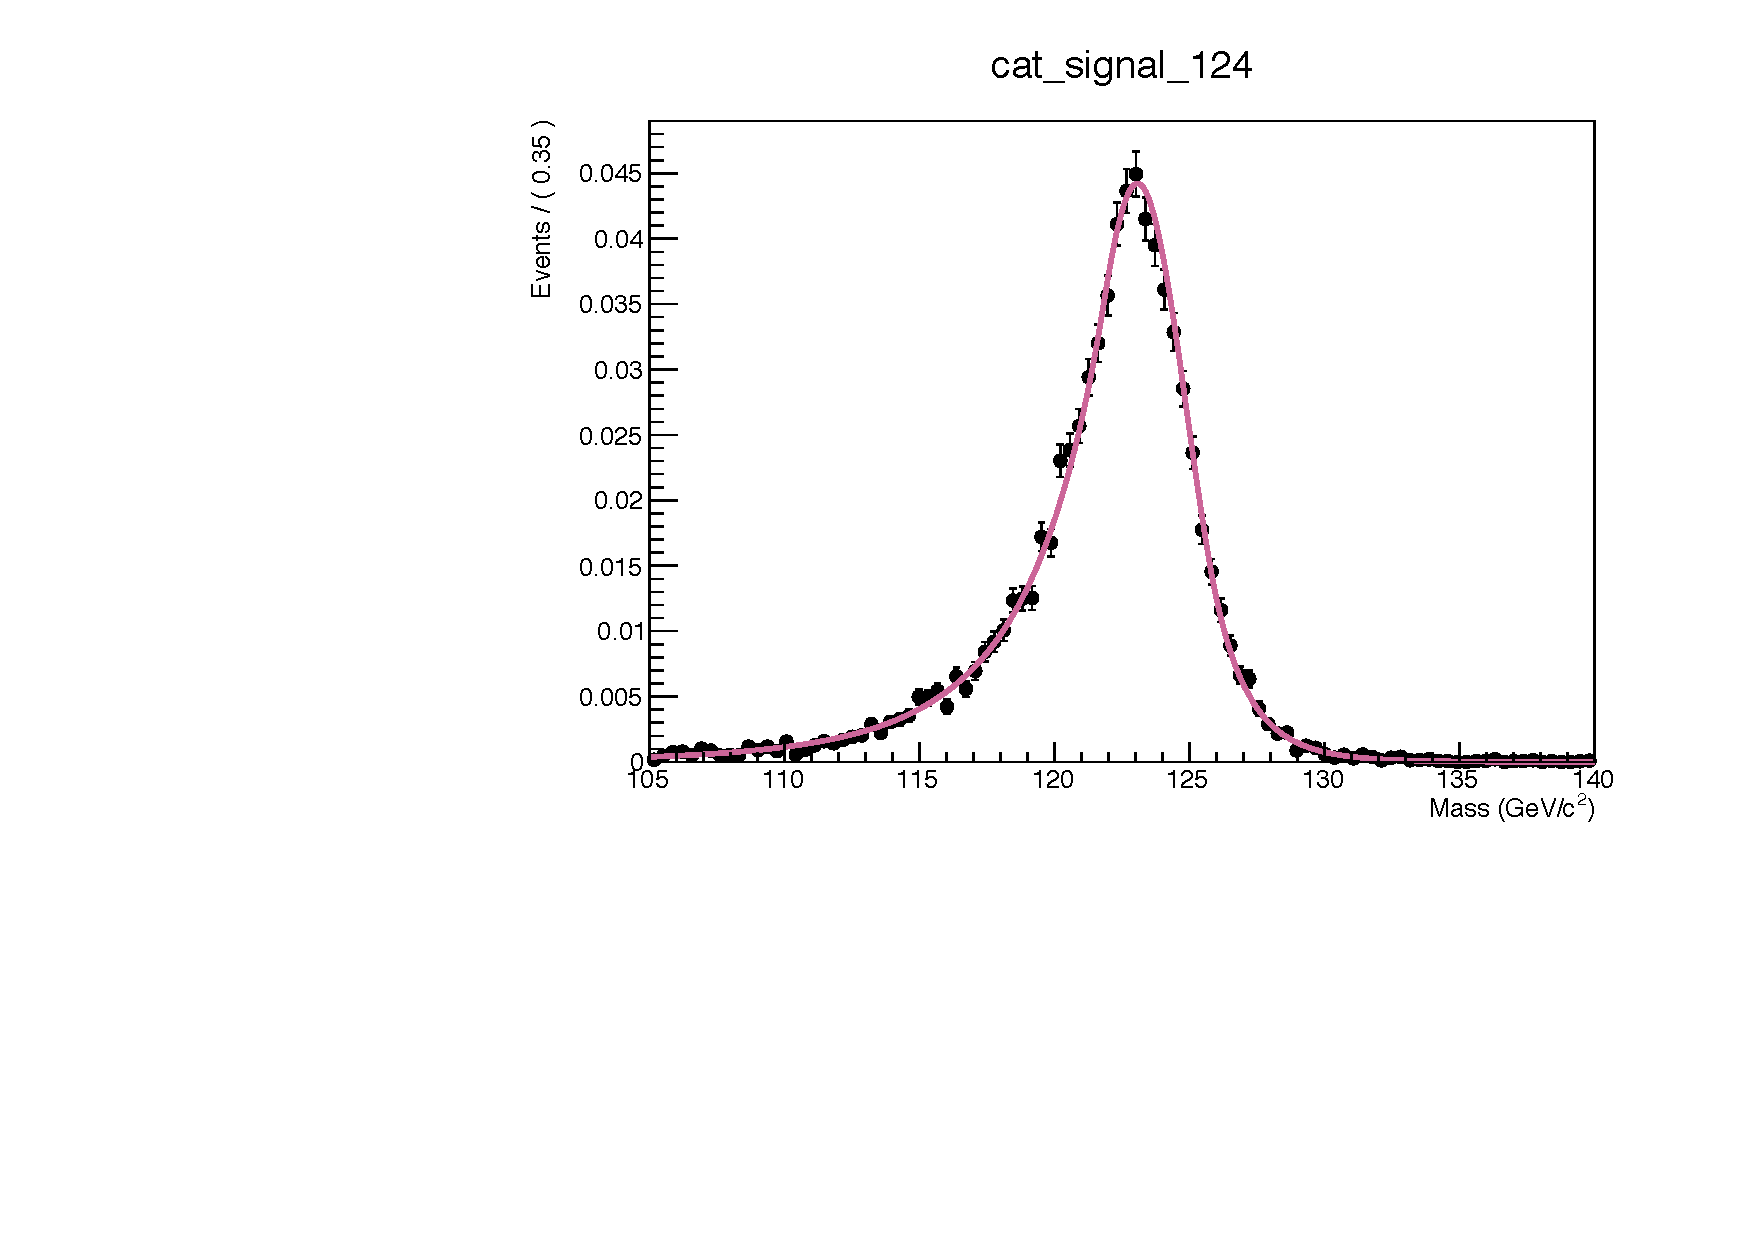
\includegraphics[width=0.3\textwidth]{Figures/SignalModelling/Signal_Parametrization/2016/VBF_4e_2016_124_Sim.pdf} 
%		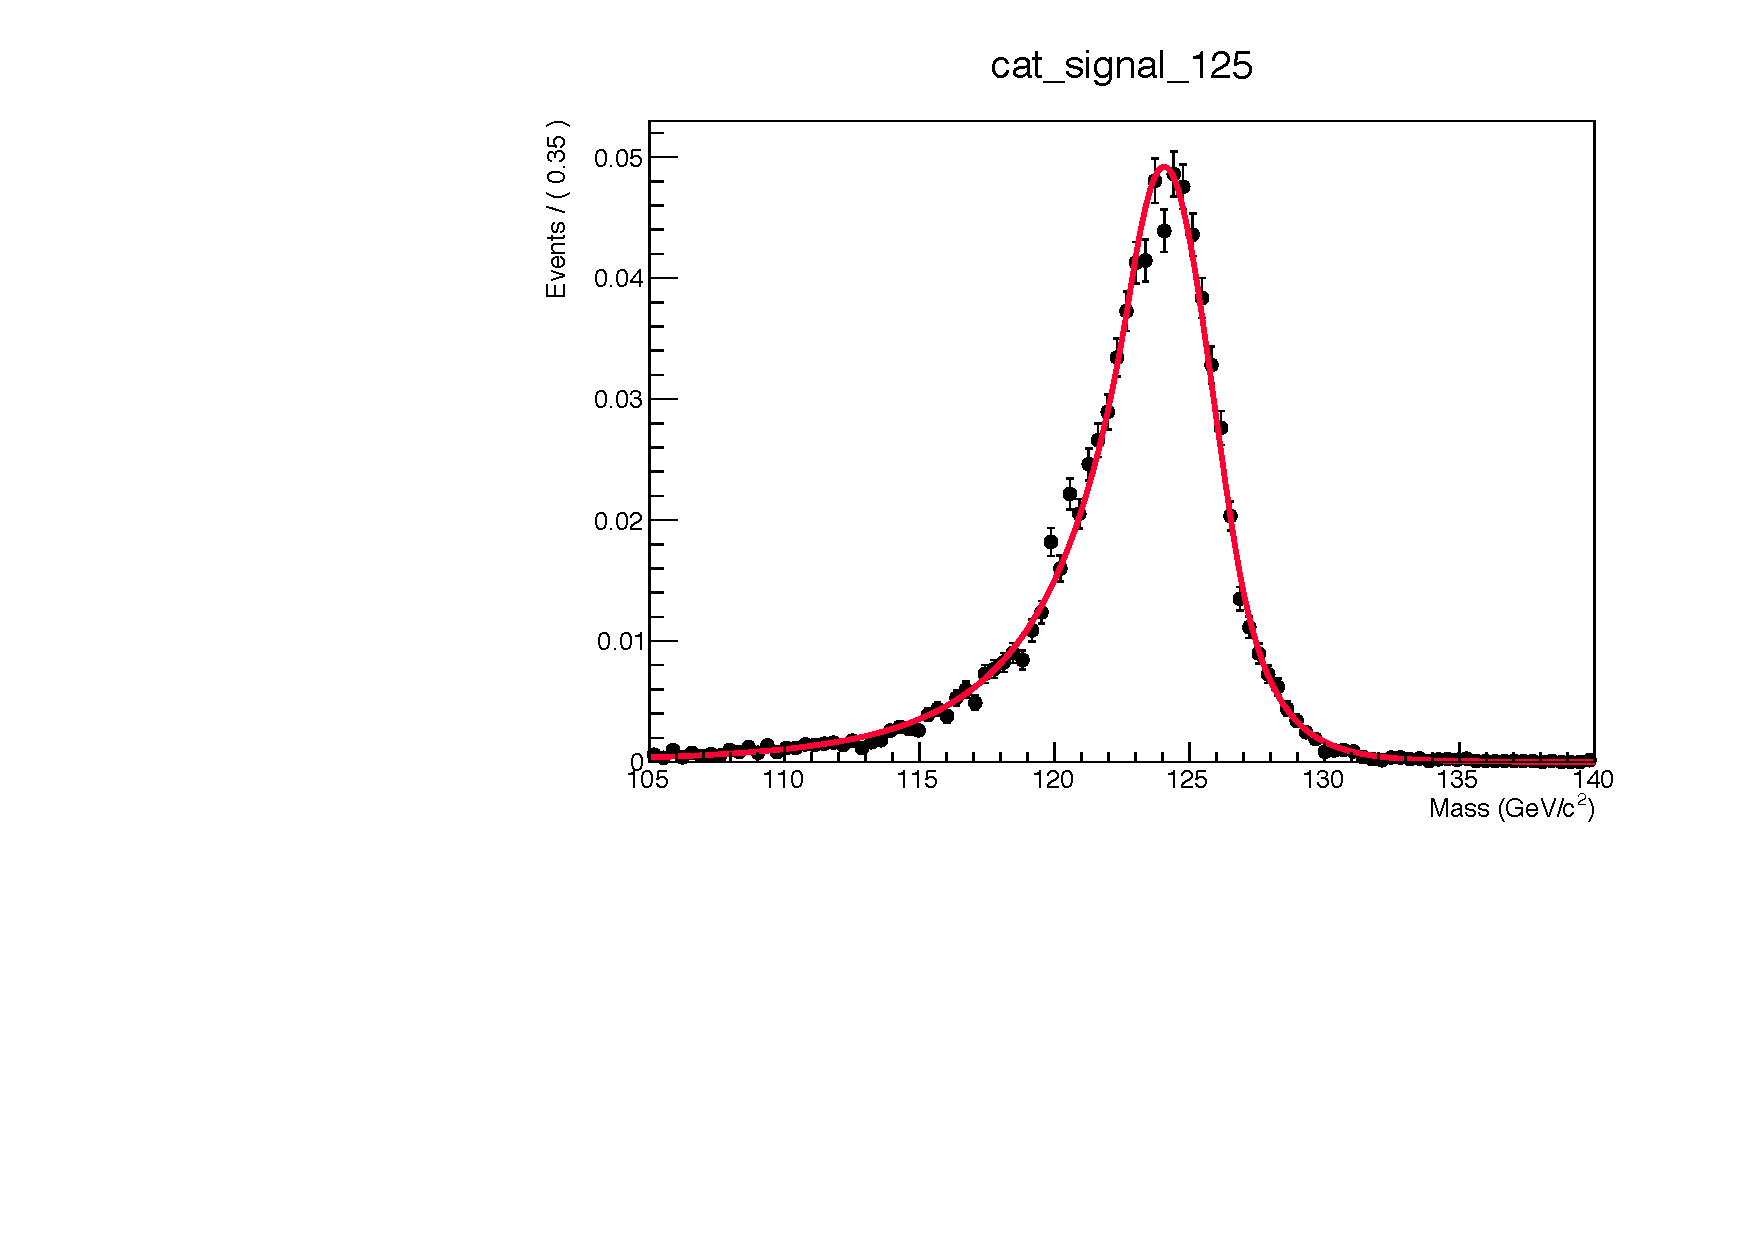
\includegraphics[width=0.3\textwidth]{Figures/SignalModelling/Signal_Parametrization/2016/VBF_4e_2016_125_Sim.pdf}
%		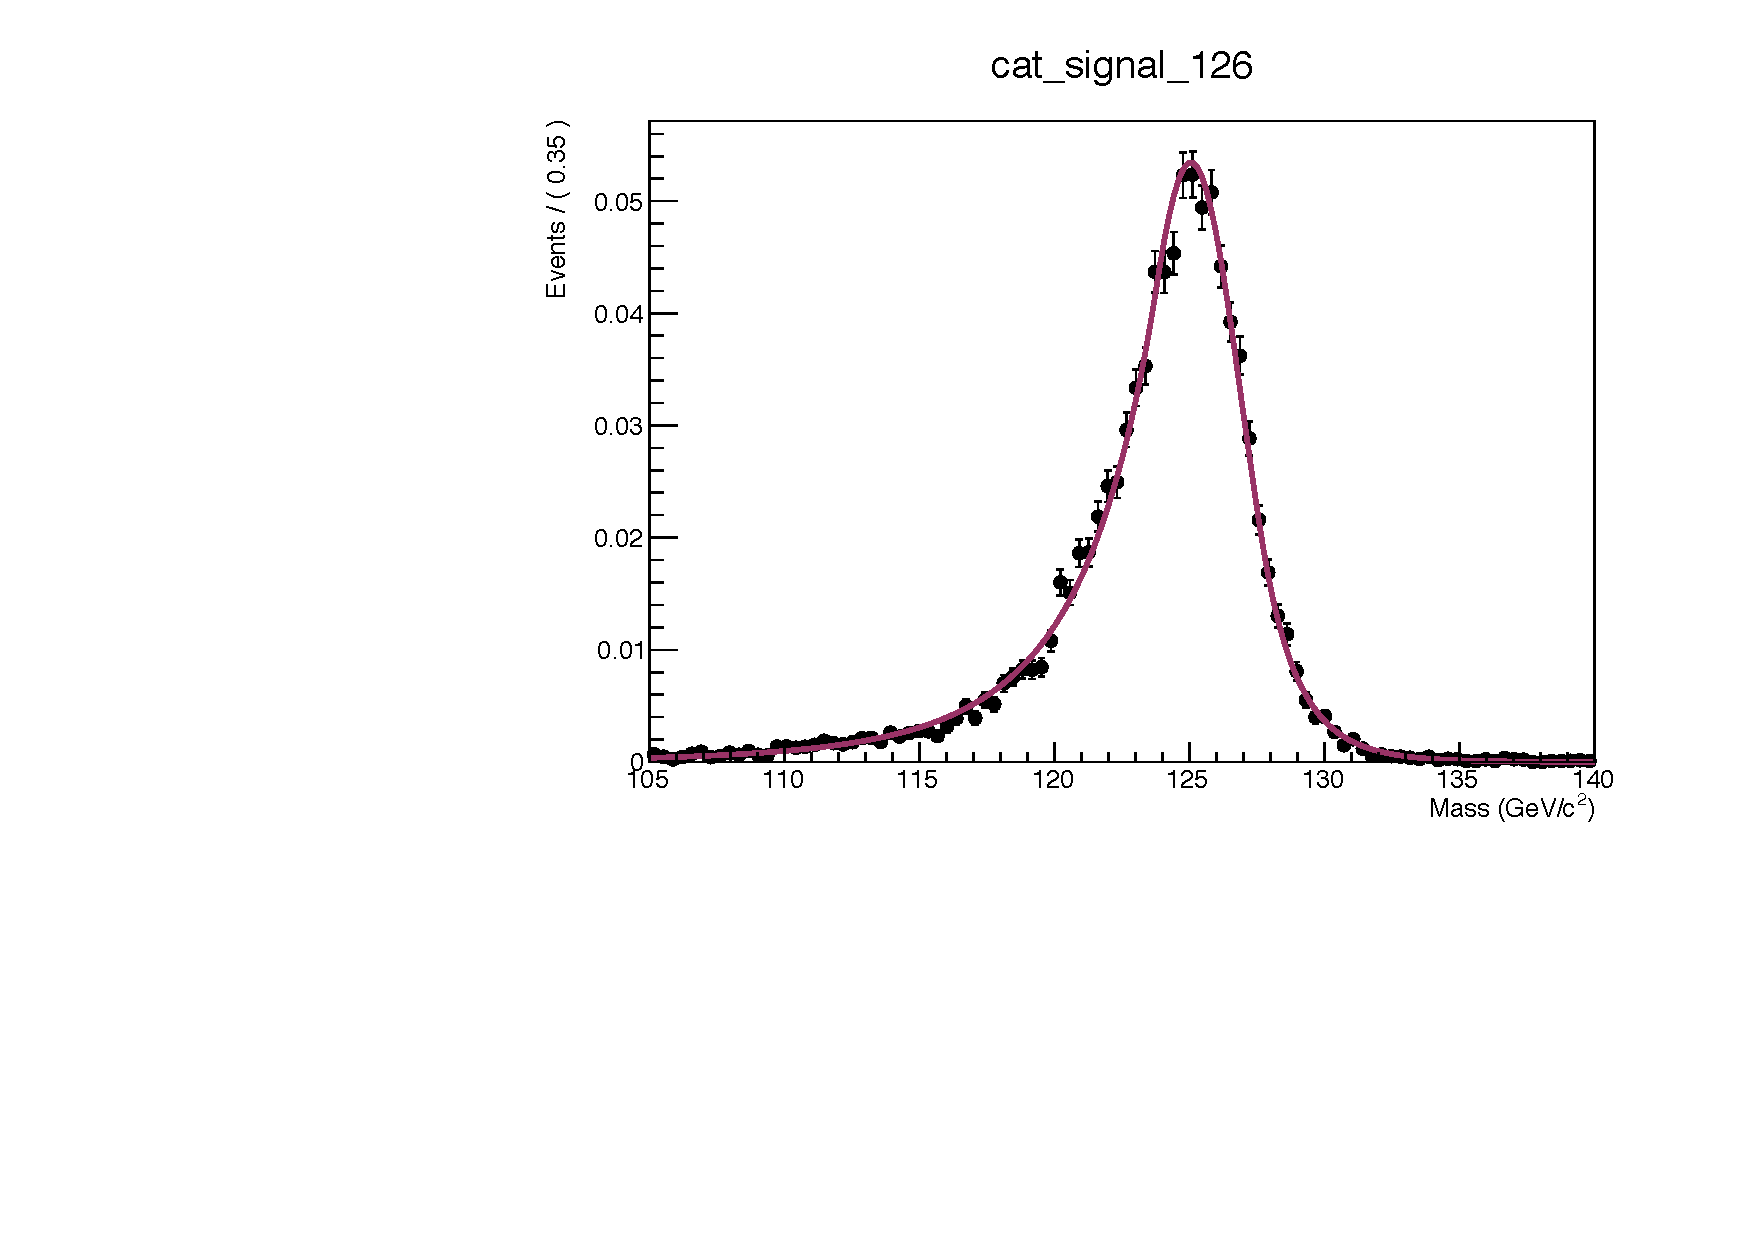
\includegraphics[width=0.3\textwidth]{Figures/SignalModelling/Signal_Parametrization/2016/VBF_4e_2016_126_Sim.pdf}
%		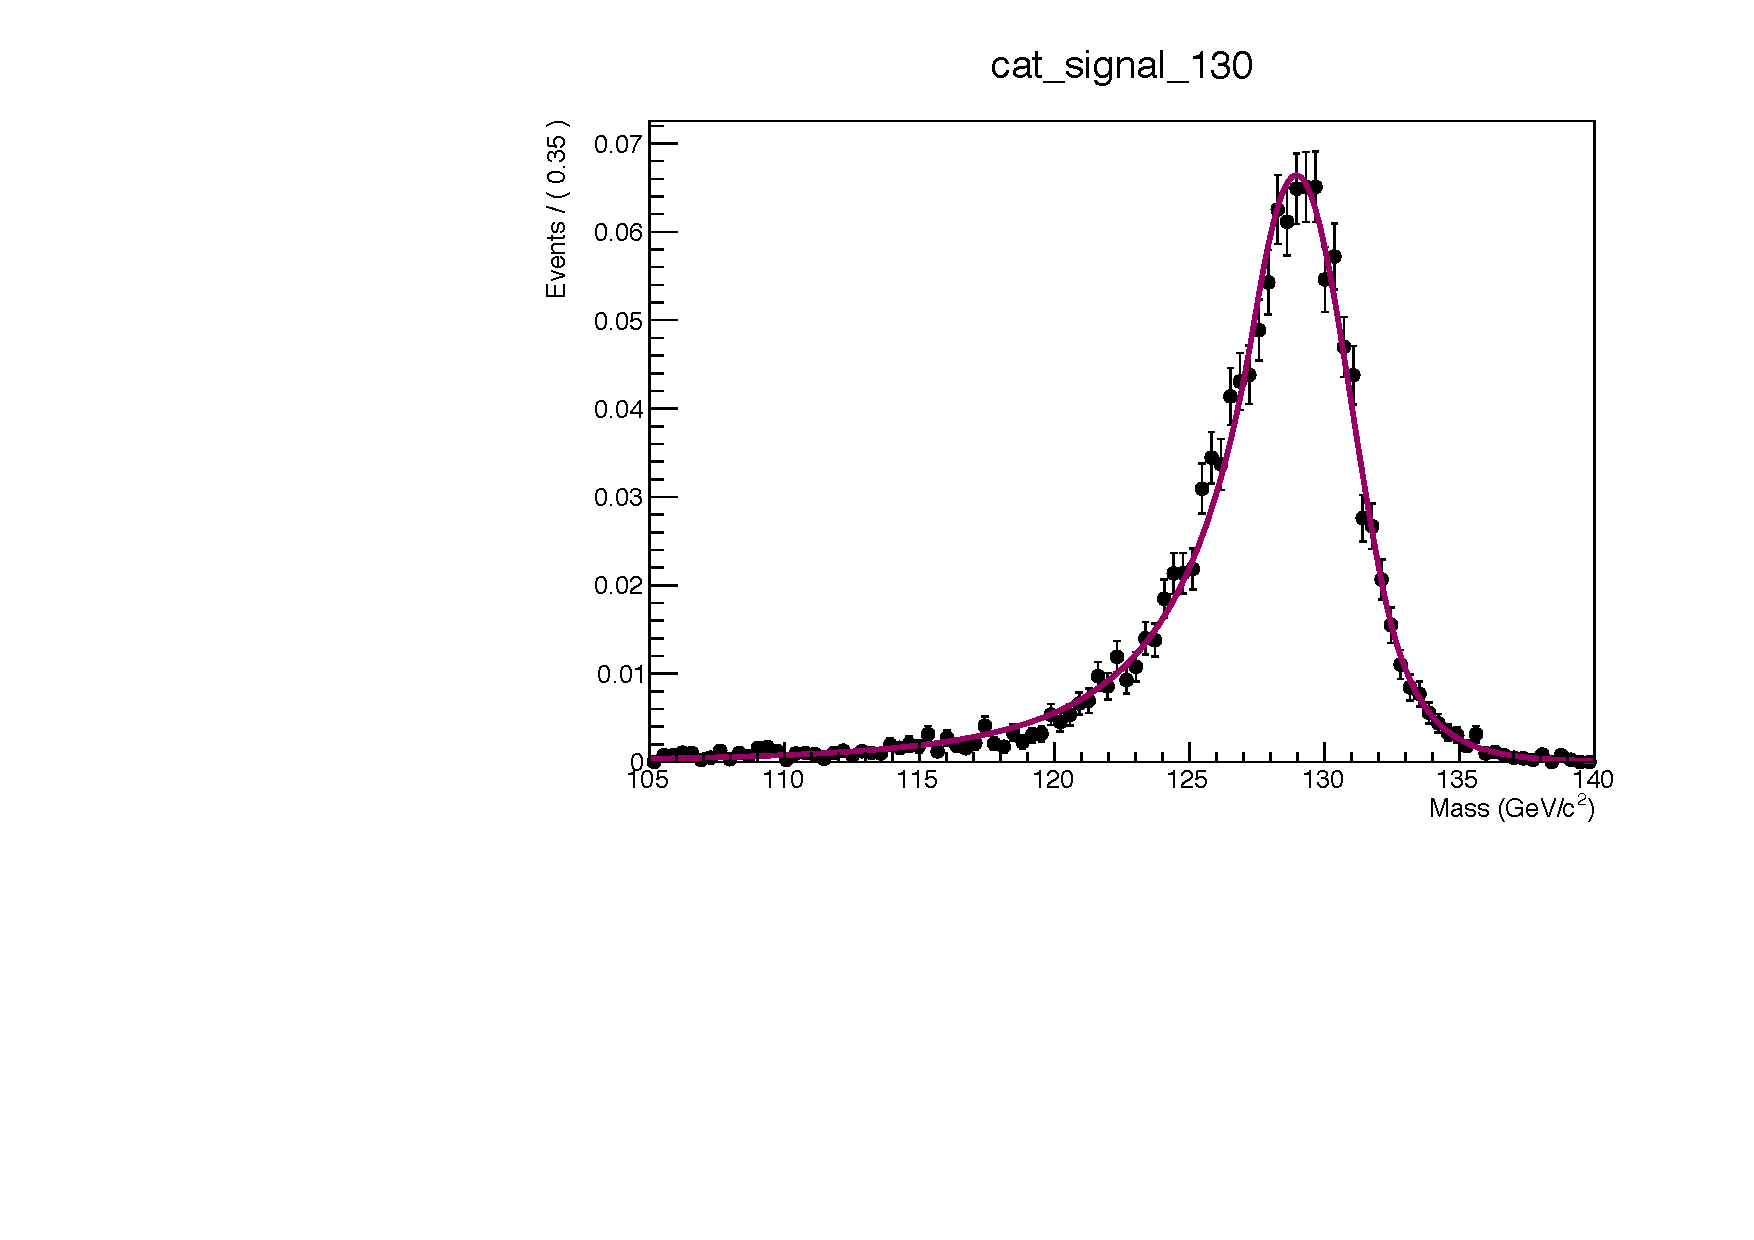
\includegraphics[width=0.3\textwidth]{Figures/SignalModelling/Signal_Parametrization/2016/VBF_4e_2016_130_Sim.pdf}
%		\caption{Simultaneous fit for VBF production mode, in 2016, for different mass points, 
%		in 4e final state.}
%	\label{signal_lineshape_2016_full_2}
%	\end{center}
%\end{figure}
%\begin{figure}[!htbp]
%	\begin{center}
%		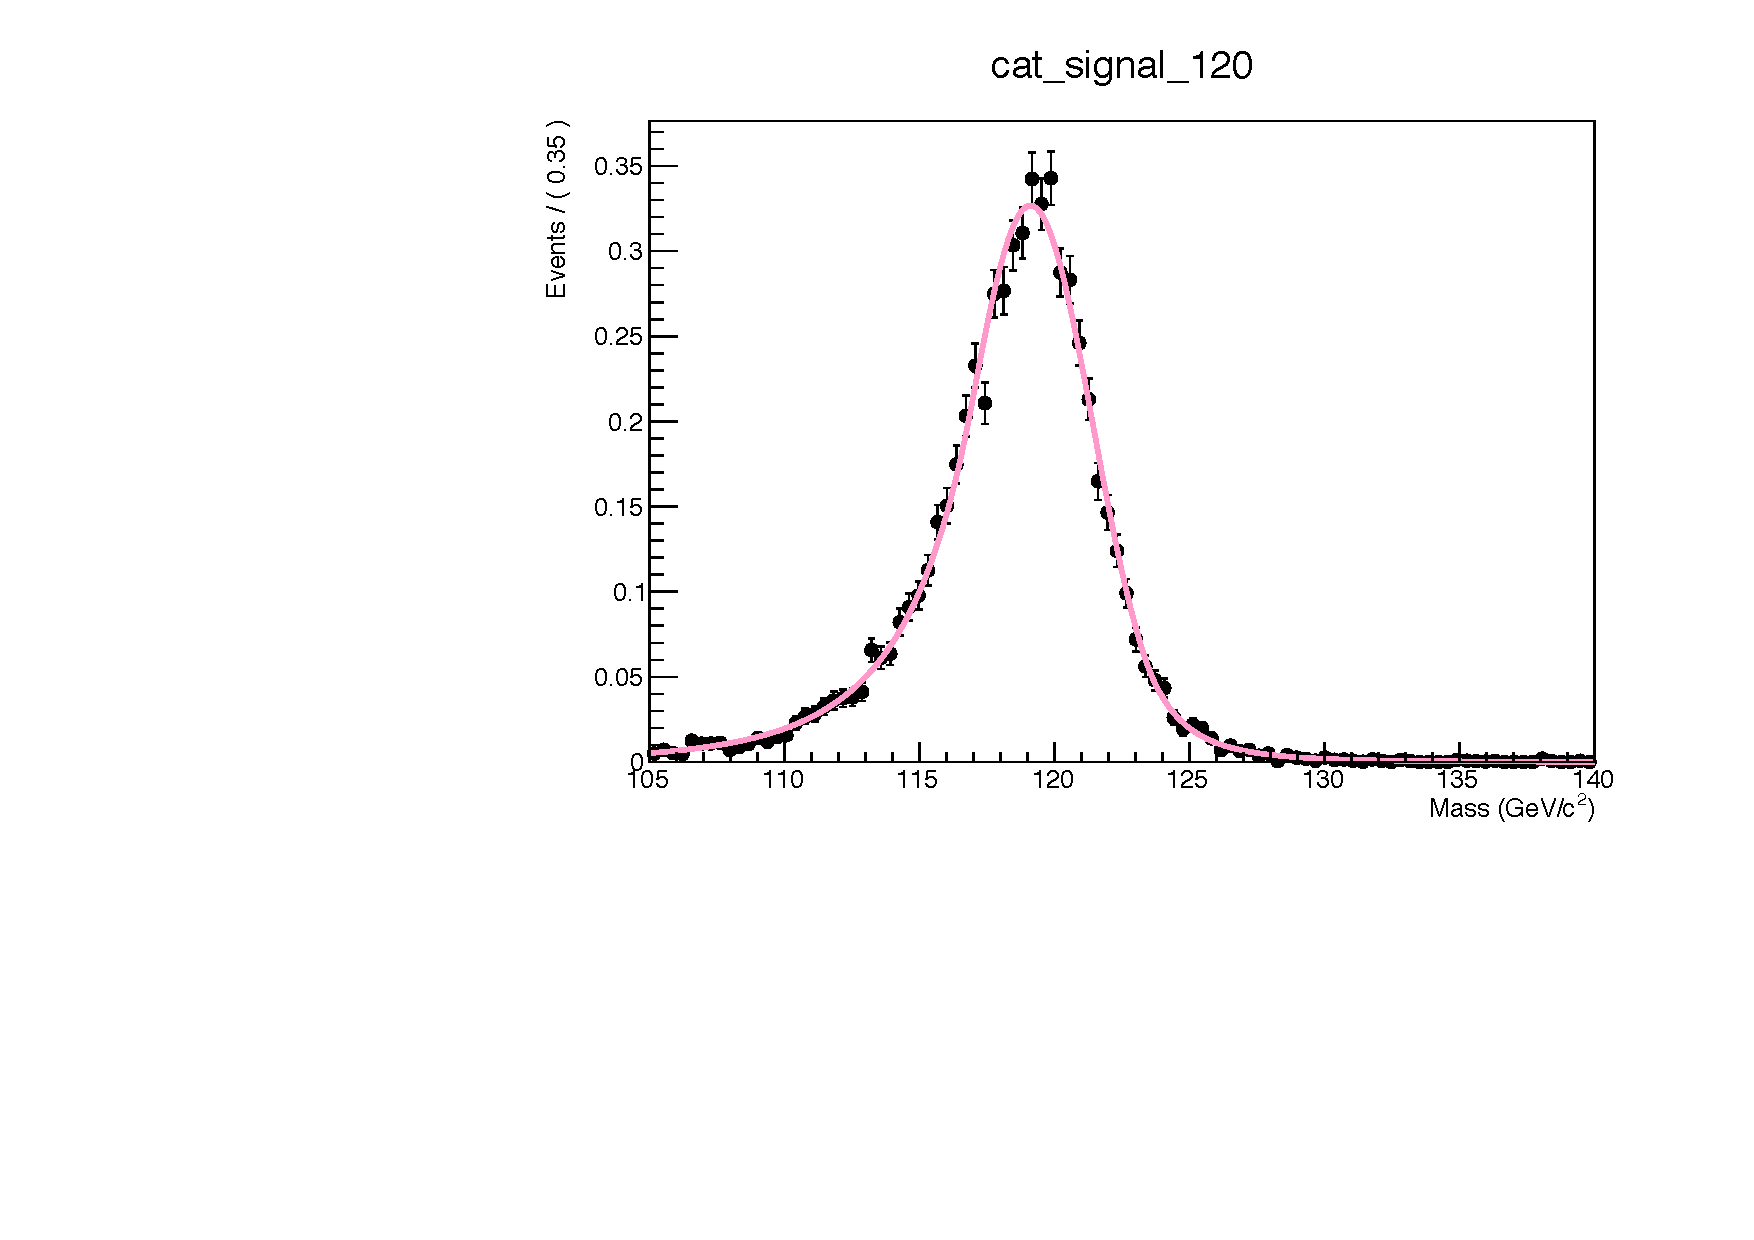
\includegraphics[width=0.3\textwidth]{Figures/SignalModelling/Signal_Parametrization/2017/ggH_4e_2017_120_Sim.pdf}
%		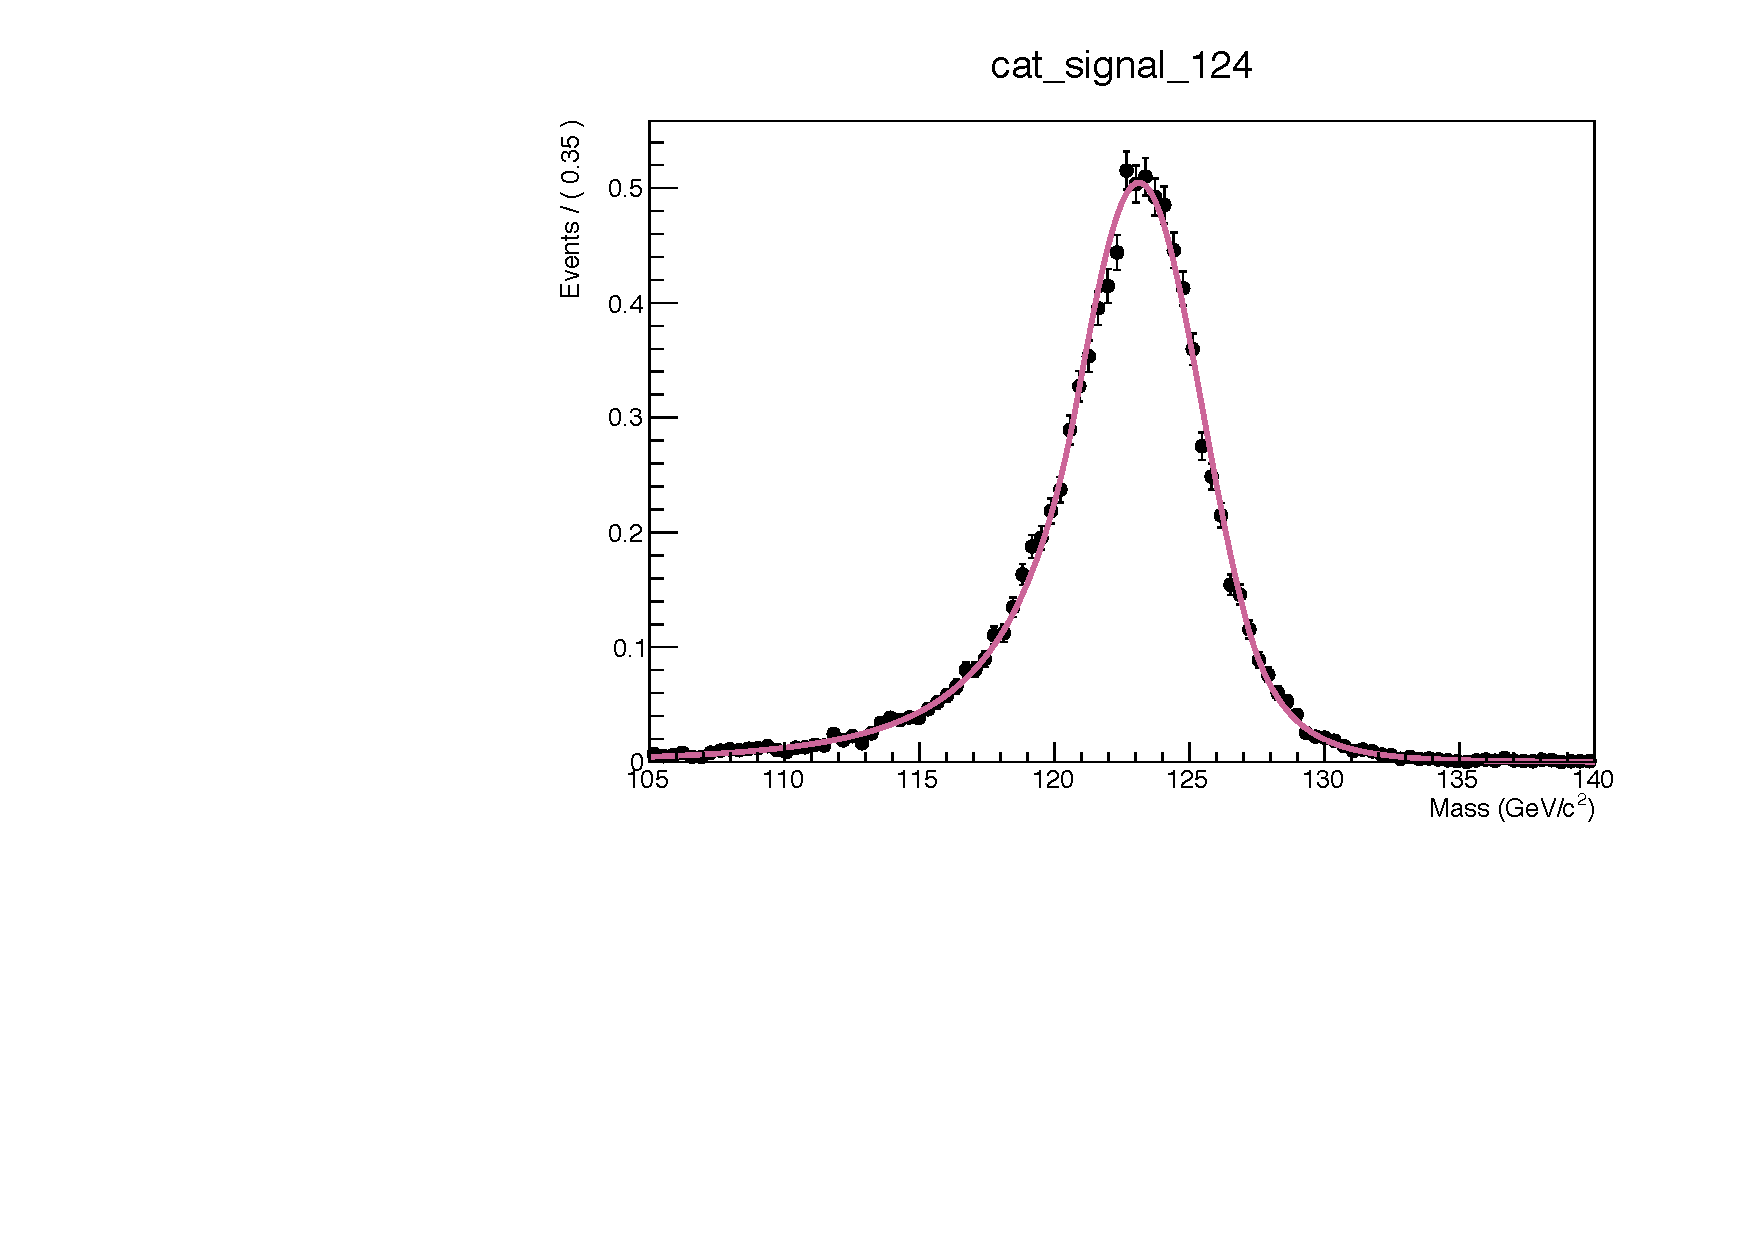
\includegraphics[width=0.3\textwidth]{Figures/SignalModelling/Signal_Parametrization/2017/ggH_4e_2017_124_Sim.pdf}
%   		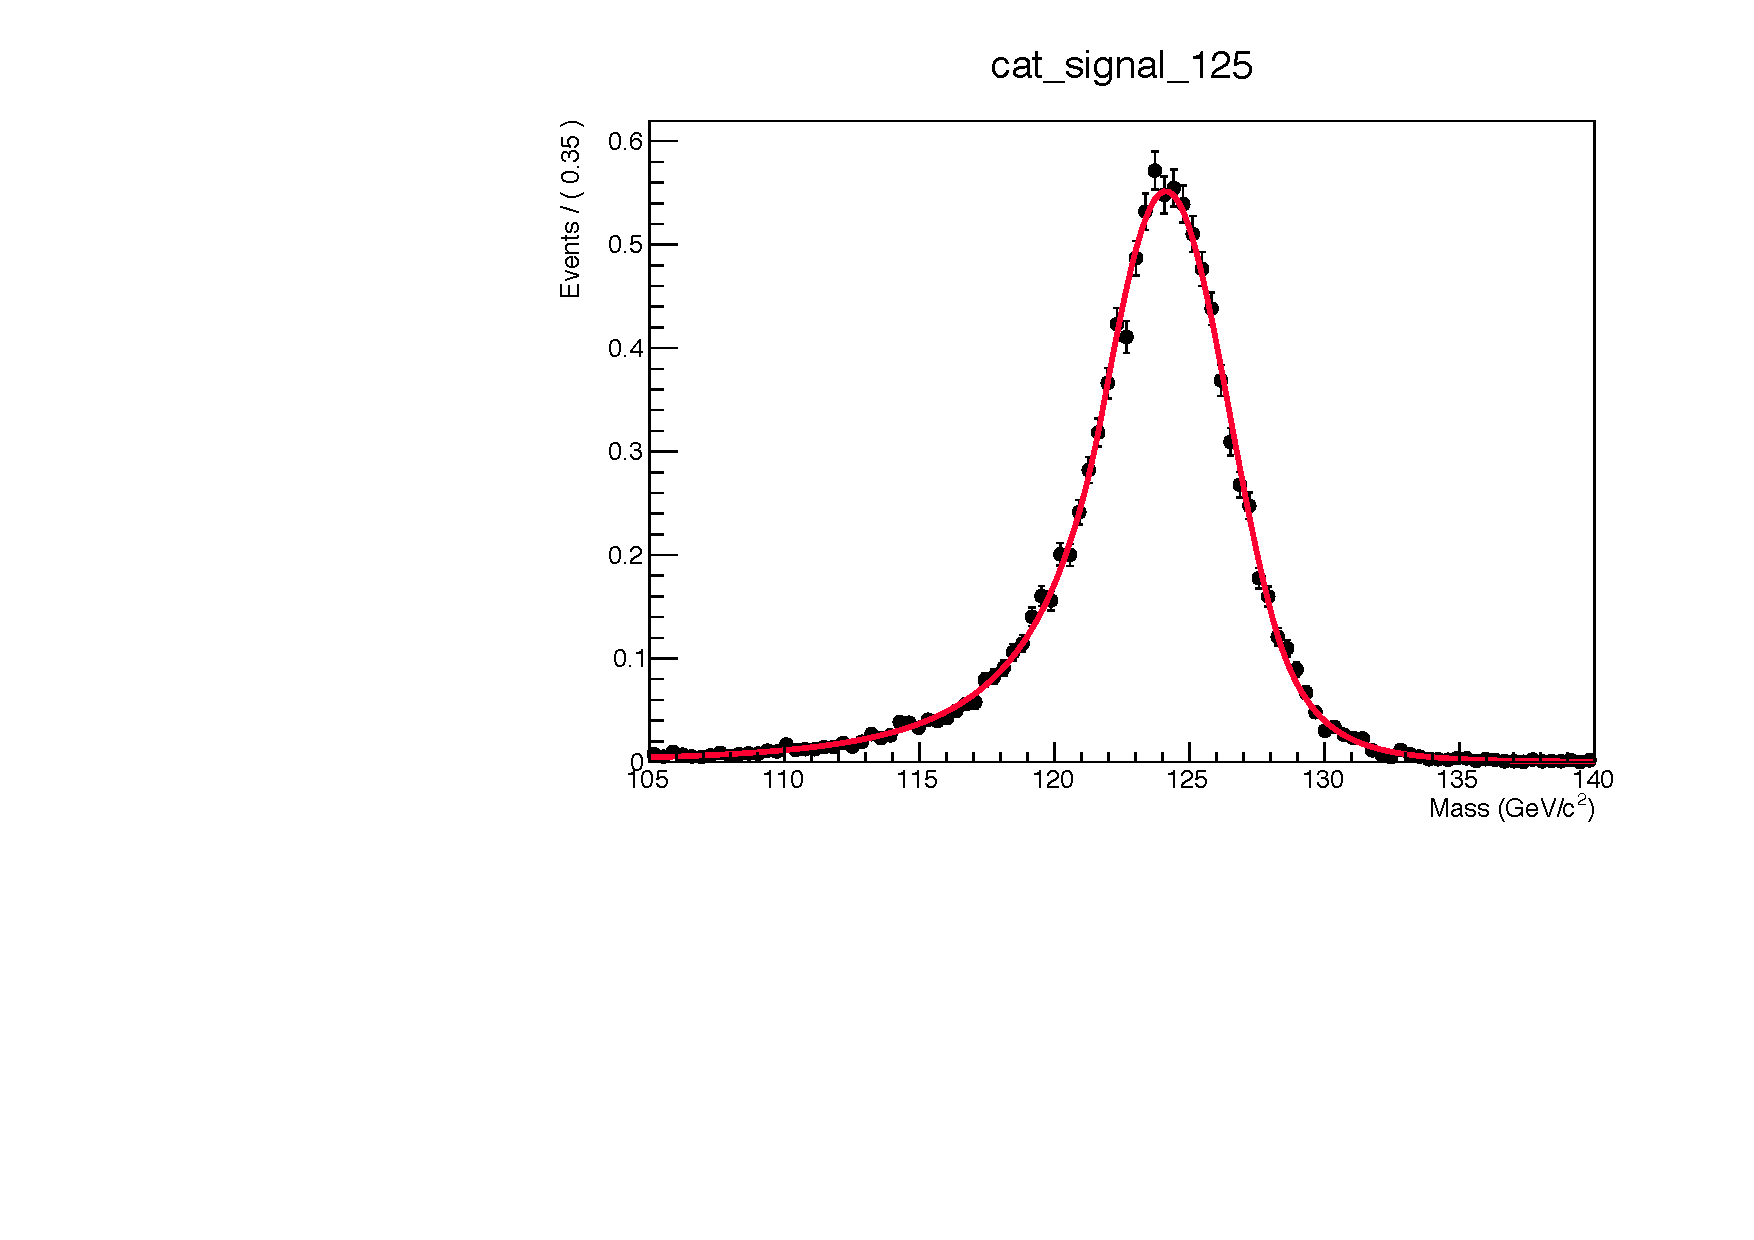
\includegraphics[width=0.3\textwidth]{Figures/SignalModelling/Signal_Parametrization/2017/ggH_4e_2017_125_Sim.pdf}
%		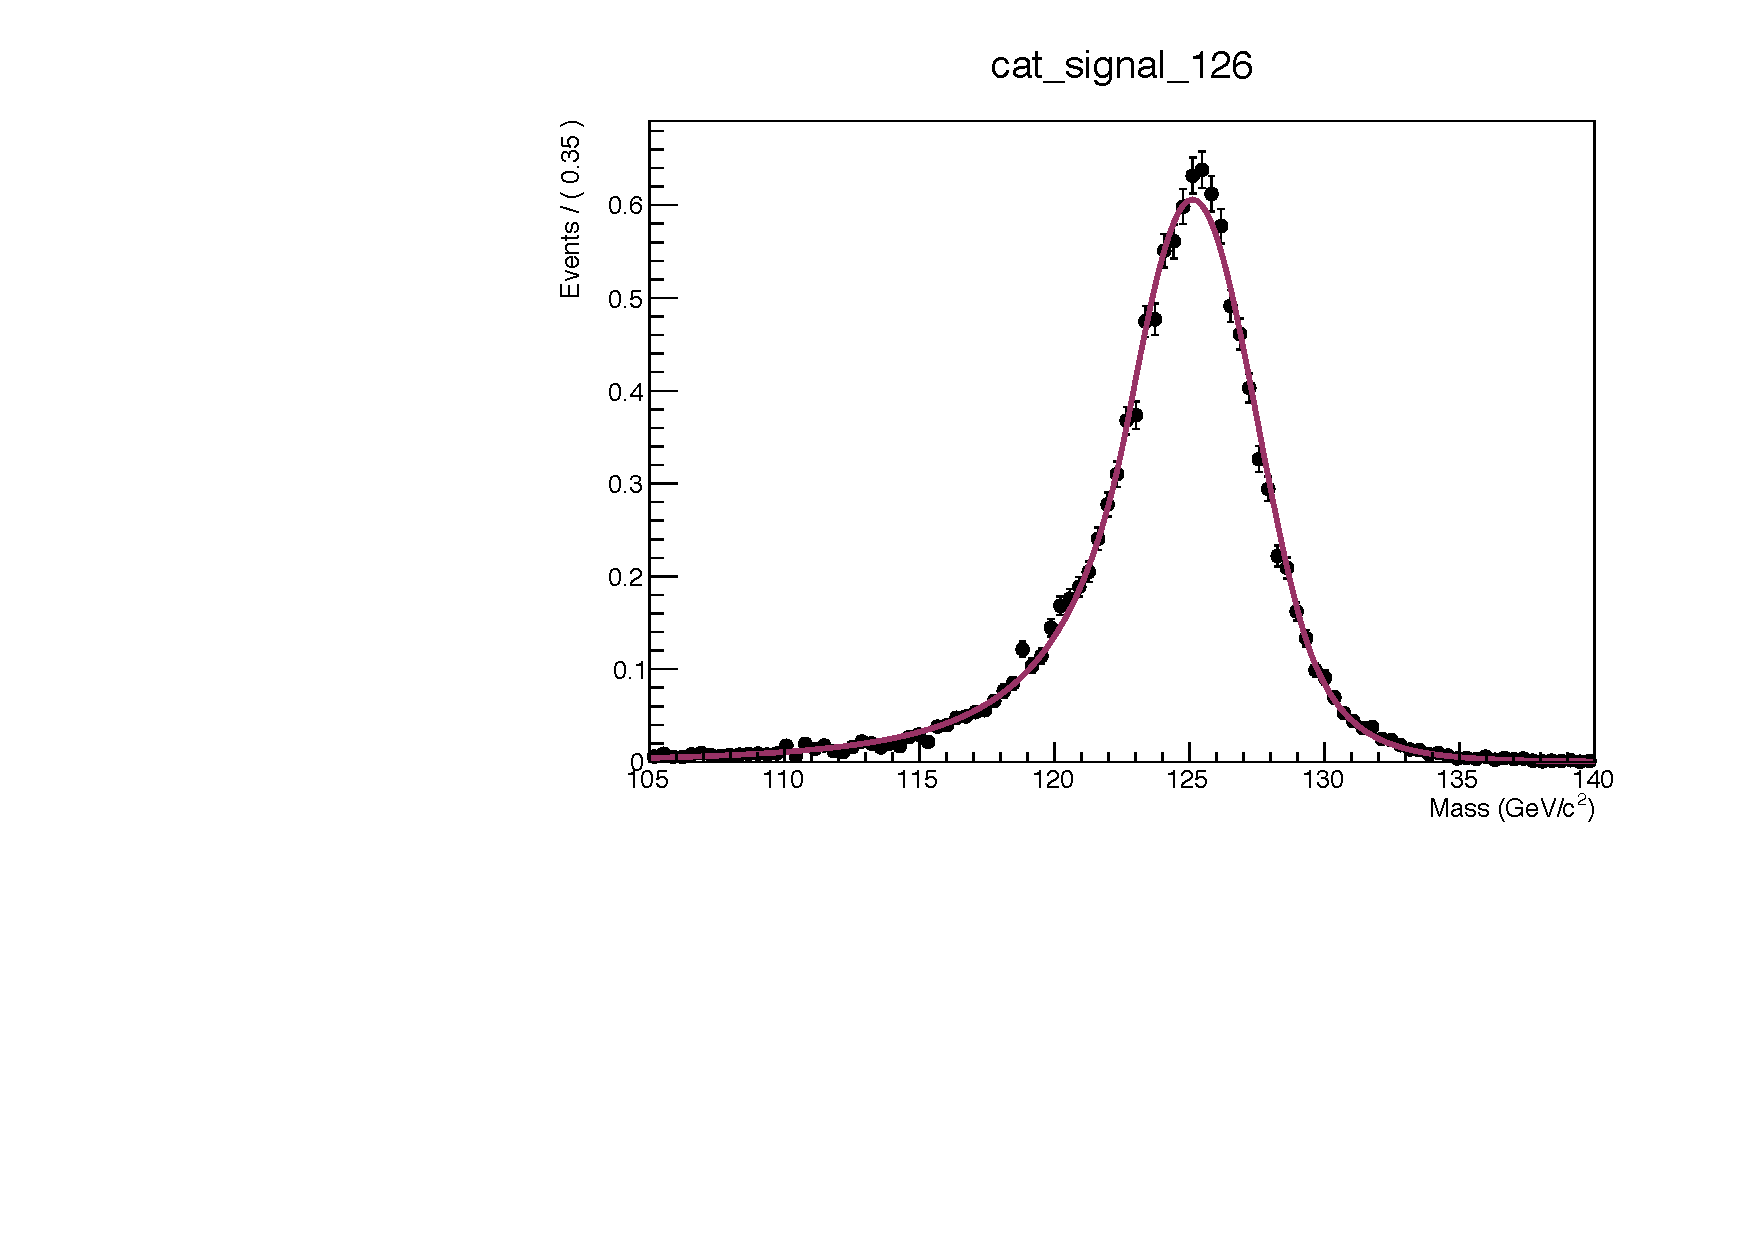
\includegraphics[width=0.3\textwidth]{Figures/SignalModelling/Signal_Parametrization/2017/ggH_4e_2017_126_Sim.pdf} 
%		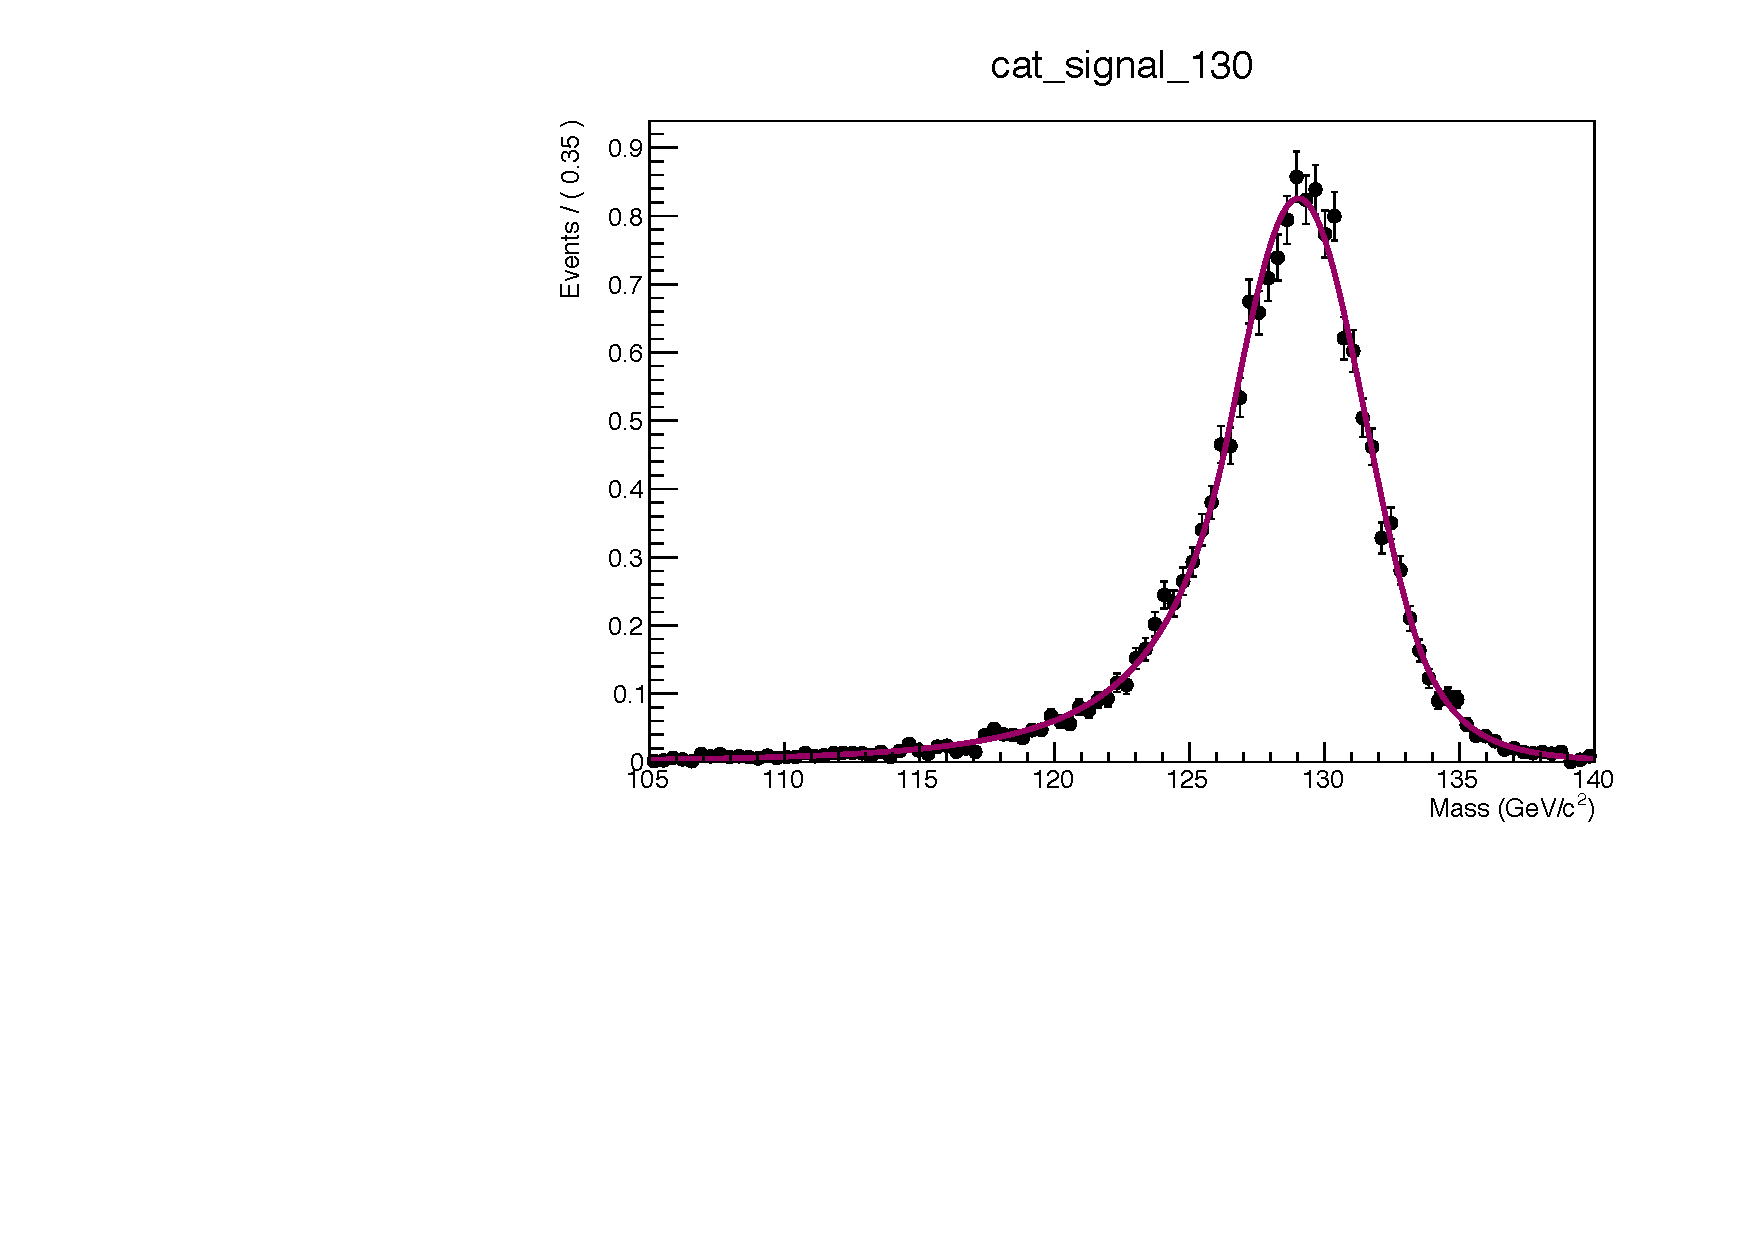
\includegraphics[width=0.3\textwidth]{Figures/SignalModelling/Signal_Parametrization/2017/ggH_4e_2017_130_Sim.pdf}
%		\caption{Simultaneous fit for ggH production mode, in 2017, for different mass points, 
%		in 4e final state.}
%	\label{signal_lineshape_2017_full_1}
%	\end{center}
%\end{figure}
%\begin{figure}[!htbp]
%	\begin{center}
%		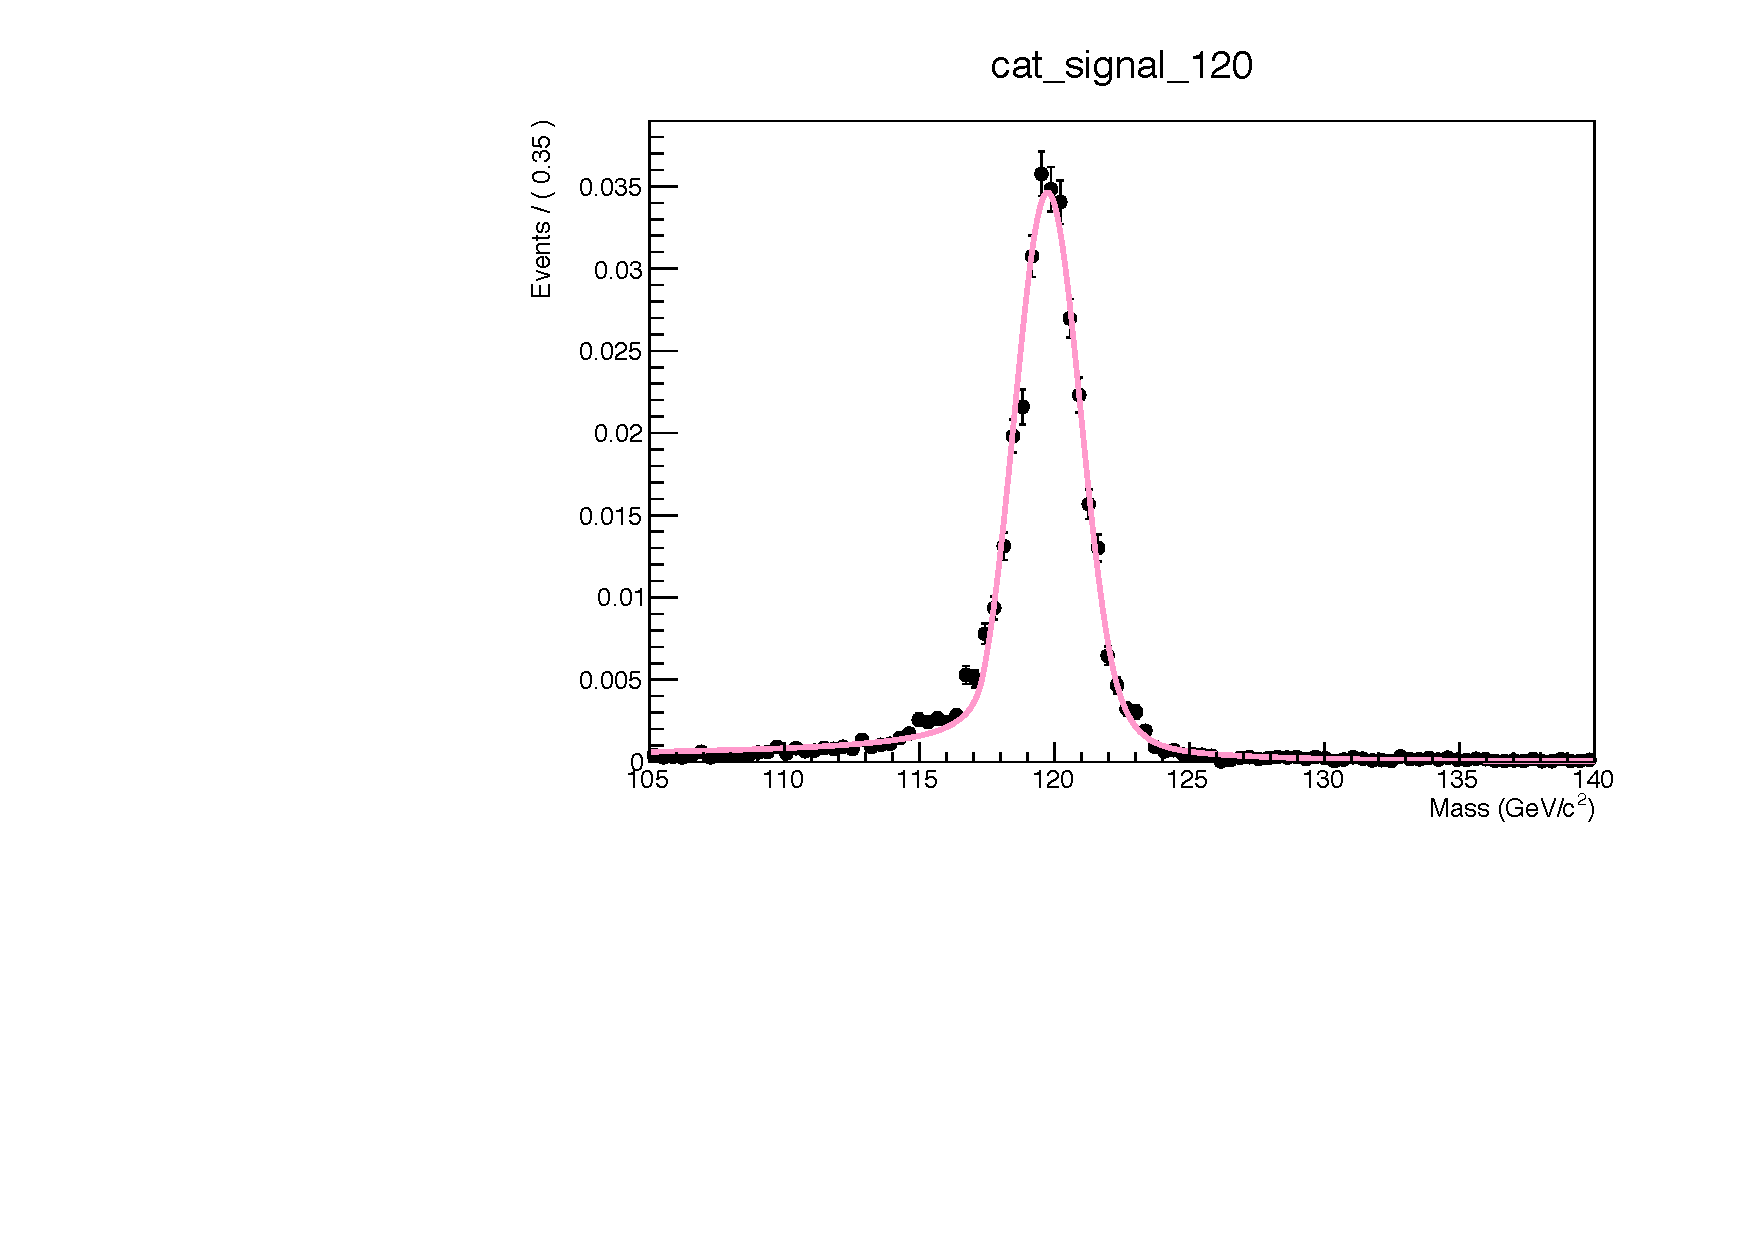
\includegraphics[width=0.3\textwidth]{Figures/SignalModelling/Signal_Parametrization/2017/WH_4mu_2017_120_Sim.pdf}
%		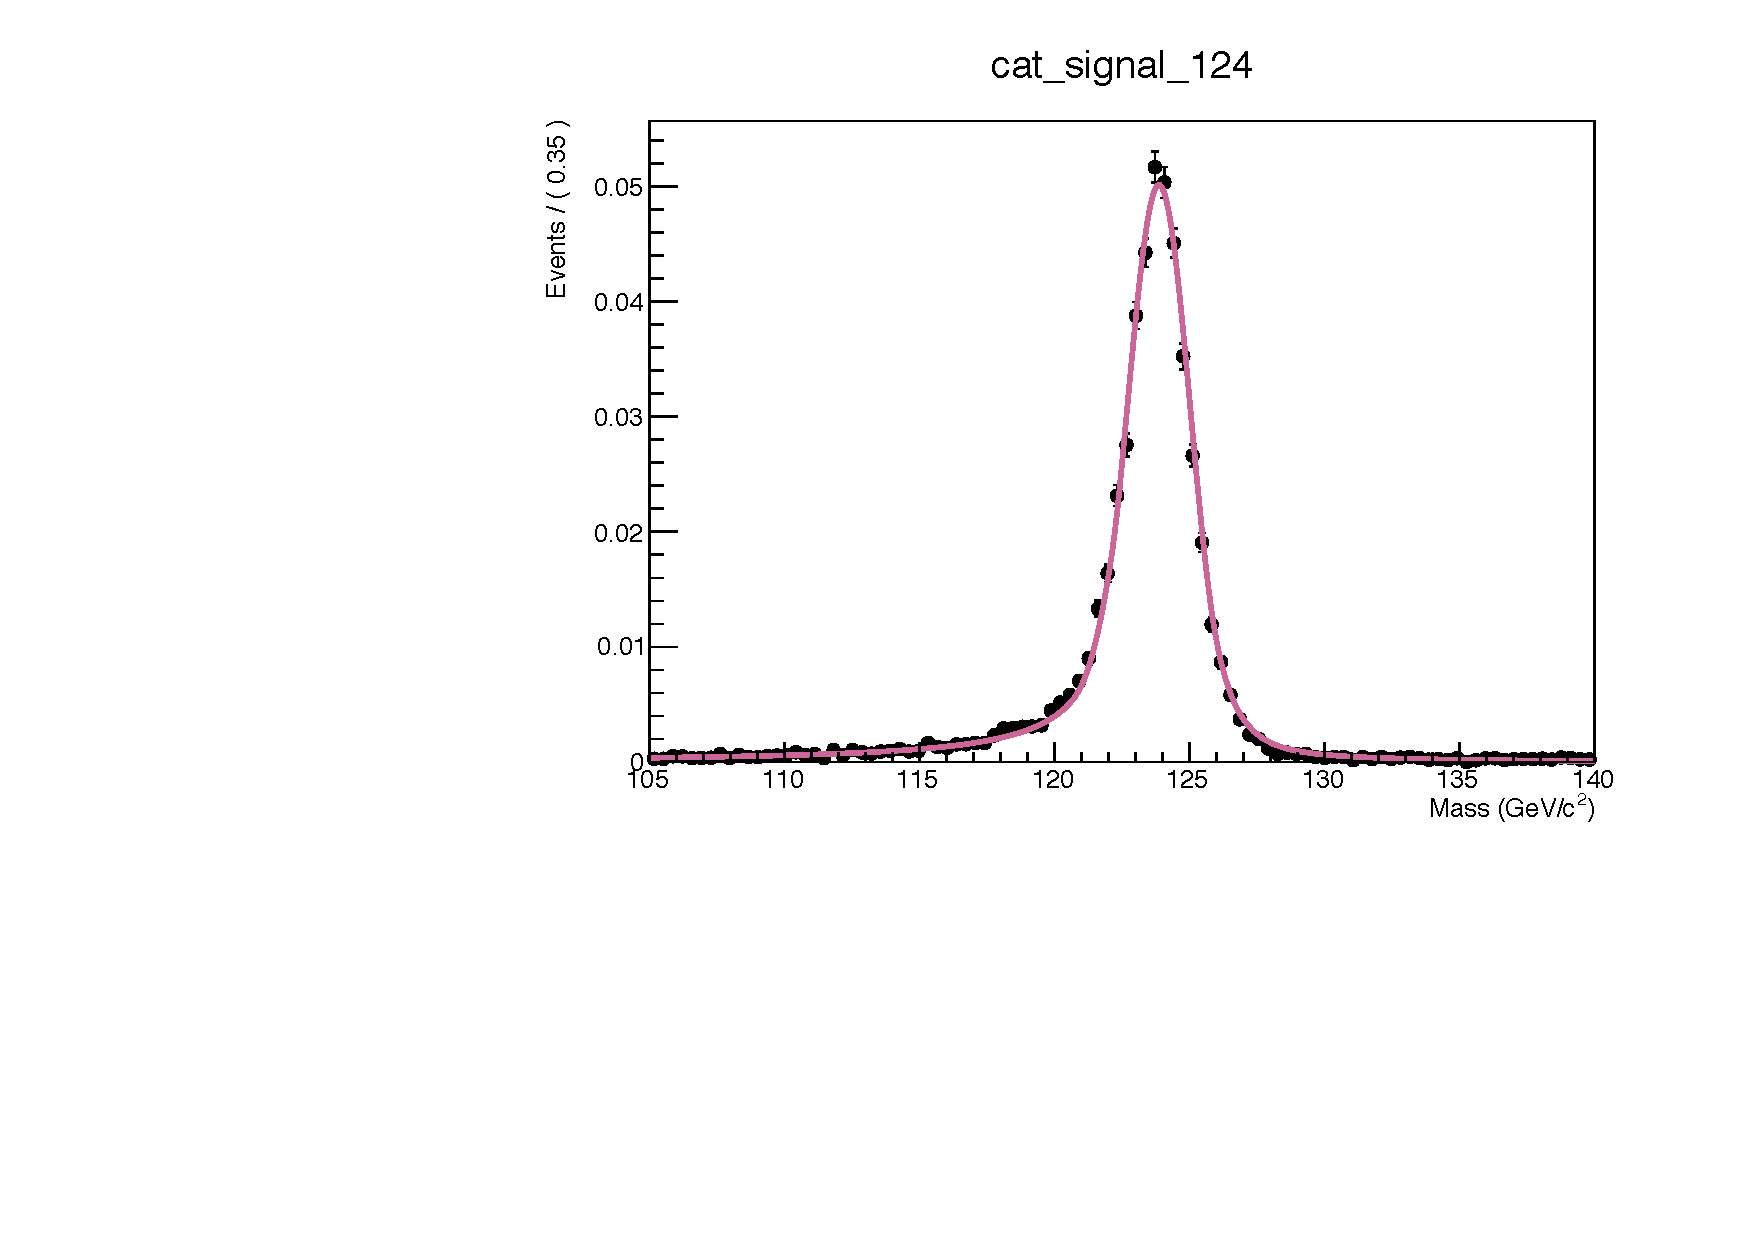
\includegraphics[width=0.3\textwidth]{Figures/SignalModelling/Signal_Parametrization/2017/WH_4mu_2017_124_Sim.pdf}
%   		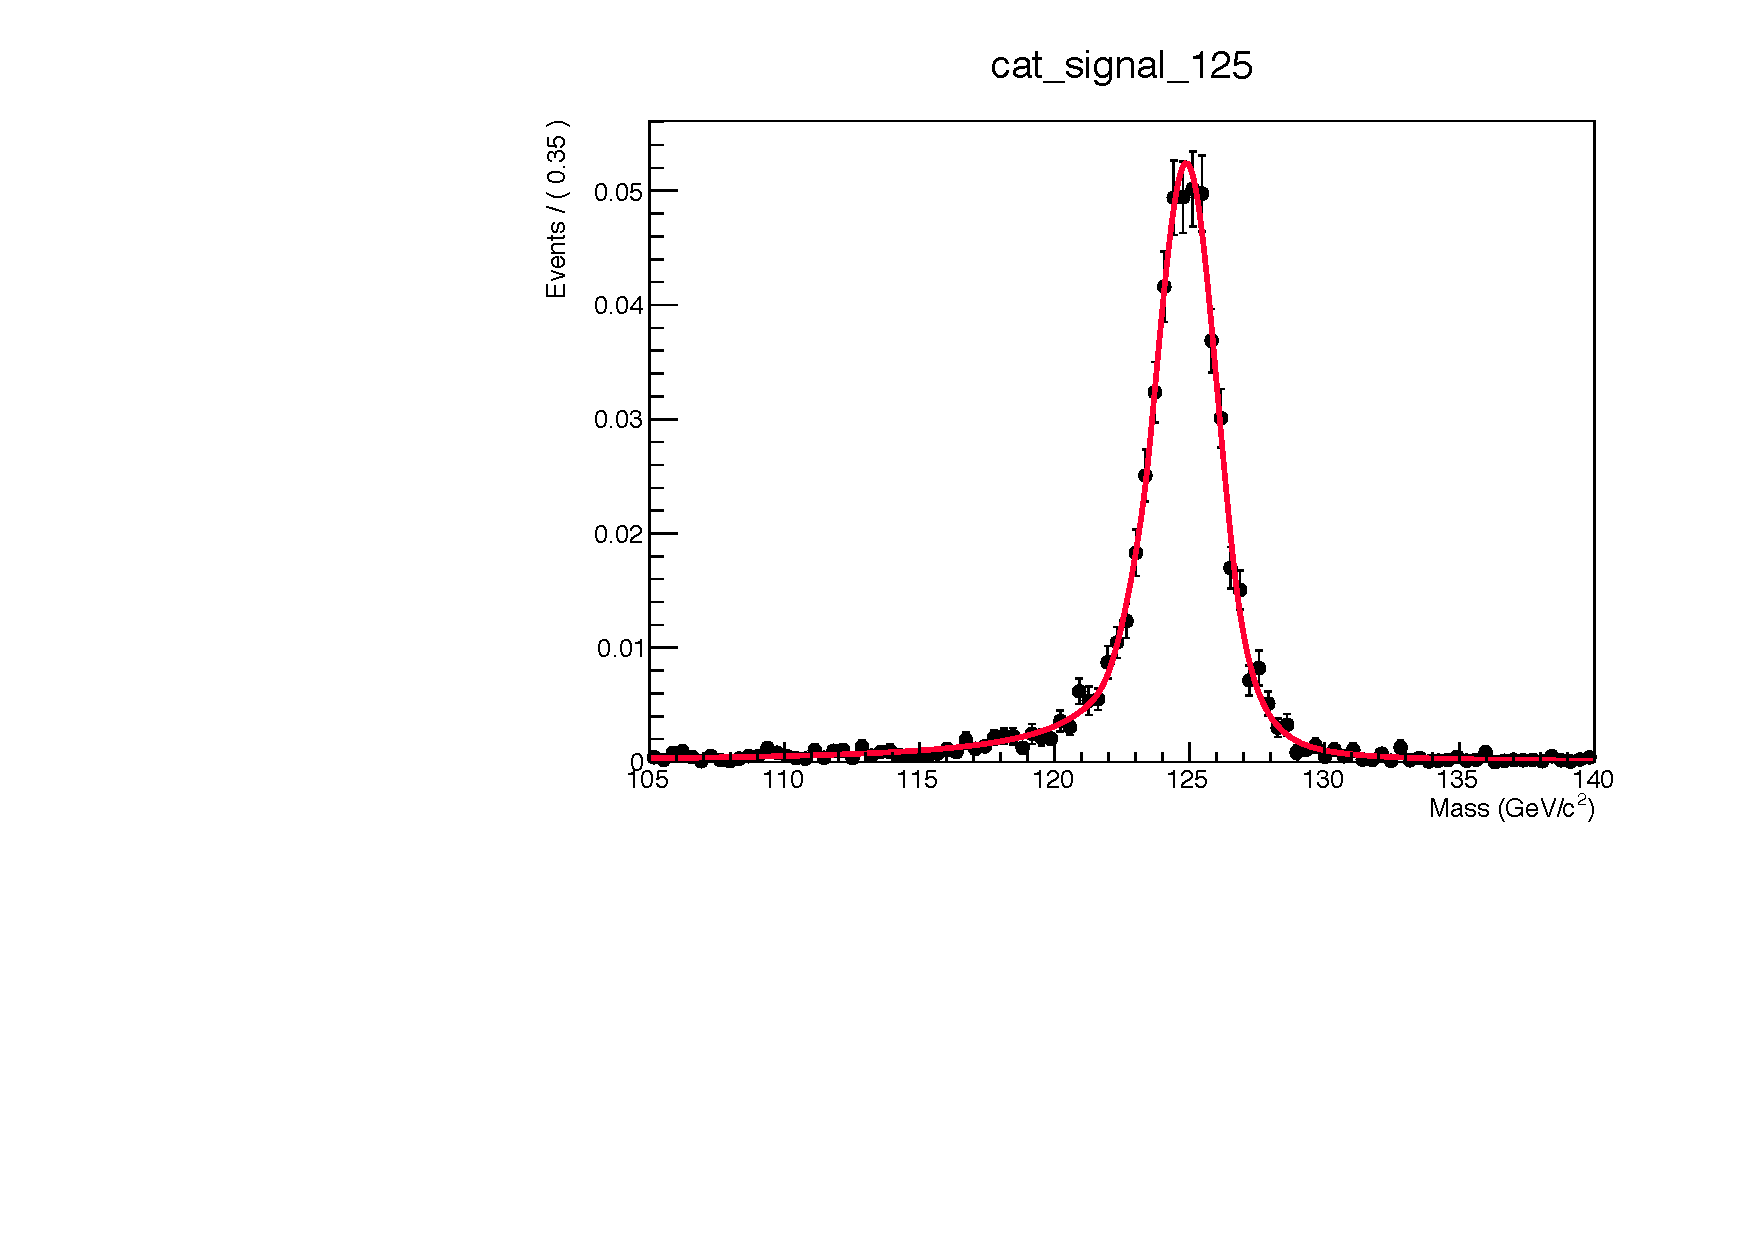
\includegraphics[width=0.3\textwidth]{Figures/SignalModelling/Signal_Parametrization/2017/WH_4mu_2017_125_Sim.pdf}
%		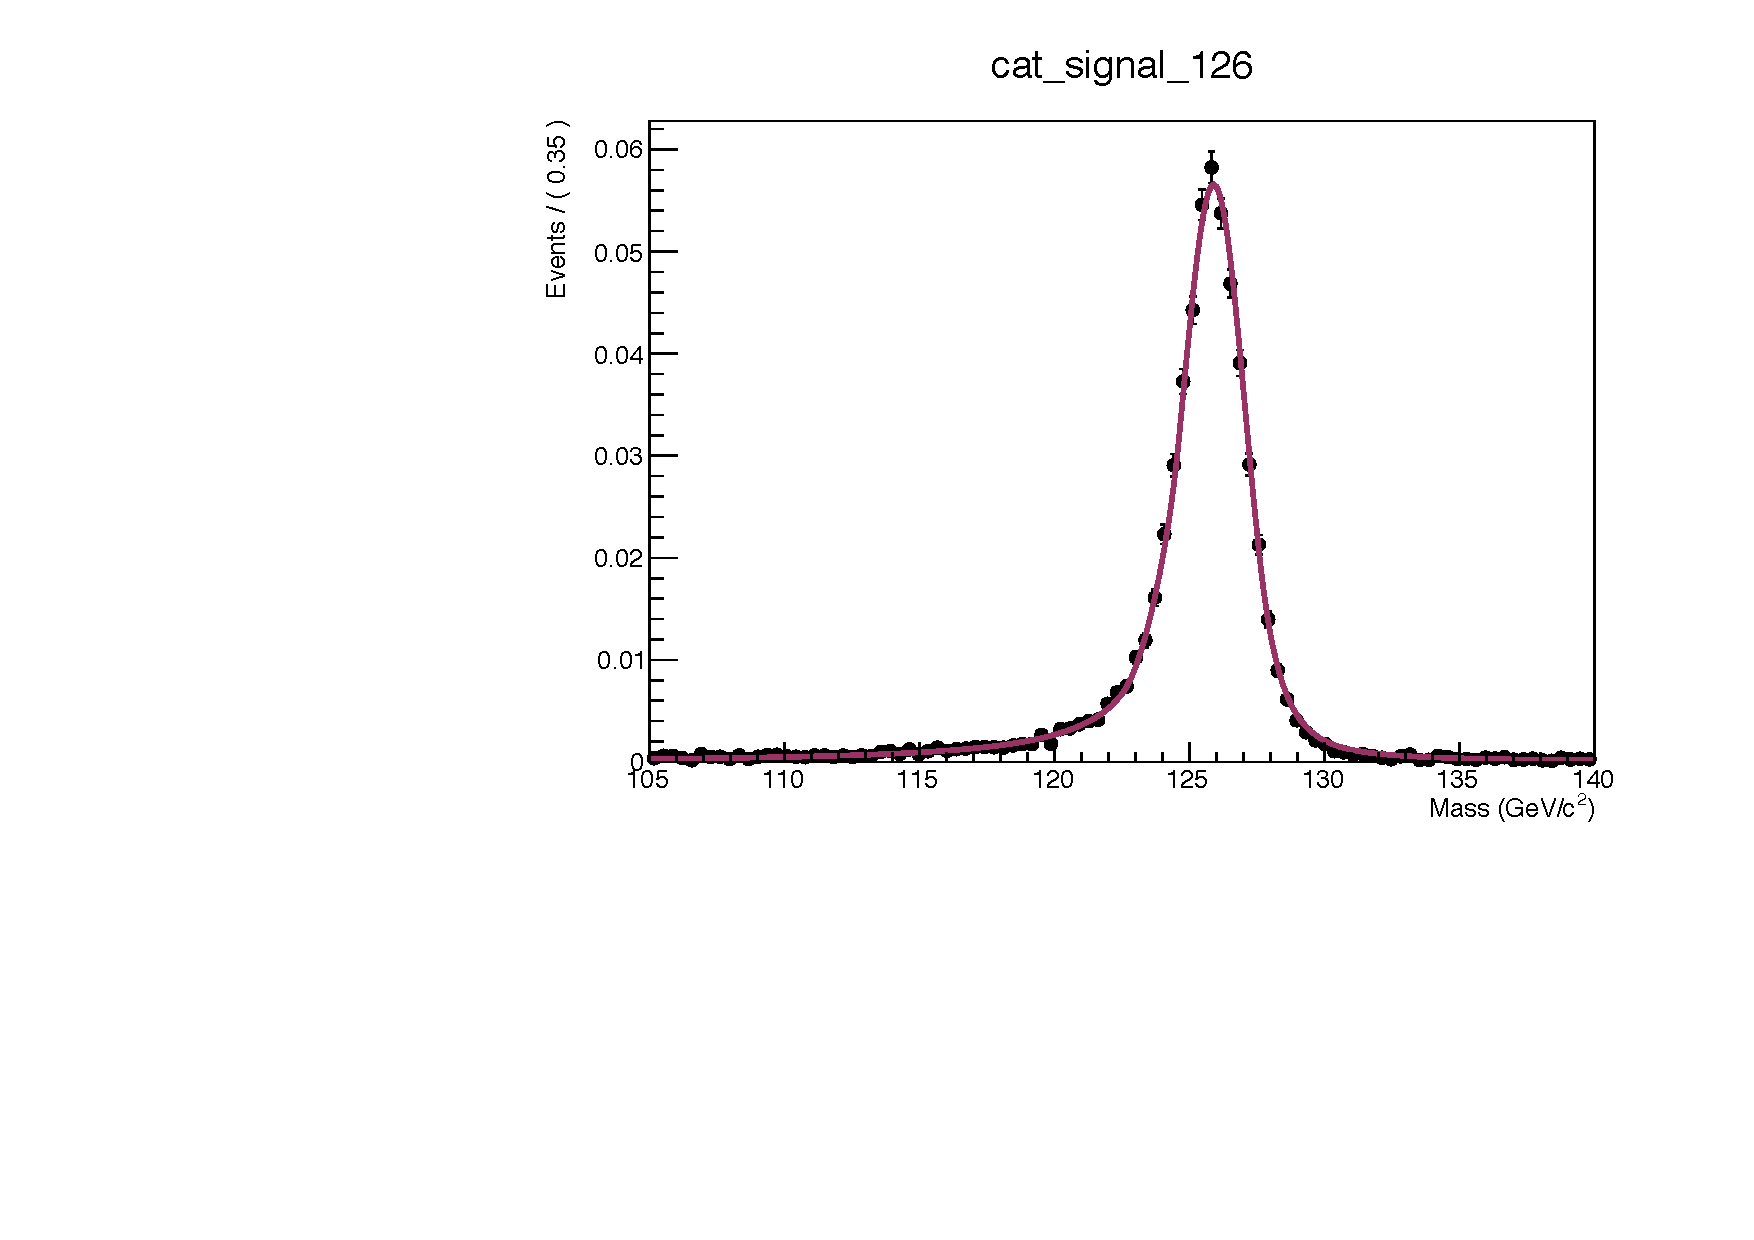
\includegraphics[width=0.3\textwidth]{Figures/SignalModelling/Signal_Parametrization/2017/WH_4mu_2017_126_Sim.pdf} 
%		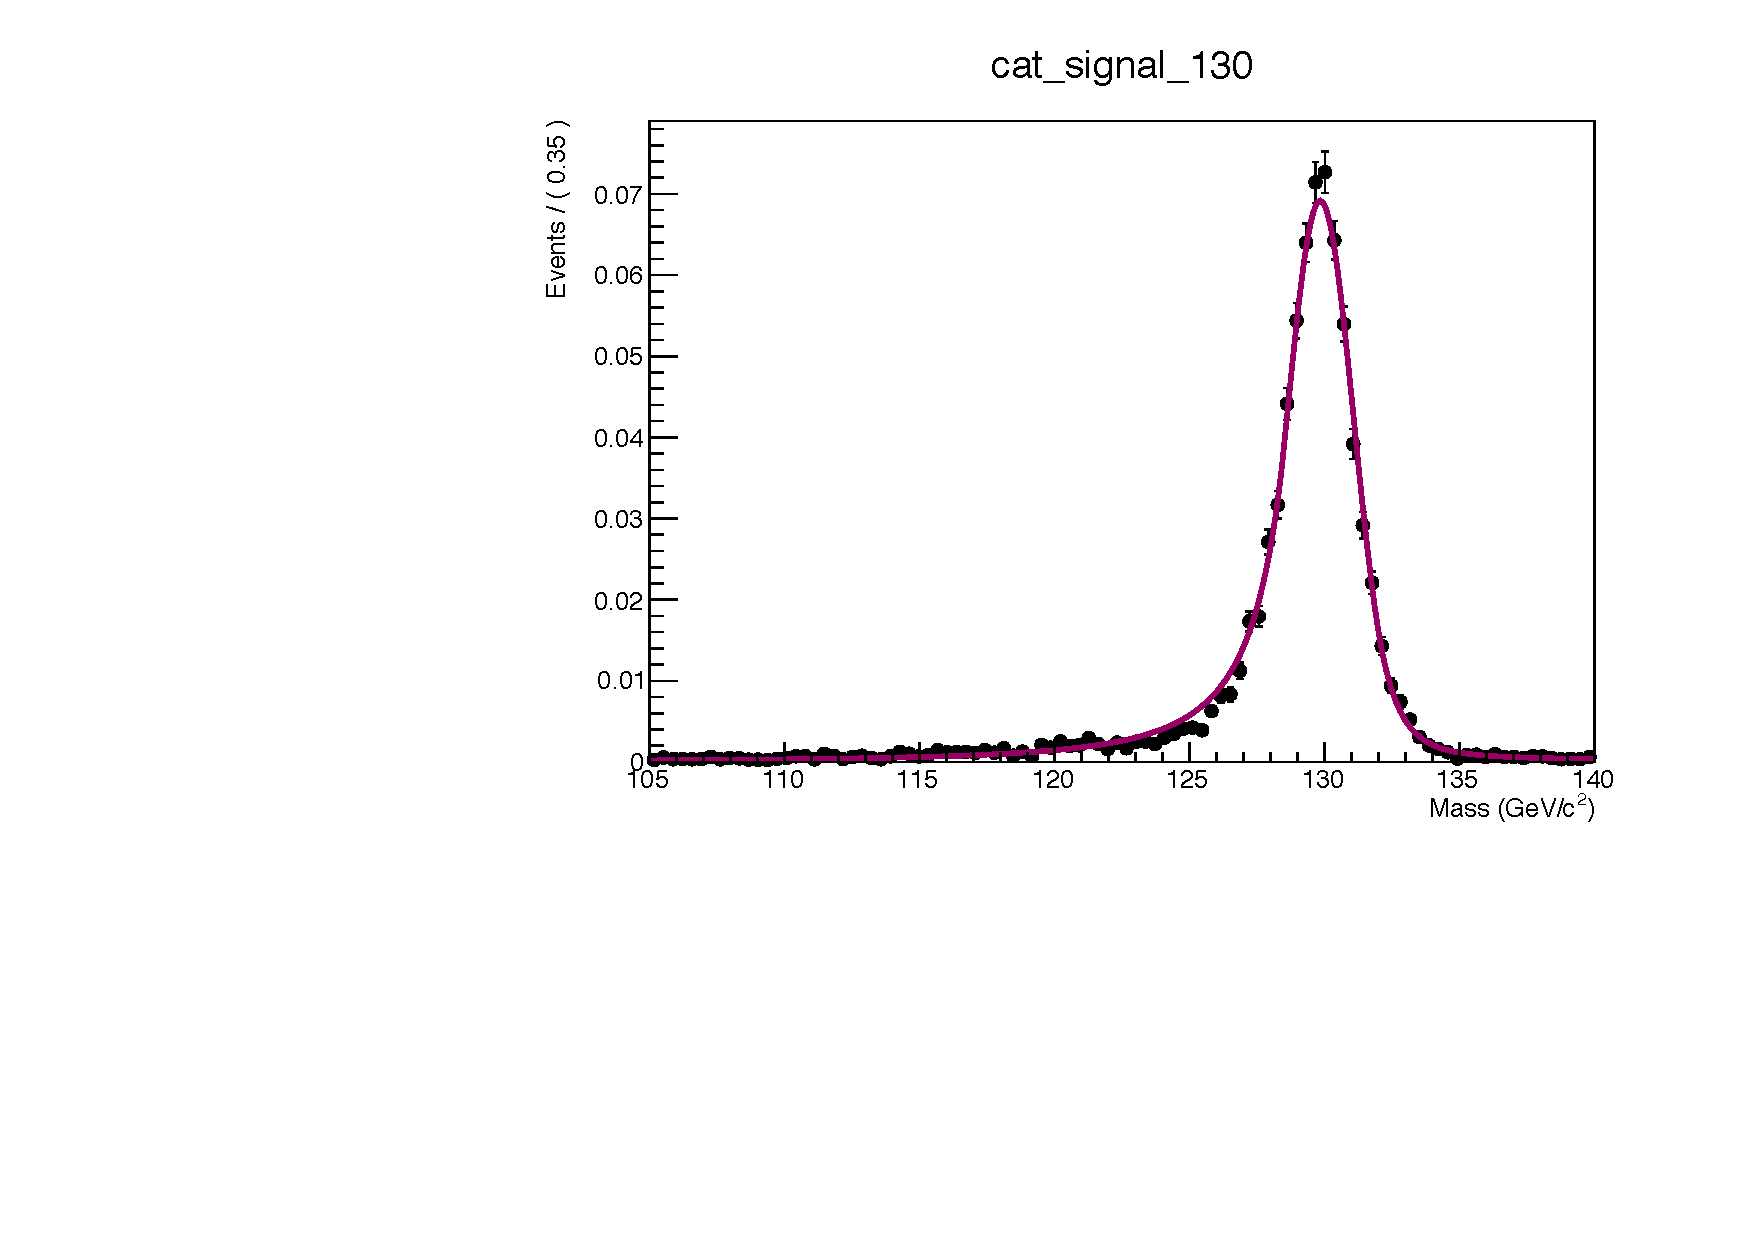
\includegraphics[width=0.3\textwidth]{Figures/SignalModelling/Signal_Parametrization/2017/WH_4mu_2017_130_Sim.pdf}
%		\caption{Simultaneous fit for WH production mode, in 2017, for different mass points, 
%		in 4$\mu$ final state.}
%	\label{signal_lineshape_2017_full_2}
%	\end{center}
%\end{figure}
%\begin{figure}[!htbp]
%	\begin{center}
%		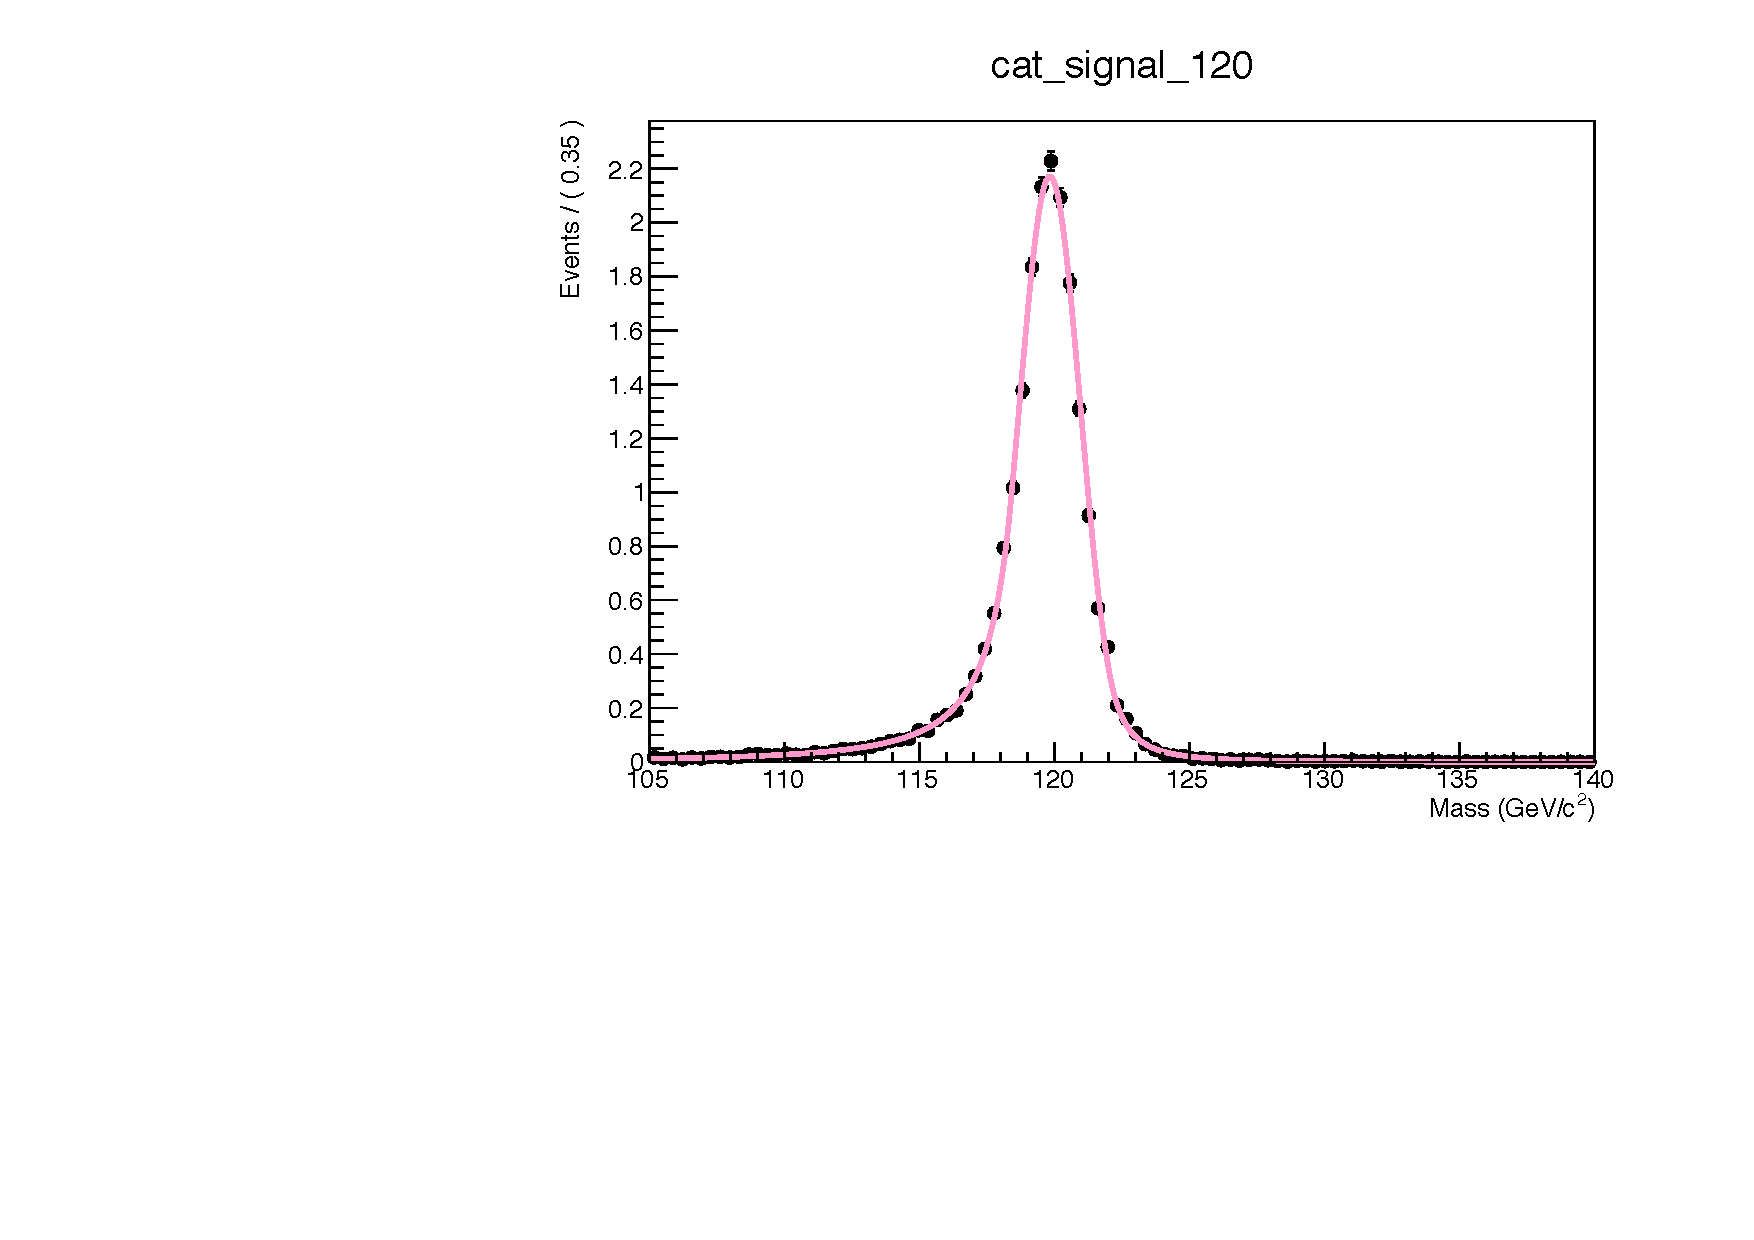
\includegraphics[width=0.3\textwidth]{Figures/SignalModelling/Signal_Parametrization/2018/ggH_4mu_2018_120_Sim.pdf}
%		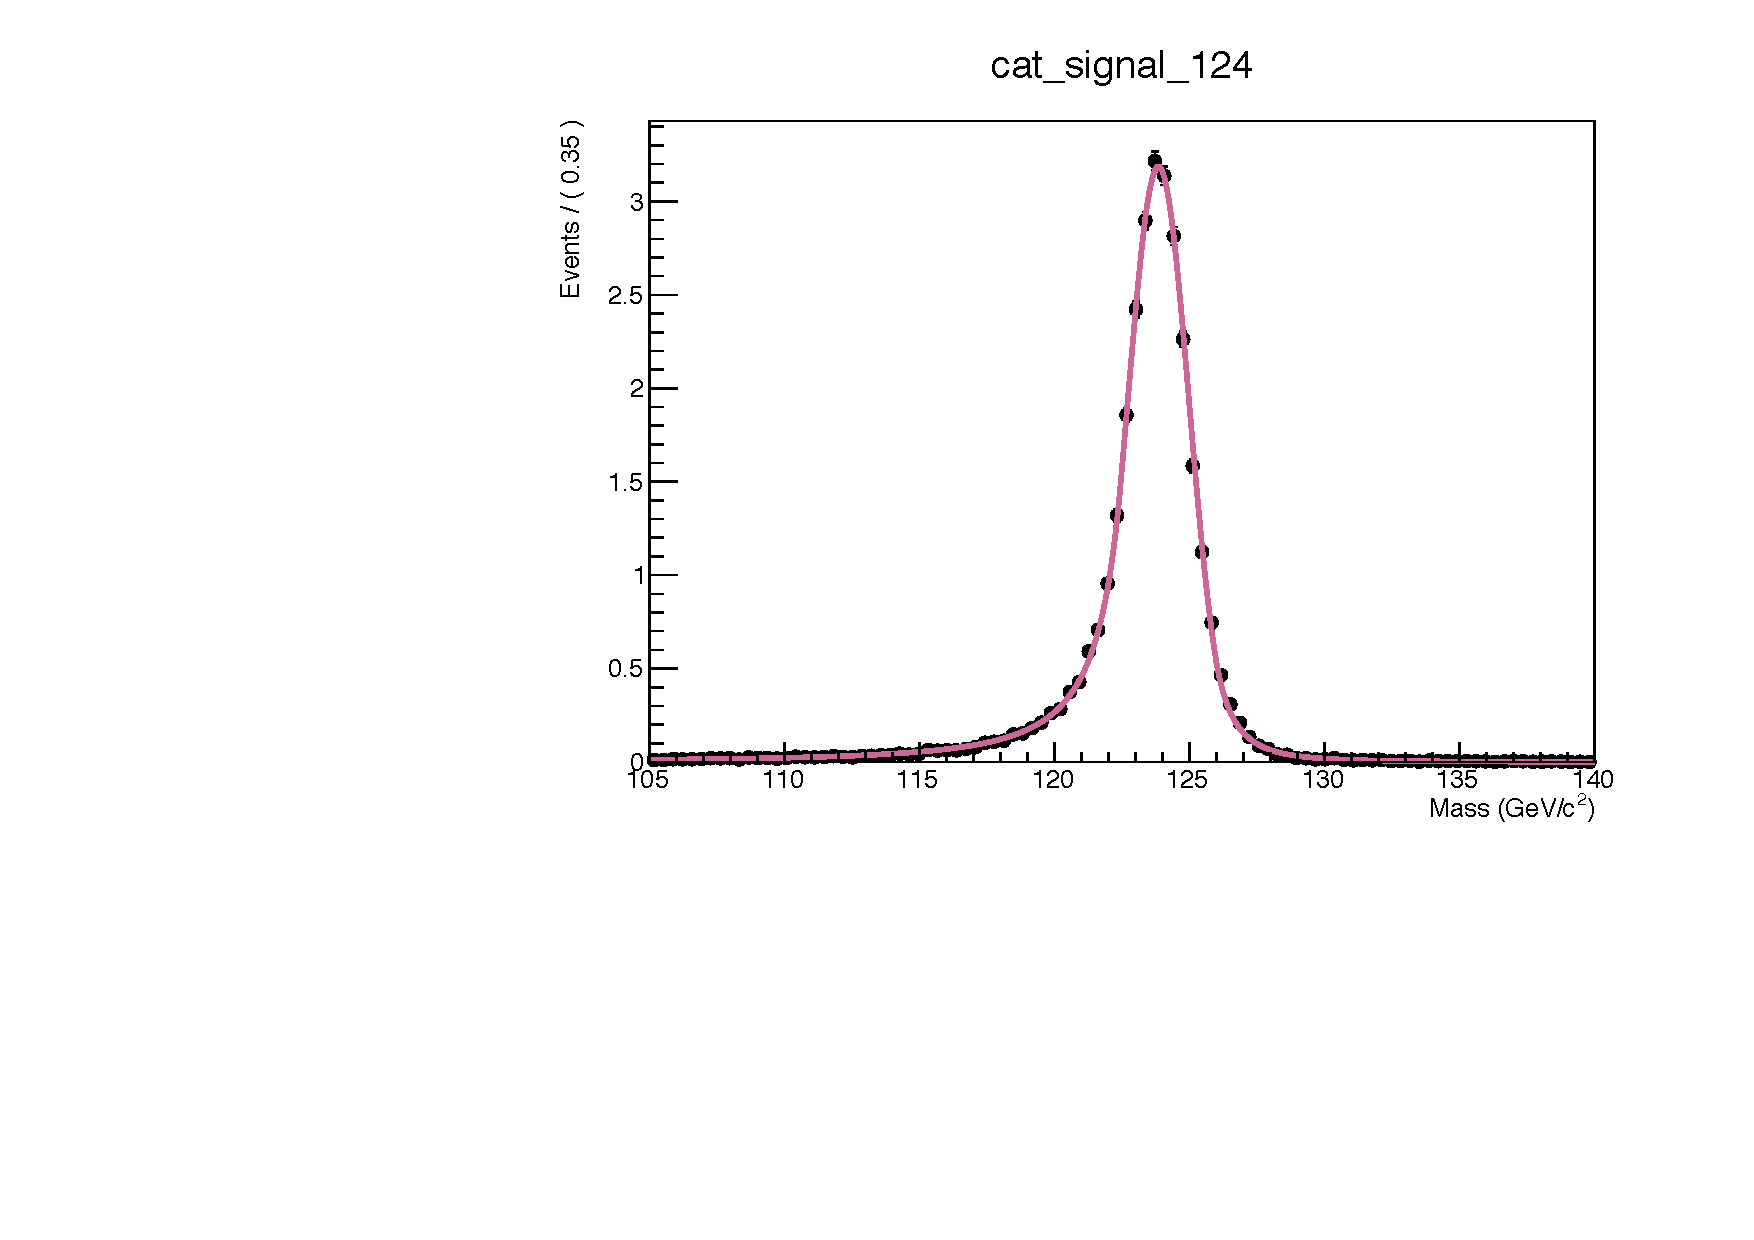
\includegraphics[width=0.3\textwidth]{Figures/SignalModelling/Signal_Parametrization/2018/ggH_4mu_2018_124_Sim.pdf}
%   		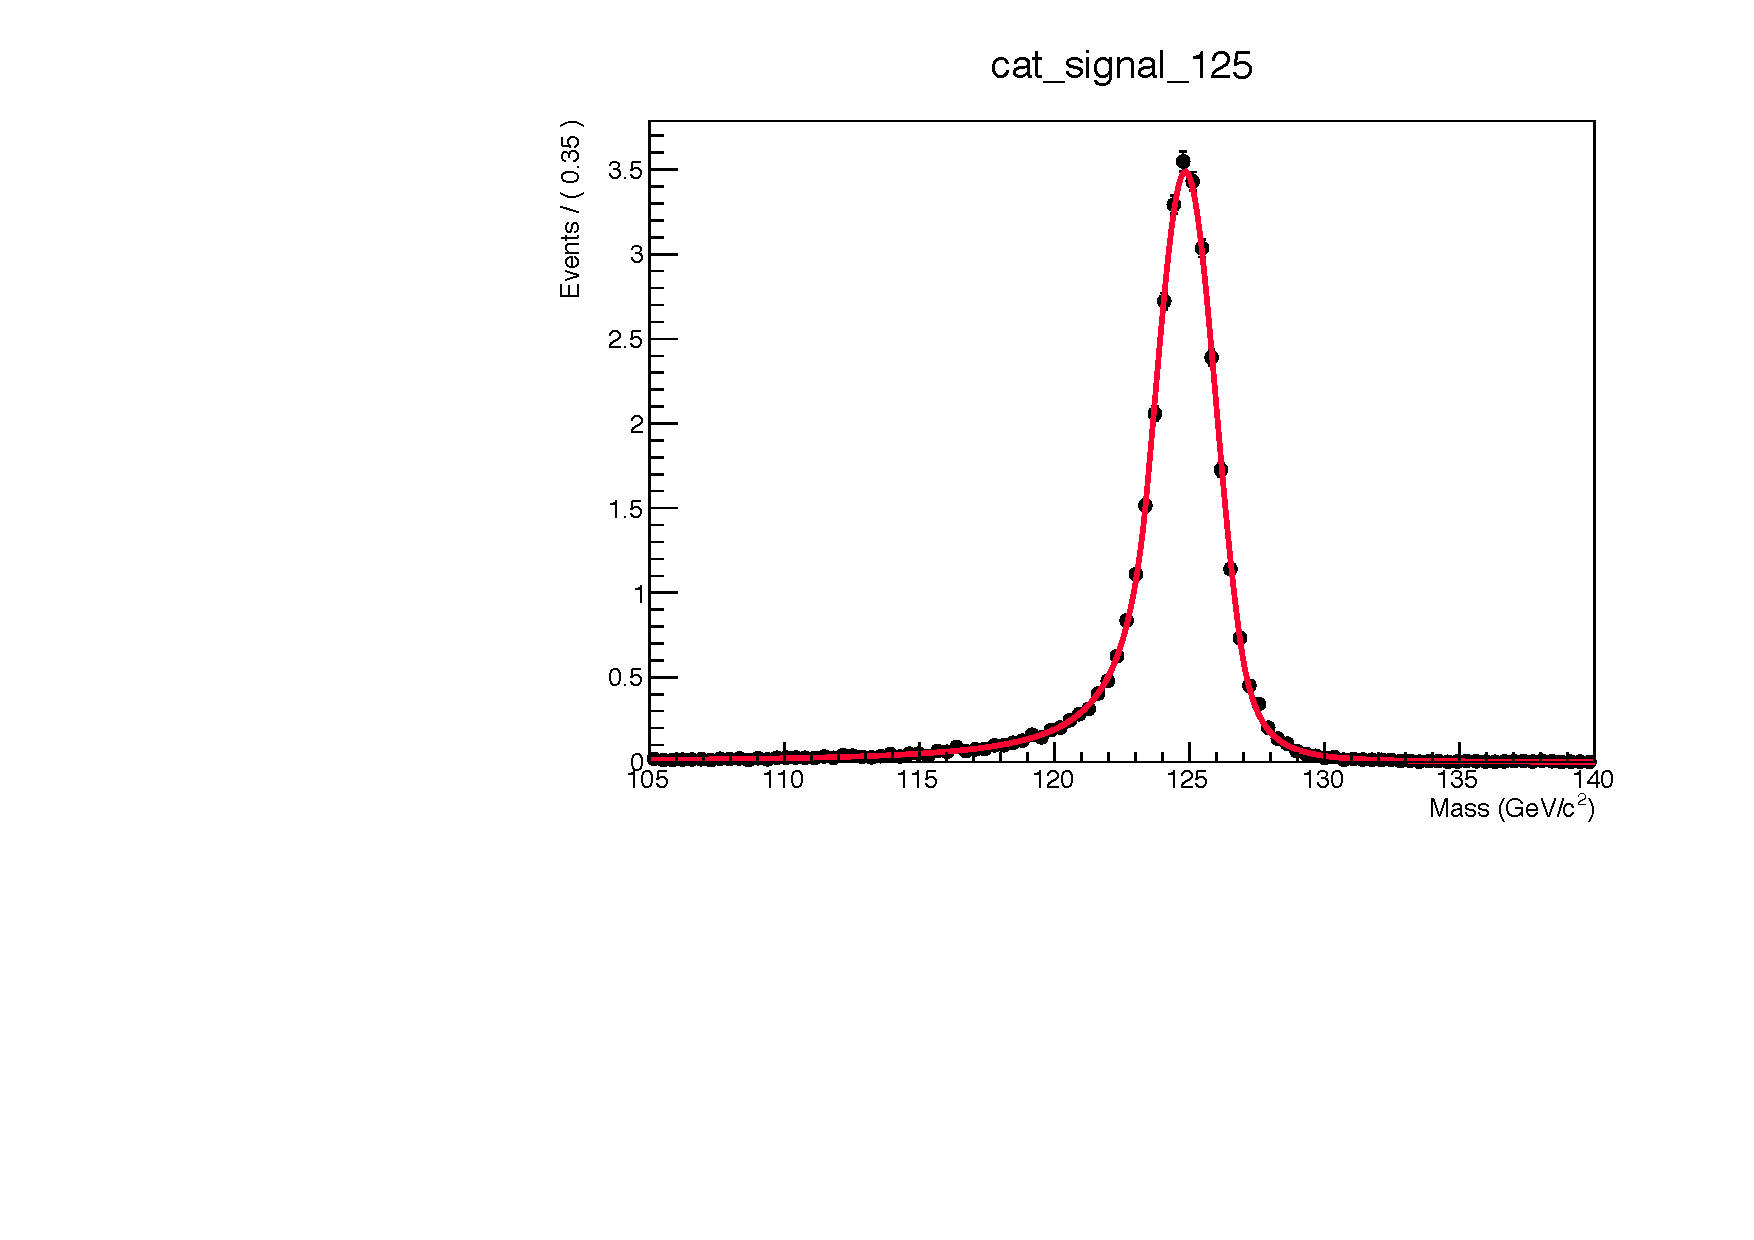
\includegraphics[width=0.3\textwidth]{Figures/SignalModelling/Signal_Parametrization/2018/ggH_4mu_2018_125_Sim.pdf}
%		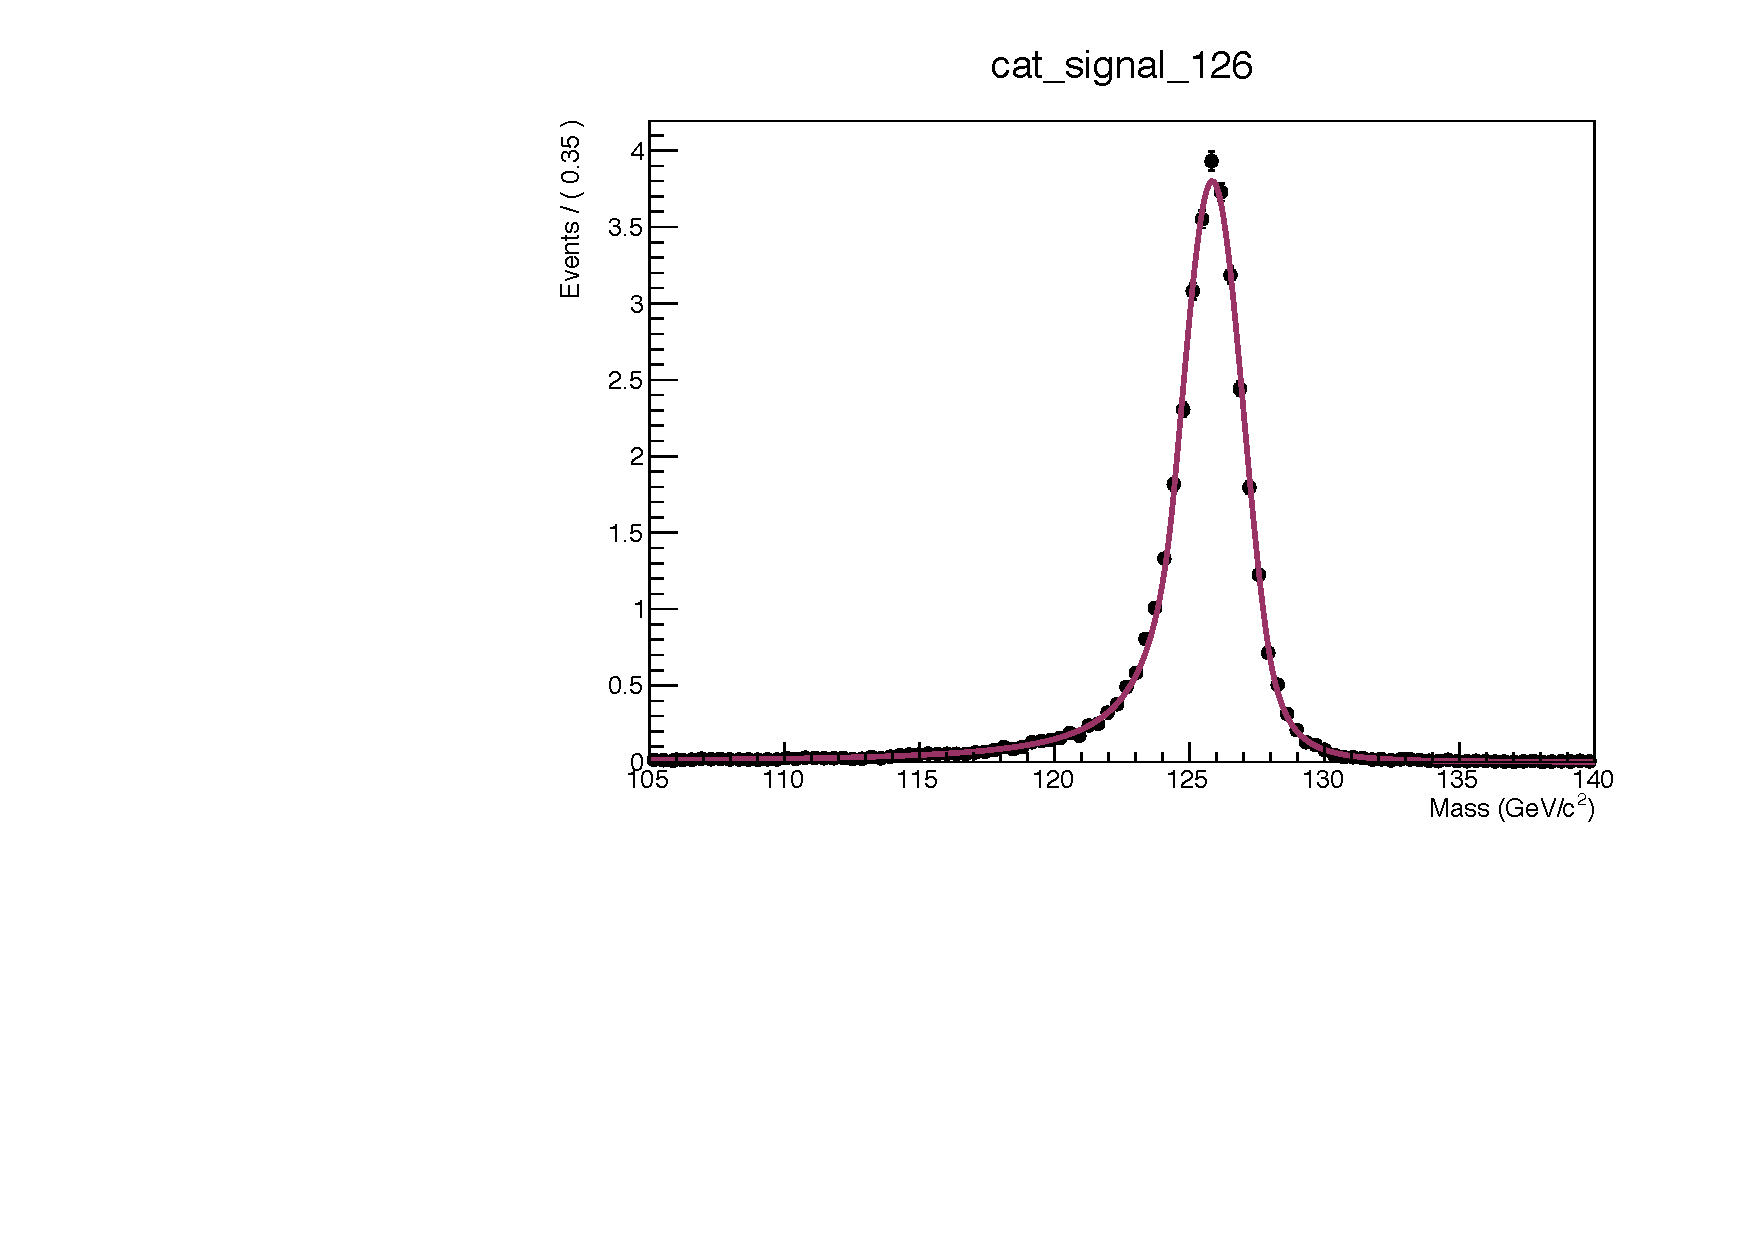
\includegraphics[width=0.3\textwidth]{Figures/SignalModelling/Signal_Parametrization/2018/ggH_4mu_2018_126_Sim.pdf} 
%		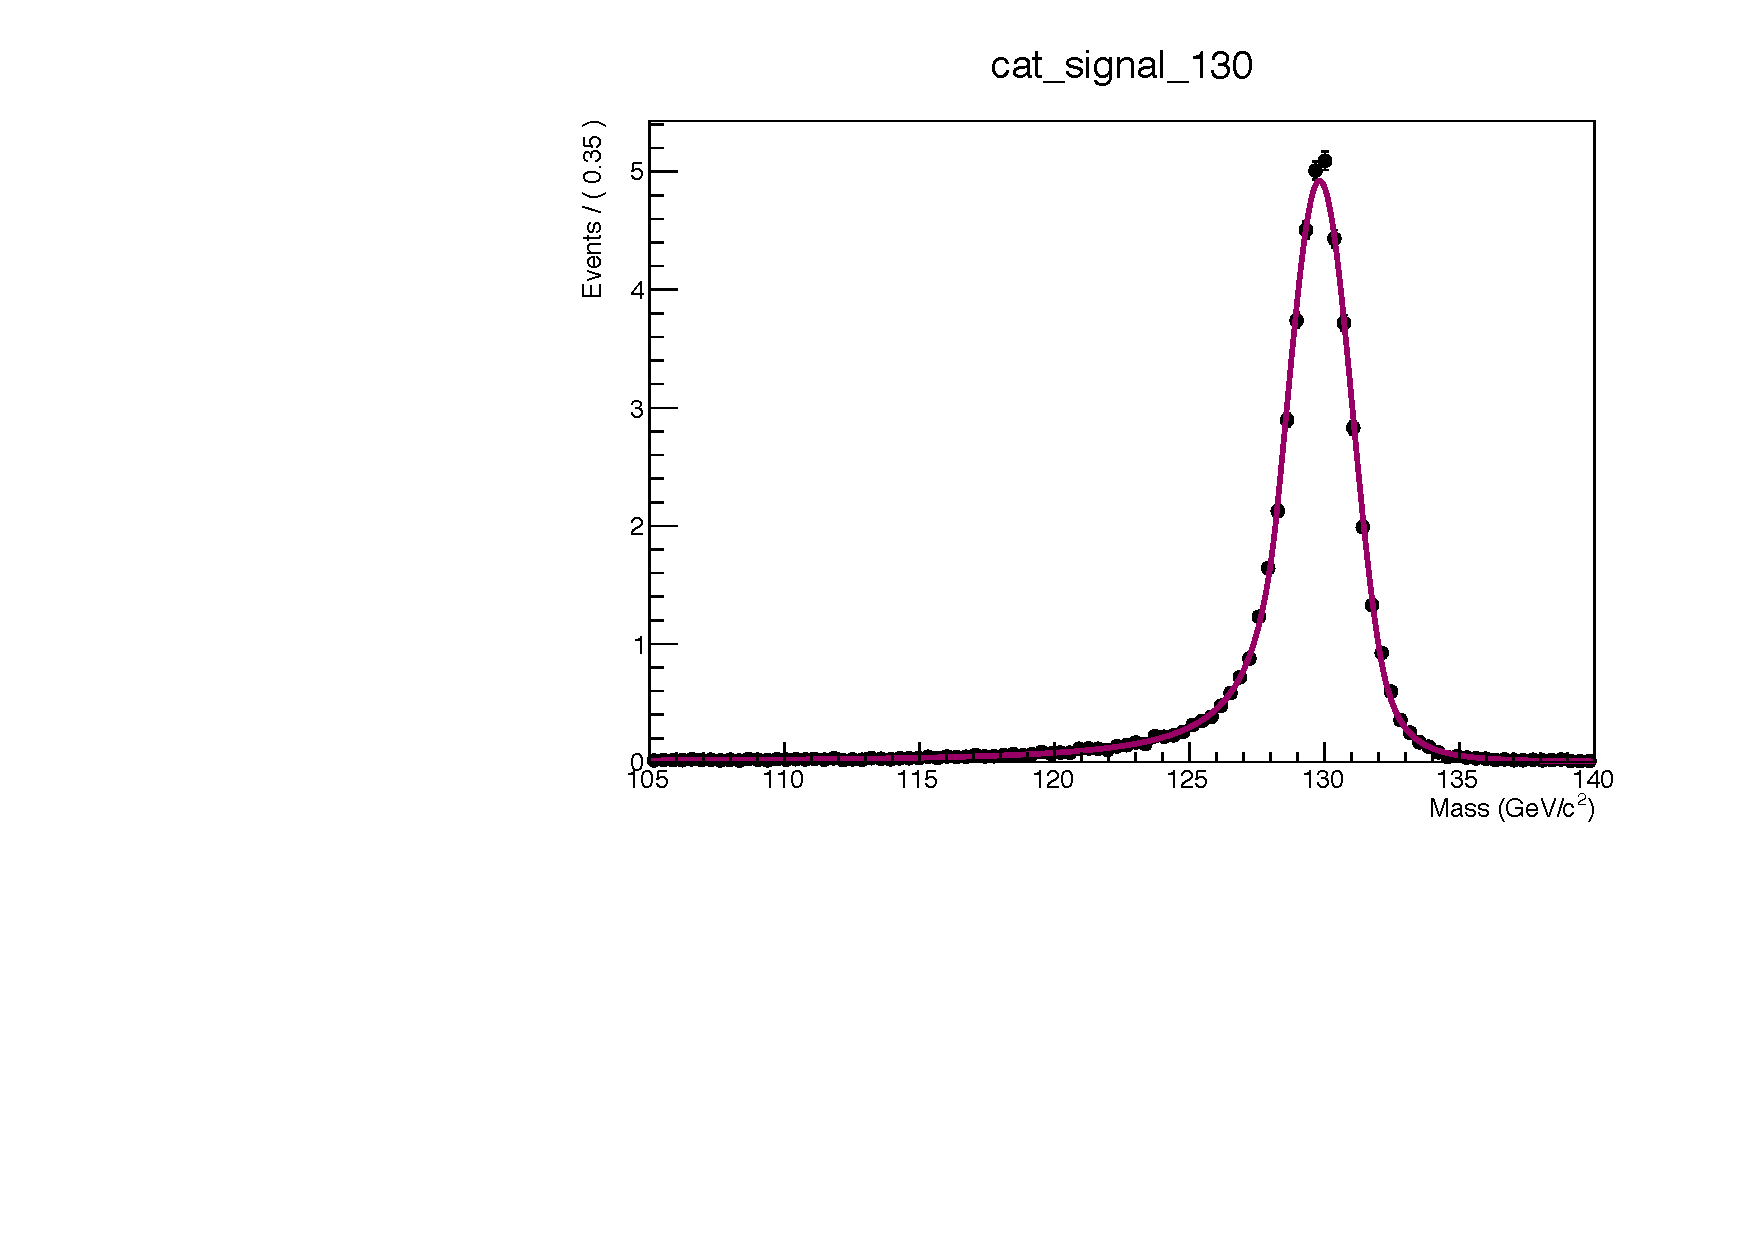
\includegraphics[width=0.3\textwidth]{Figures/SignalModelling/Signal_Parametrization/2018/ggH_4mu_2018_130_Sim.pdf}
%		\caption{Simultaneous fit for ggH production mode, in 2018, for different mass points, 
%		in 4$\mu$ final state.}
%	\label{signal_lineshape_2018_full_1}
%	\end{center}
%\end{figure}
%\begin{figure}[!htbp]
%	\begin{center}
%		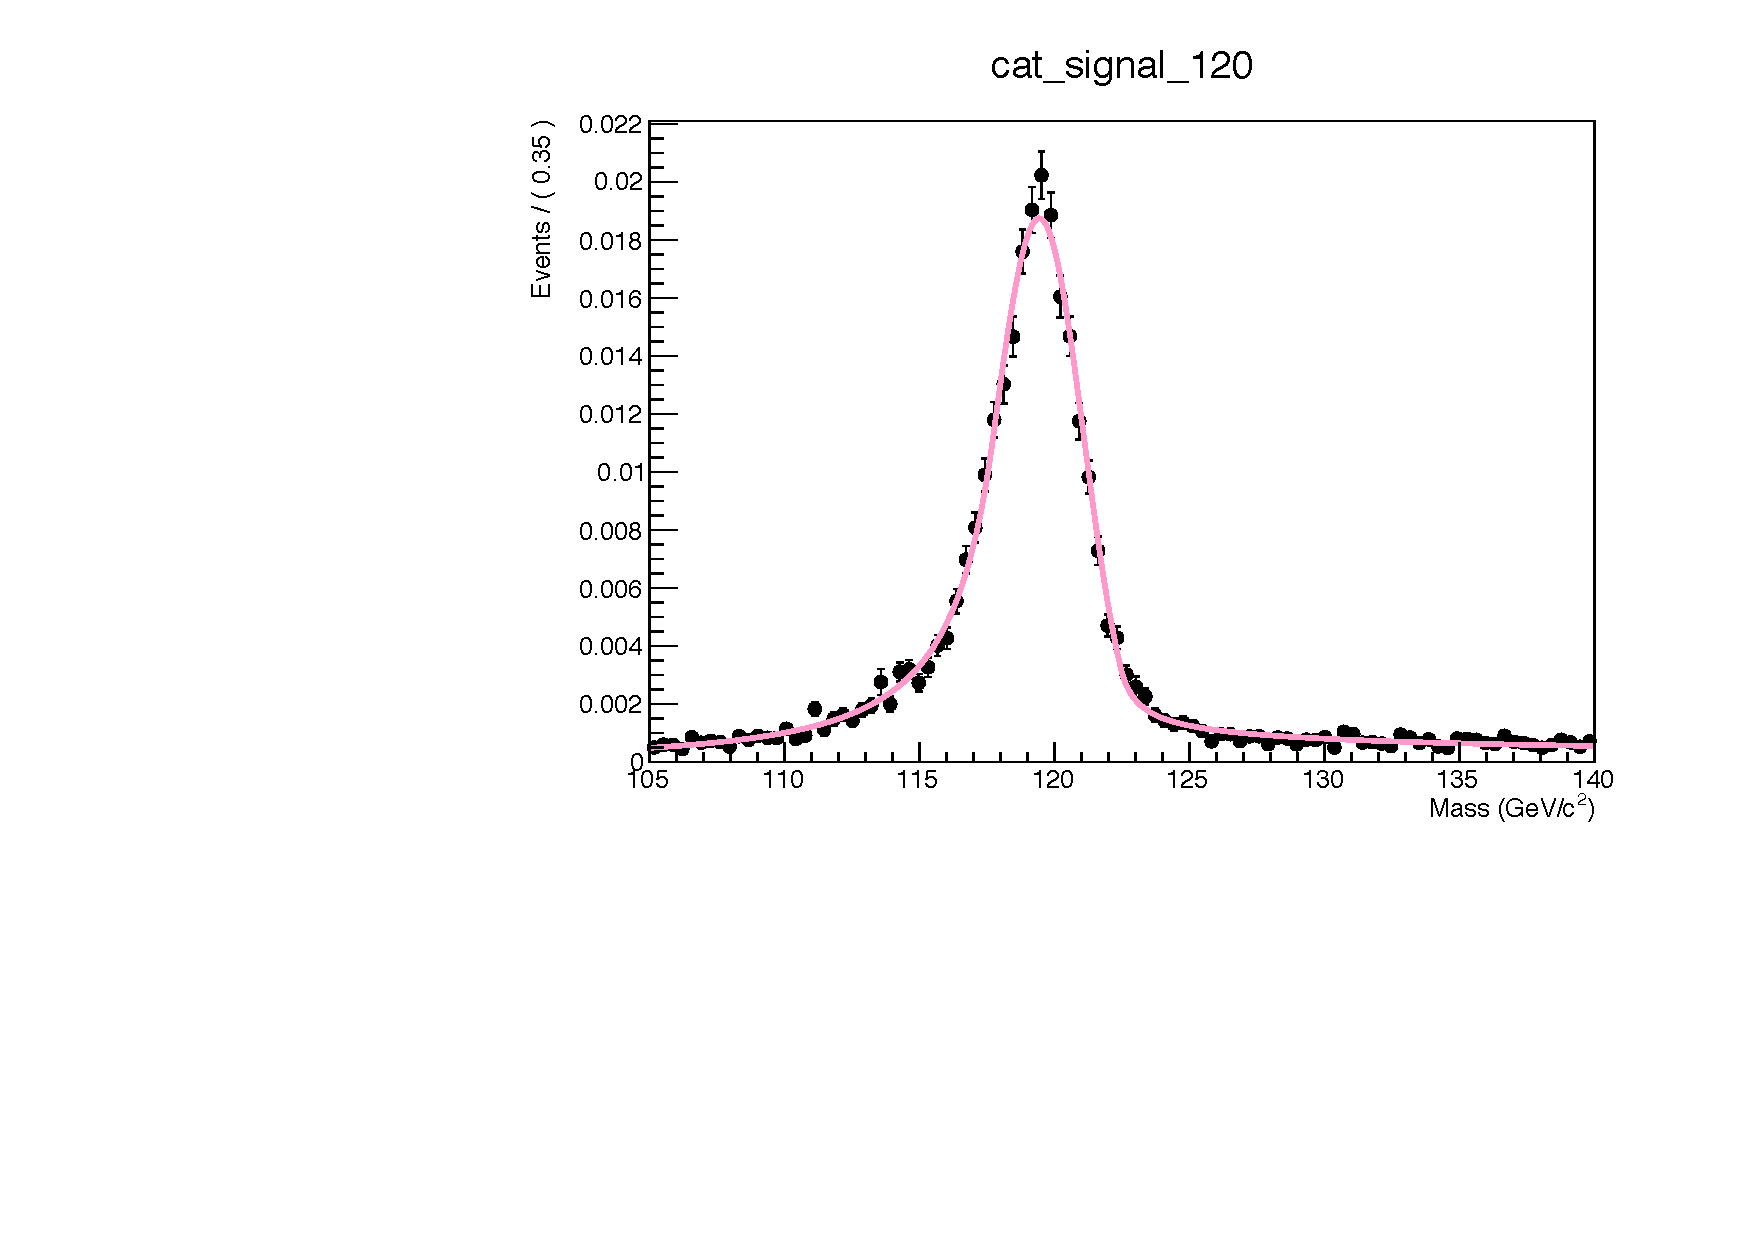
\includegraphics[width=0.3\textwidth]{Figures/SignalModelling/Signal_Parametrization/2018/ttH_2e2mu_2018_120_Sim.pdf}
%		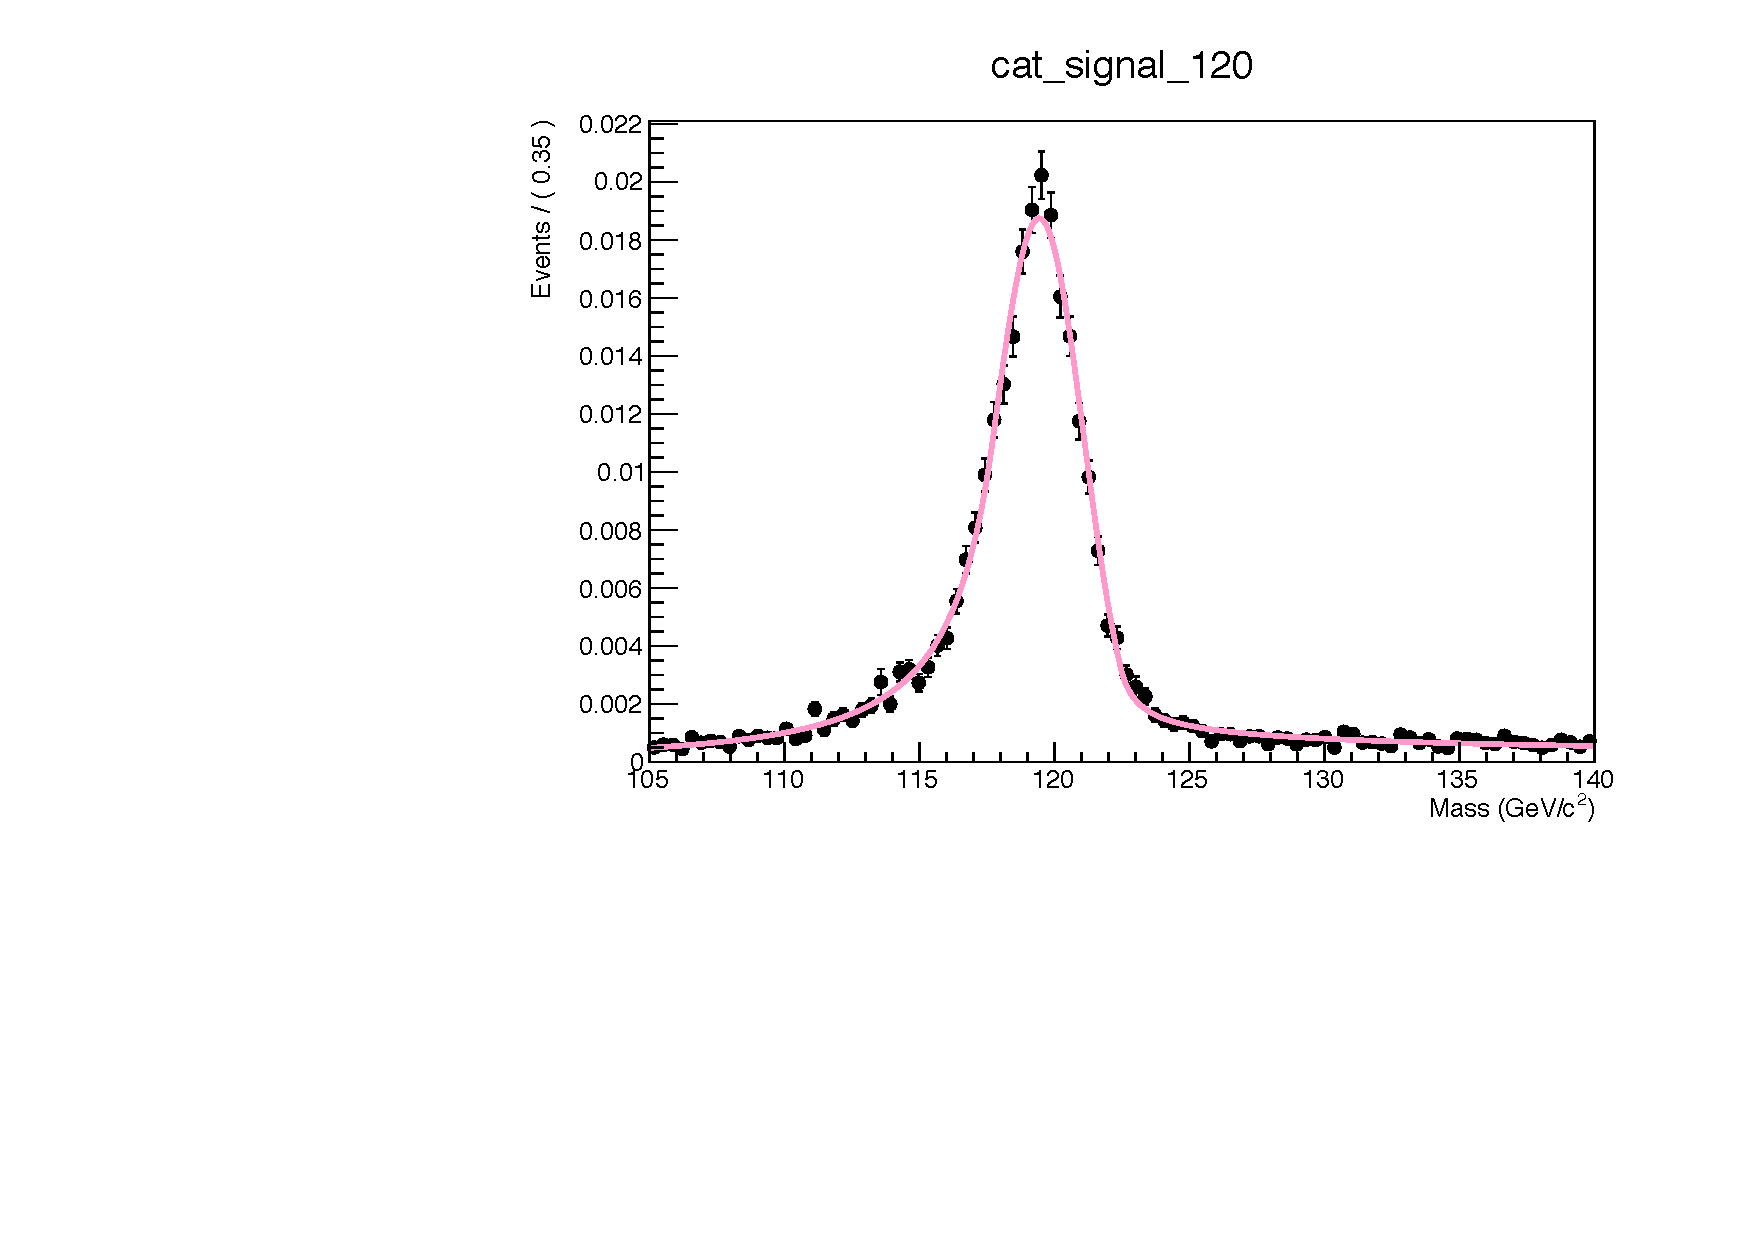
\includegraphics[width=0.3\textwidth]{Figures/SignalModelling/Signal_Parametrization/2018/ttH_2e2mu_2018_120_Sim.pdf}
%   		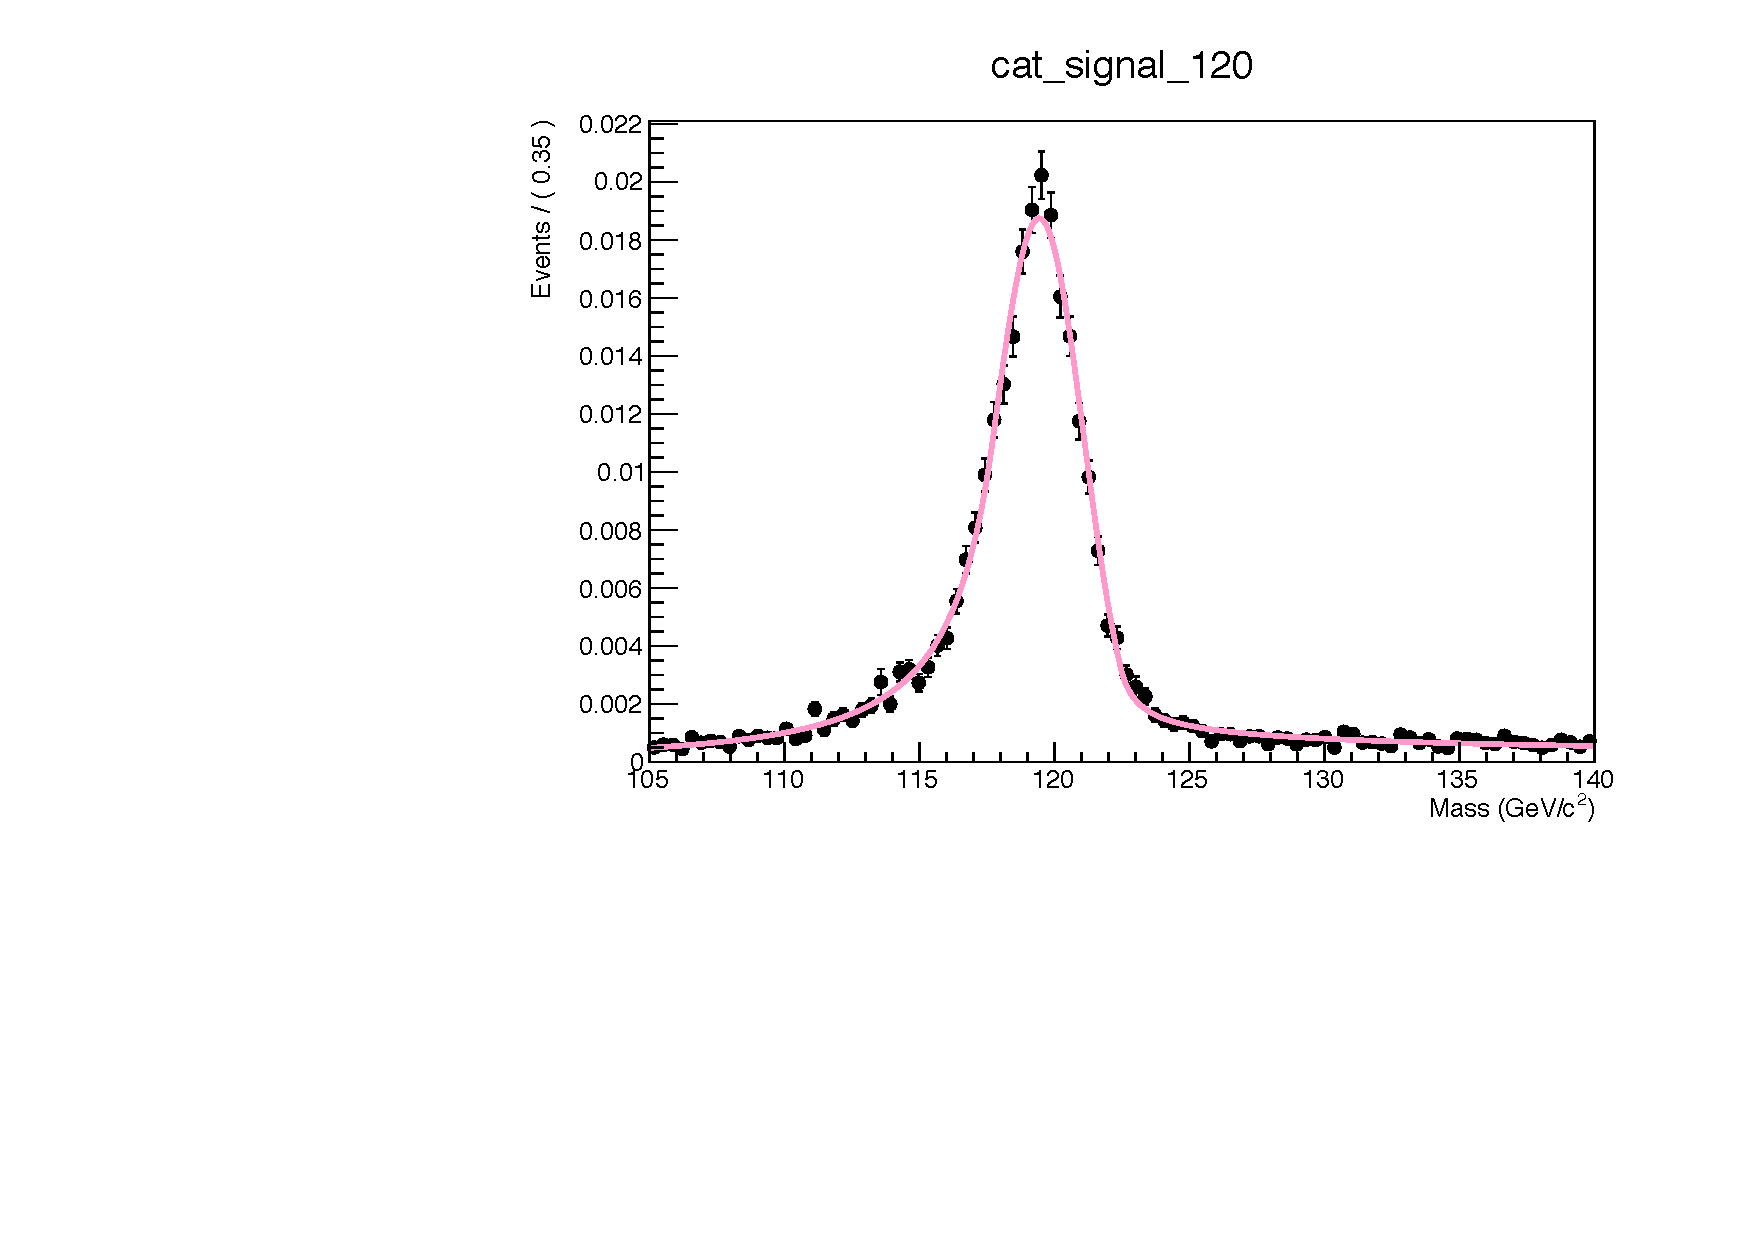
\includegraphics[width=0.3\textwidth]{Figures/SignalModelling/Signal_Parametrization/2018/ttH_2e2mu_2018_120_Sim.pdf}
%		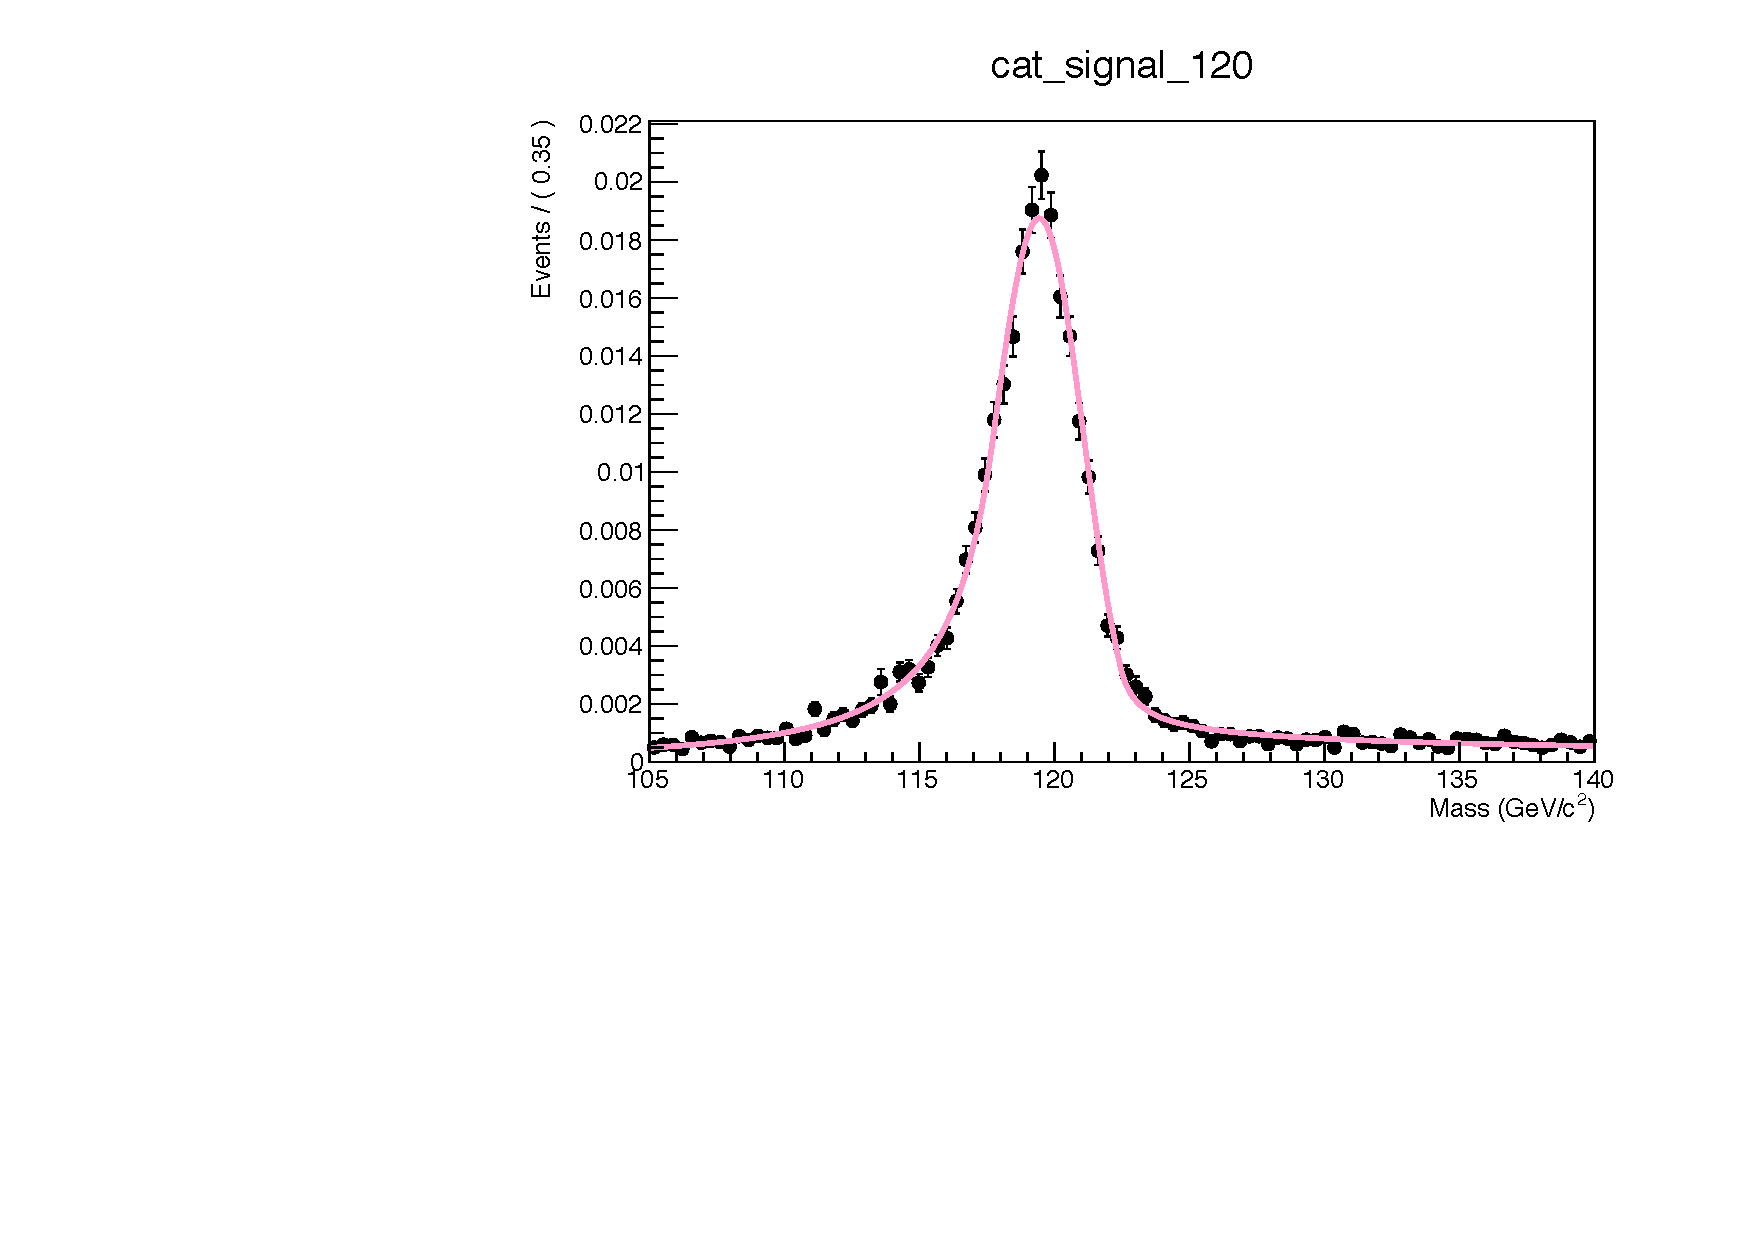
\includegraphics[width=0.3\textwidth]{Figures/SignalModelling/Signal_Parametrization/2018/ttH_2e2mu_2018_120_Sim.pdf} 
%		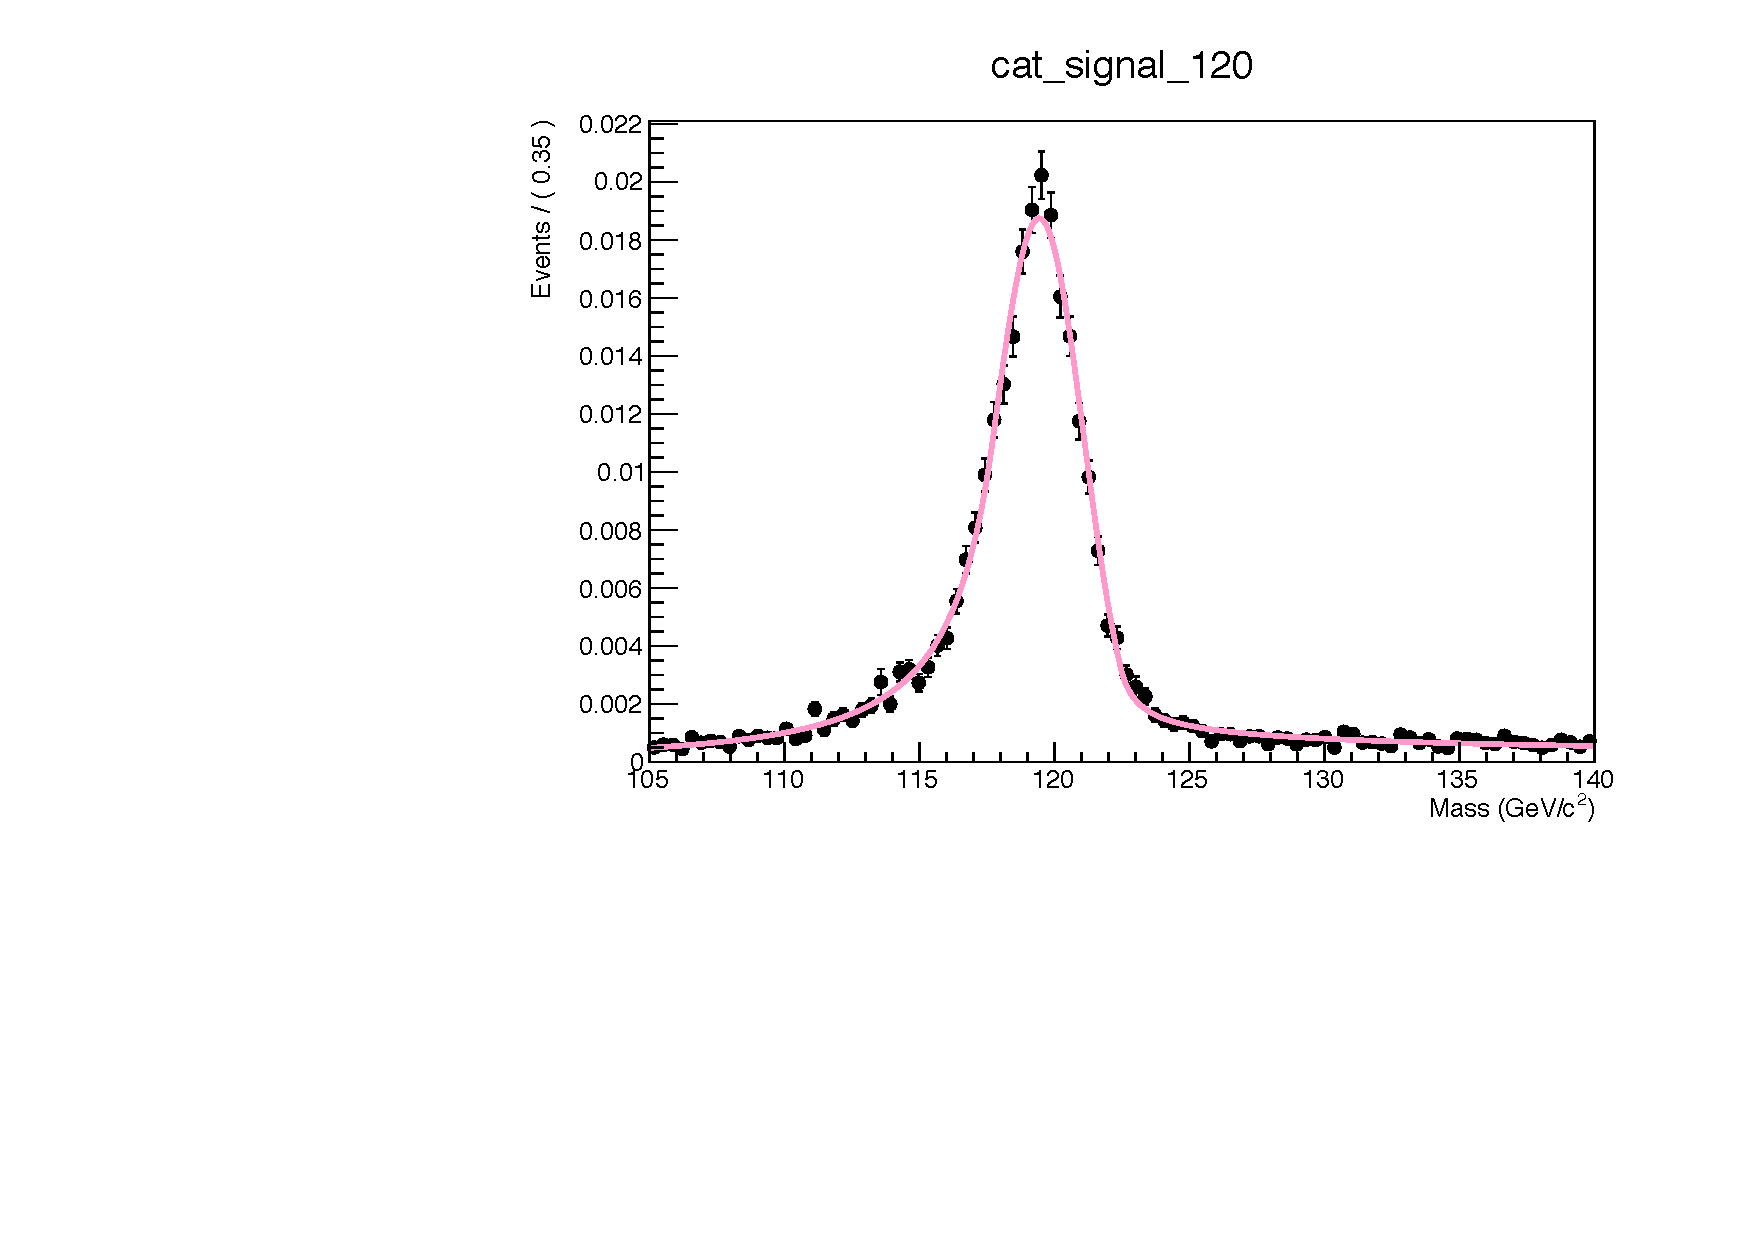
\includegraphics[width=0.3\textwidth]{Figures/SignalModelling/Signal_Parametrization/2018/ttH_2e2mu_2018_120_Sim.pdf}
%		\caption{Simultaneous fit for ggH production mode, in 2018, for different mass points, 
%		in 2e2$\mu$ final state.}
%	\label{signal_lineshape_2018_full_2}
%	\end{center}
%\end{figure}
% TODO:REWORD
 \subsection{Building the 1D pdf}
 Higgs boson mass measurement is firstly extracted from a one-dimentional likelihood function 
 $\mathcal{L}$($m_{4\ell}|m_{H}$), where $m_{H}$ is fixed to the value of 125 GeV. 
 The model and the normalisation used for the signal are described in \ref{sec:SignalNormalization}.\\
 As referece, Fig.~\ref{fig:1D_mass_2018_ggH} shows the four-lepton invariant mass distribution in 
 the signal region ([105-140]\GeV) using ggF events, with the DSCB fit for 2018, split in four 
 different final states.
 \begin{multiFigure}
    \centering
    \addFigure{0.48}{figures/higgsmassmeas/ggH_MassDistribution/1D_mass_2018_ggH_4mu.pdf}
    \addFigure{0.48}{figures/higgsmassmeas/ggH_MassDistribution/1D_mass_2018_ggH_4e.pdf}
    \addFigure{0.48}{figures/higgsmassmeas/ggH_MassDistribution/1D_mass_2018_ggH_2e2mu.pdf}
    \addFigure{0.48}{figures/higgsmassmeas/ggH_MassDistribution/1D_mass_2018_ggH_2mu2e.pdf}
    \captionof{figure}
        [TODO]
        {Four-lepton invariant mass distribution in the signal region ([105--140]\GeV) using ggH events, with the DSCB fit for 2018: 4\Pmu (top left), 4e (top right), 2e2\Pmu (bottom left), $2\Pmu2\Pe$ (bottom right).}
    \label{fig:1D_mass_2018_ggH}
\end{multiFigure}

%The 1D likelihood scans vs \mH, while profiling signal strength $\mu$ as all other nuisance parameters, are 
%shown in \figurename~\ref{1D_model}. 
%%All systematic errors are included. In order to estimate the 
%%contribution of the statistical and systematic error to the mass measurement, a likelihood scan removing 
%%both the normalization and shape systematics is performed. As in the case of the scan including the full 
%%uncertainties, $\mu$ is profiled, and then its uncertainty is included in the statistical error, because 
%%its magnitude represents the amount of signal events fitted, and then it has statistical nature. 
%%The systematic uncertainty is estimated as the difference in quadrature between the full uncertainty 
%%and the statistical uncertainty. 
%Results are summarised in ~\tablename~\ref{table:1D_model_result}.
%\begin{figure}[!htbp]
%	\begin{center}
%		\includegraphics[width=0.35\textwidth]{Figures/Placeholder.png}
%		\includegraphics[width=0.35\textwidth]{Figures/Placeholder.png}
%		\caption{1D likelihood scan as a function of mass for 1D fit scenario for the combination of 
%		all final states (left). Solid lines represents the scan with full uncertainties included, 
%		dashed lines statistical error only.  Results for each final state is shown on the right.}
%		\label{1D_model}
%	\end{center}
%\end{figure}
%



%%%%%%% 
%%%%%%% 
% plots about normalisation will be shown only for 1D_VXBS_Z1 configuration
%%%%%%% 
%%%%%%% 
%Examples of the fit procedures are shown in \figurename~\ref{signal_lineshape_2016_width}, 
%\ref{signal_lineshape_2017_width},  \ref{signal_lineshape_2018_width}.
%\begin{figure}[!htbp]
%	\begin{center}
%   		\includegraphics[width=0.3\textwidth]{Figures/HiggsWidth/2016_4Mu.png}
%		\includegraphics[width=0.3\textwidth]{Figures/HiggsWidth/2016_4Ele.png}
%		\includegraphics[width=0.3\textwidth]{Figures/HiggsWidth/2016_2Ele2Mu.png}
%		\caption{Signal lineshape for 2016: 4$\mu$ on left, 4e in the middle, 2e2$\mu$ on right.}
%	\label{signal_lineshape_2016_width}
%	\end{center}
%\end{figure}
%\begin{figure}[!htbp]
%	\begin{center}
%   		\includegraphics[width=0.3\textwidth]{Figures/HiggsWidth/2017_4Mu.png}
%		\includegraphics[width=0.3\textwidth]{Figures/HiggsWidth/2017_4Ele.png}
%		\includegraphics[width=0.3\textwidth]{Figures/HiggsWidth/2017_2Ele2Mu.png}
%		\caption{Signal lineshape for 2017: 4$\mu$ on left, 4e in the middle, 2e2$\mu$ on right.}
%	\label{signal_lineshape_2017_width}
%	\end{center}
%\end{figure}
%\begin{figure}[!htbp]
%	\begin{center}
%   		\includegraphics[width=0.3\textwidth]{Figures/HiggsWidth/2018_4Mu.png}
%		\includegraphics[width=0.3\textwidth]{Figures/HiggsWidth/2018_4Ele.png}
%		\includegraphics[width=0.3\textwidth]{Figures/HiggsWidth/2018_2Ele2Mu.png}
%		\caption{Signal lineshape for 2018: 4$\mu$ on left, 4e in the middle, 2e2$\mu$ on right.}
%	\label{signal_lineshape_2018_width}
%	\end{center}
%\end{figure}
    